\documentclass[12pt,phd,a4paper,oneside]{thesis}

% -------- Packages --------

\usepackage{blindtext}
\usepackage{emptypage}

\usepackage[rgb,dvipsnames]{xcolor}
\usepackage[format=hang,font=small,labelfont=bf,hypcap=false]{caption,subcaption}
\usepackage{graphicx,tikz,listings,color,float}
\renewcommand\thesubfigure{\Alph{subfigure}}

\usetikzlibrary{shapes.geometric,arrows}
\restylefloat{figure}
\graphicspath{{figures/}}

\usepackage{amsmath,amssymb,amsfonts,bbold}
\usepackage{booktabs} % pretty tables
\usepackage[version=4]{mhchem}

\usepackage{gensymb}
\usepackage{textcomp}

\usepackage{setspace}
\setstretch{1.5}

\usepackage{multirow}
\usepackage{bibentry} 
\usepackage{etoolbox}

\usepackage[normalem]{ulem}
\usepackage[T1]{fontenc}
\usepackage[utf8]{inputenc}

\let\altmathbb\mathbb
\usepackage[sc]{mathpazo}
\AtBeginDocument{\let\mathbb\altmathbb}

\usepackage{epigraph} %quotes
\usepackage{musixtex}

\setlength\epigraphwidth{.8\textwidth}

\usepackage{notoccite}% PREVENTS CITES IN CAPTIONS FROM MISNUMBERING YOUR REFERENCES 
\usepackage{pdfpages}
%   General parameters, for ALL pages:
\renewcommand{\topfraction}{0.9}	% max fraction of floats at top
\renewcommand{\bottomfraction}{0.8}	% max fraction of floats at bottom

%   Parameters for TEXT pages (not float pages):
\setcounter{topnumber}{2}
\setcounter{bottomnumber}{2}
\setcounter{totalnumber}{4}     % 2 may work better
\setcounter{dbltopnumber}{2}    % for 2-column pages
\renewcommand{\dbltopfraction}{0.9}	% fit big float above 2-col. text
\renewcommand{\textfraction}{0.07}	% allow minimal text w. figs

%   Parameters for FLOAT pages (not text pages):
\renewcommand{\floatpagefraction}{0.7}	% require fuller float pages
\renewcommand{\dblfloatpagefraction}{0.7}	% require fuller float pages

\AtBeginDocument{\DeclareGraphicsExtensions{.pdf,.PDF,.eps,.EPS,.png,.PNG,.tif,.TIF,.jpg,.JPG,.jpeg,.JPEG}}

\newenvironment{Figure}
{ \begin{figure}[H] \centering{} \setlength\unitlength{1cm}  \captionsetup{format=plain}  }
{ \end{figure} } % For things like figures and tables
% defining commands for creating flowcharts
\tikzstyle{startstop} = [rectangle,rounded corners,minimum width=3cm,minimum height=1cm,text centered,draw=black,fill=gray!30]
\tikzstyle{io} = [trapezium, trapezium left angle=70, trapezium right angle=110, minimum width=3cm, minimum height=1cm, text centered, draw=black]
\tikzstyle{process} = [rectangle, minimum width=3cm, minimum height=1cm, text centered, draw=black, fill=gray!30]
\tikzstyle{decision} = [diamond, minimum width=3cm, minimum height=1cm, text centered, draw=black, fill=yellow!30]
\tikzstyle{arrow} = [thick,->,>=stealth]

% defining python syntax highlighting environment
\DeclareFixedFont{\ttb}{T1}{txtt}{bx}{n}{9} % for bold
\DeclareFixedFont{\ttm}{T1}{txtt}{m}{n}{9}  % for normal

% python syntax colors
\definecolor{deepblue}{rgb}{0,0,0.5}
\definecolor{deepred}{rgb}{0.6,0,0}
\definecolor{deepgreen}{rgb}{0,0.5,0}

% Python style for highlighting
\newcommand\pythonstyle{\lstset{
language=Python,
basicstyle=\ttm,
otherkeywords={self},             % Add keywords here
keywordstyle=\ttb\color{deepblue},
emph={MyClass,__init__},          % Custom highlighting
emphstyle=\ttb\color{deepred},    % Custom highlighting style
stringstyle=\color{deepgreen},
frame=tb,                         % Any extra options here
showstringspaces=false            %
}}

% python environment and inline
\lstnewenvironment{python}[1][]{
  \pythonstyle
  \lstset{#1}
}{}
\newcommand\pythoninline[1]{{\pythonstyle\lstinline!#1!}}

% mathematical formatting
\newcommand{\Vector}[1]{\vec{#1}}
\newcommand{\Matrix}[1]{\mathbf{#1}}

\newcommand{\dt}{\mathrm{d}t}

\newcommand{\edit}{\textcolor{blue}}
\newcommand{\stolen}{\textcolor{red}}
\newcommand{\duplicate}{\textcolor{teal}} %duplicate w/ methods in paper(s) -- may need further depth in intro

\newcommand{\rates}{F_{\theta}}
\newcommand{\tangent}{T_{\theta}}
\newcommand{\steadystates}{\partial S_{\theta}}

\newcommand{\Det}{\left| \frac{\partial\rates}{\partial u} \right|}
\newcommand{\measure}{\varphi_{\theta}}

\newcommand{\predictions}{\mathcal{P}}
\newcommand{\targets}{\mathcal{D}}
\newcommand{\loss}{L}
\newcommand{\error}{E}
\newcommand{\Reals}{\mathbb{R}}
\newcommand{\steady}{u^*}
\newcommand{\cycle}{\omega}
\newcommand{\jacobian}{\frac{\partial\rates}{\partial u}}
\newcommand{\eigenvector}{\hat{v}_\lambda}
\newcommand{\e}{\mathbb{e}}
\newcommand{\degenerate}{u^{-}}
\newcommand{\critical}{u^\star}
\newcommand{\Real}{\Re\mathrm{e}}
\newcommand{\Imag}{\Im\mathrm{m}}
\newcommand{\where}{\quad\mathrm{where}\quad}

\makeatletter
\AtBeginDocument{
    \hypersetup{
        pdfsubject={Biophysics},
        pdfkeywords={inference,bifurcations},
        pdfauthor={Grisha Szep},
        pdftitle={Inferring bifurcations between phenotypes},
    }
}
\makeatother

\bibliographystyle{unsrt}  % For bibliographies
\setcounter{secnumdepth}{3}
\setcounter{tocdepth}{3}
\setboolean{@twoside}{false}

\begin{document}
\raggedbottom % stops huge gaps between paragraphs

\title{Inferring bifurcations\\between phenotypes}
\author{Grisha Szep}

\department{Randall Division of Cell \& Molecular Biophysics}
\sponsor{Microsoft Research Cambridge}

\date{October 29, 2021}
\maketitle
% \makedeclaration

\begin{abstract} % 300 word limit

    The gene-expression history of an organism and its environment determine the organism's phenotype. The phenotype is an inherently qualitative state, deduced by relative biochemical concentration measurements collected by methods such as flow cytometry or fluorescence microscopy. The biochemical threshold concentrations that distinguish different phenotypes can be modelled by applying bifurcation analysis to differential equation models and the search for these boundaries in experimental data can be done using dimensionality reduction and clustering techniques. This establishes a relationship between bifurcations, phenotypes and machine learning techniques that are the subject of this thesis.

    % The first chapter presents an interactive tool for exploring phenotypes in flow cytometry data. In particular we explore a multi-tissue, high-dimensional, immune cell dataset. The tool bridges machine learning methods and the popular FlowJo, used to annotate cells with gating strategies. An assortment of dimensionality reduction techniques are applied to create two dimensional embeddings and confusion matrices are used to quantify annotation agreement between immunologists. By leveraging the geospatial mapping library OpenLayers to render, annotate and analyze cells, immunologists can now efficiently navigate the phenotype space of Human Cell Atlas datasets.
    
    % The next chapter focuses on a model-driven approach for exploring and designing phenotypes, where we demonstrate how model-guided design of synthetic E. Coli can elucidate pattern formation mechanisms in multicellular development. We infer the parameters of a biochemically motivated system of differential equations against time course fluorescence data acquired from plate reader experiments. Our design goals however were not in the temporal domain, rather we wanted to control the shape and size of a cusp bifurcation in the space of experimentally controlled input concentrations.
    
    % To address these limitations, I define a differentiable semi-supervised cost function that uses bifurcation locations as targets. Bifurcations are encouraged by an unsupervised term that extremises the curvature of the determinant of the Jacobian. By exploring the cost landscape for minimal models that span the space of saddle-nodes and pitchforks, I show that the parameter space basins define regions of qualitatively equivalent differential equations. The differentiability of the cost function enables efficient optimisation using libraries such as Flux.jl that leverage automatic differentiation. The impact of this work would enable experimentalists to efficiently navigate design spaces of differential equation models.
    
\end{abstract}
\newpage
\clearpage
\begin{center}
    \thispagestyle{empty}
    \vspace*{\fill}
    \epigraph{
        Blank pages are the worst.\\
        They impose a glaring responsibility onto someone to fill it with meaningful content.\\
        Much like other starting points:
        a new job, a marble stone, empty land, all future that tower over you, forcing the person facing it to ask:\\
        "do I really want to do this?"\\
        Blank pages are the worst.\\
        They reflect a glaring light upon you, reflecting the messages that would otherwise happinly bounce around in the ether, along with memories, desires, unfinished projects, and other concofonous bullshit in your head.\\
        A whole page!\\
        Rejoice at the etchings of achievement. You've started now so don't give up, or stop, you'll look stupid. Now make sure you go back and edit the previous page so that other will not know how stupid you are.\\
        Edit it, edit it,\\
        edit it into oblivion untill you can't recognise whether you are editing the page or yourself.}{}
    \vspace*{\fill}
\end{center}
\clearpage

\begin{acknowledgements}
    The past four years of my life have been full of excitement, creativity and exploration, none of which would have been possible without the support of Attila and Neil. Their mentorship and guidance has been a shining example of leadership and whose qualities I will take with me into future roles. I would like to thank my colleagues and friends at Microsoft Research, whose diverse projects in biotechnology captured my imagination.

    I would like to acknowledge Valerie Coppard, who was an absolute pleasure to work with and introduced me to Joanne Jones' lab at Cambridge University, catalysing the \emph{FlowAtlas.jl} project. Her enthusiasm...

    I would like to thank Matilda Peruzzo and Silvia Cabaliero During the pandemic. I would like to thank Mohammed Ali

    I am thankful to my friends at Burnt Umber who run a cozy and welcoming cafe in Hackney Wick, where I wrote a large chunk of my thesis, felt supported and cared for during difficult times. Disree Shaw my therapist. Fraser...

    I would like to thank family and dad
\end{acknowledgements}

%%%%%%%%%%%%%%%%%%%%%%%%%%%%%%%%%%%%%%%%
%%%%%%%%%%%%%%%%%%%%%%%%%%%%%%%%%%%%%%%%
%%%%%%%%%%%%%%%%%%%%%%%%%%%%%%%%%%%%%%%%
%%%%%%%%%%%%%%%%%%%%%%%%%%%%%%%%%%%%%%%%
%%%%%%%%%%%%%%%%%%%%%%%%%%%%%%%%%%%%%%%%

\setcounter{tocdepth}{2} 
% Setting this higher means you get contents entries for
%  more minor section headers.

\tableofcontents
\listoffigures
\chapter{Introduction \& Motivation}
\label{chapter:introduction}
\begin{music}
    \parindent10mm \instrumentnumber{1} \setstaffs1{1} 
    \generalmeter{\meterfrac34} \generalsignature{3}
    \startextract
            \Notes \Dqbu dk \zhl{i*} \en
        \bar
            \Notes \Dqbu hi \zhu{h*} \en
    \zendextract
\end{music}
\epigraph{\textit{one thing that won't change with time is the memories of younger years}}{Minuet of Forest --- Ocarina of Time}

We are living in the wake of milestones in biotechnology and computational biology that suggest reverse-engineering cell biology is within our grasp. The coronavirus pandemic accelerated investment in biotechnology \cite{DeFrancesco2021Financing2020}. The fields of synthetic and systems biology are beginning to resemble engineering disciplines; genetic engineering is becoming more precise, high-throughput single-cell experiments are performed by robots and measurements across all levels of the central dogma are possible: genomics, transcriptomics, proteomics and metabolomics \cite{Perkel2021Single-cellAge}. Advances in micro-fabrication \cite{Shafiee2017TissueMedicine} and in-vitro reconstitutive methods \cite{Gopfrich2018MasteringCells} have allowed biologists to isolate pathways and mechanisms to a level of mathematical and computational tractability \cite{Sharpe2017ComputerTomorrow.}.

The complexity barrier in biology poses a significant challenge. Multiple levels of organisation from the molecular, to cellular, to the whole organism interact with each other, which makes scale separation and accurate approximations difficult. Furthermore, the combinatorial space of possible interactions between macro-molecules involved in the central dogma is intractably large. Systems and synthetic biology have historically made progress through a process of brute force trial and error. This usually involves the interaction of many custom-made parts that are iteratively optimised by human intervention. A trend first observed in the 1980s known as \textit{Eroom's law} revealed that discoveries in biotechnology are becoming slower and more expensive over time, despite improvements in technology \cite{Scannell2012DiagnosingEfficiency}. This problem is exemplified by the declining success rate of clinical trials in the drug discovery process \cite{Wong2019EstimationParameters} and compounded by the ongoing reproducibility crisis \cite{Ioannidis2005WhyFalse.,Mullard2021HalfEffort}. It appears that much of the low-hanging fruit has been picked \cite{Earm2014IntegrativeDevelopment} with methodologies whose standards for transparency, reproducibility and accessibility leave us with much to be desired. 

Despite the widespread lack of mechanistic understanding in human cell biology, sophisticated engineering goals such as targeted modification of the immune system are now possible. In 2018, a T-cell gene therapy --- \emph{tisagenlecleucel} \cite{Halford2021TisagenlecleucelConsiderations} --- for the treatment of adolescent and young adult acute lymphoblastic leukaemia became the most expensive cancer therapy ever, at \$475,000 \cite{Hernandez2018TotalImmunotherapy}. Here, the high cost results from a hugely complex procedure for administering the treatment, which involves harvesting patient T-cells and engineering them to express a novel chimeric antigen receptor (CAR), and then returning the modified T-cells back into the patient. Even in settings where biomanufacturing relies on specific known mechanisms, the manufacturing of viral vectors that deliver the gene therapy is far from straightforward. Human-derived producer cells are used to  synthesise vector \cite{Merten2016ProductionVectors}, but how to engineer them to carry this out efficiently depends on understanding the complexity of these complex cell-types, which involve a great number of unknown mechanisms. To provide clues into the biological processes that limit efficient bioproduction, omics data can be collected along key protocol stages in attempts to understand and optimise production.

After a decade of engineering advances in data science and machine learning, epitomised by deep learning methods, theoretical foundations on high-dimensional learning tasks are beginning to condense \cite{Bronstein2021GeometricGauges}. Many tasks such as computer vision \cite{mnist2012,imagenet2009}, playing Go \cite{Silver2016}, or protein folding \cite{Jumper2021HighlyAlphaFold} are in fact feasible with appropriate computational scale. Remarkably, the essence of deep learning is built from two simple algorithmic principles: the notion of lower-dimensional \emph{representation}, whereby group equivariant and invariant transformations are composed to capture the appropriate notion of regularity for each task \cite{Bronstein2021GeometricGauges}, and second, learning by local gradient-descent type methods enabled by \emph{differentiable programming} \cite{Innes2019AComputing}.

The emerging picture suggests that bringing together the advances in software and wetware in iterative hypothesis generation and discovery pipelines are key to overcoming the complexity barrier in biology \cite{Sharpe2017ComputerTomorrow.,Ringel2020BreakingLaw,AlQuraishi2021DifferentiableMechanisms}. The term \textit{in silico} has become popularised amongst biologists, which conceptualises a computational model, alongside \emph{in vitro} and \emph{in vivo}, as a method for investigating an organism \emph{in situ}. Researchers are going as far as conceptualising the \emph{digital twin} for personalised medicine \cite{Bjornsson2019DigitalMedicine}. Bringing together deep learning and biomedical research has the potential of importing the notions of \emph{representation} and \emph{differentiability} into biological engineering \cite{AlQuraishi2021DifferentiableMechanisms} and thereby reaping their benefits. Differentiability within engineering pipelines has the same advantage over brute force trial and error as it does over sampling-based algorithms and thereby decrease the time and cost for biological research. While not all equipment, data and resources used to perform a study can be shared, representations of a study in the form of computational models can increase transparency and reproducibility. Efforts towards open standards have gained traction over the past decade \cite{Malik-Sheriff2020BioModels15Science} with model sharing standards such as Systems Biology Markup Language \cite{Hucka2018TheCore} and data repositories like Human Cell Atlas
\cite{Regev2017TheAtlas} and Flow Repository \cite{Spidlen2012PreparingFlowRepository.org}. The open standards and ethical thresholds of deep learning are also increasing, with the formation of OpenAI \cite{Brockman2016OpenAIGym} and sharing standards such as ONNX \cite{Bai2019ONNX:Exchange}.

\section{Representation of Single Cells}

In this thesis, the focus is on differential equation representations of single cells. In this section we give a brief motivation behind why differential equations are convenient, what other representations exist and how results may translate between differential equations and other representations. When studying a particular biological phenomenon, the appropriate spatio-temporal scale must be chosen that simplifies the mechanism under study while preserving the relationships between experimentally accessible parameters and the resultant behaviours. We do not expect a single unifying tractable model of biological mechanisms under study. In practice there exist multiple equally valid models with various degrees of complexity. For example, the immune system can be described with agent-based models \cite{} and also with ordinary differential equations \cite{}. The set of equations can describe all molecular interactions within a cell \cite{}, or only the pathways under study \cite{}. In cases where tissue organisation or sub-cellular spatial mechanics are important, partial differential equations \cite{}, vertex models \cite{} and \cite{} can be used to characterise them.
\begin{Figure}
    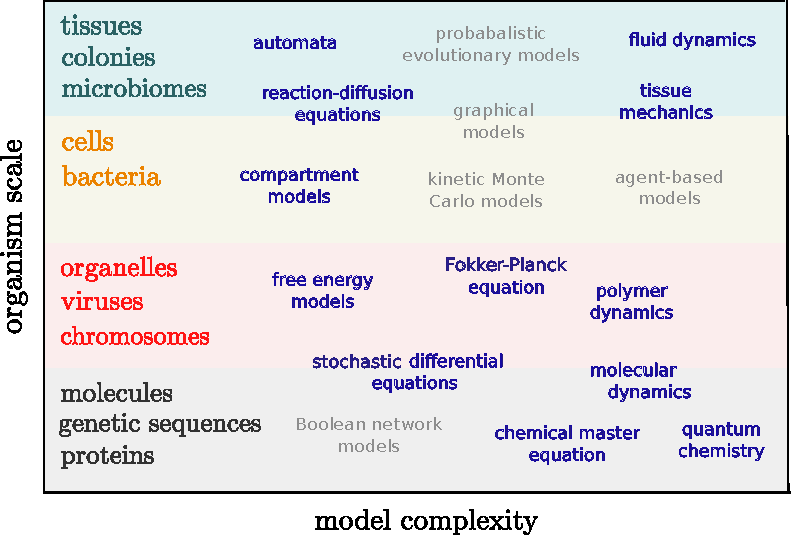
\includegraphics[width=0.9\linewidth]{figures/top-down-bottom-up}
    \caption{Biological models at different spatial scales and complexities, a large class of which can be cast into differential equation form indicated in bold blue}
    \label{fig:tdbu}
\end{Figure}
Differential equations are convenient because they are usually differentiable, continuous state and continuous time models and hence are already compatible with the two algorithmic principles of deep learning \cite{Bronstein2021GeometricGauges}. In the context of dynamical systems theory it is relatively simple to derive analogous results for discrete state or discrete time models: cellular automata \cite{Martin2017DifferentiableAutomata}, Markov chains \cite{Darling2008DifferentialChains}, stochastic processes and discrete maps just to name a few. A large class of biological models at different spatial scales can be cast into differential equation form (Figure \ref{fig:tdbu}), although this may not always be necessary. With the help of automatic differentiation, programs with arbitrary control flow become piecewise differentiable \cite{Gune2018AutomaticSurvey}. One of the main limitations to consider is the number of branches in the program due to conditional statements and whether there are non-zero derivatives either side of the conditional statement that provide meaningful information. Rule-based models such as agent-based models are examples of programs with many conditional branches often with no meaningful derivatives on either side of the condition. In such scenarios we must fall back to finite difference approaches, requiring a finite number of evaluations of the model. This can be done in a cost-effective way, only evaluating gradients that will likely benefit the optimisation.

Differential equations models span a large range of spatial and temporal scales. It is important to choose a time-scale and space-scale that is relevant to the problem. If one is interested in tissue dynamics, attempting to model DNA conformations within each cell will render the problem intractable. As George Box aptly put \textit{``most models are wrong but some are useful"} so the role of theoretical descriptions in these settings is not necessarily to describe the way reality \textit{is} but serve as tools to bridge the non-intuitive gap between bottom-up and top-down approaches \cite{Gopfrich2018MasteringCells,Powell2018HowScratch,Pezzulo2016Top-downLevel}.

\subsection{Model Selection \& Reduction}
With such a heterogeneous selection of models that are valid at different spatial and temporal scales it becomes increasingly important to develop tools to navigate the space of models. We want to organise and then choose between different models that explain the same phenomenon whilst also enumerating the set of phenomena that a single model can explain. This problem is known in machine learning as model selection \cite{Ding2018ModelOverview} and establishing relationships between models of varying complexity is know as model reduction \cite{Besselink2013AControl}. We will see in the following section that exploring the space of models inherently involves some form of iterative hypothesis generation workflow.

In the context of parameter inference \cite{Brunton2016SparseSINDYc,GorbachScalableSystems}, sloppiness and sensitivity analysis have been extensively used in the search for reduced models \cite{Daniels2008,Chis2016OnIdentifiability,Gutenkunst2007UniversallyModels,Gabor2017ParameterBiosystems,Villaverde2016StructuralModels}. Linear mappings between models that preserve stoichiometry and reactant structure were investigated \cite{Cardelli2014MorphismsFunction,Cardelli2017MaximalSystems} and computational tools based on partition-refinement were released \cite{Cardelli2017ERODE:Equations}. Structural similarity between reaction networks can be revealed by such mappings, elucidating the functional aspects of complex networks in terms of simpler networks. Nonlinear mappings between models that preserve high-level features without resorting to structural assumptions about the models were still lacking lacking and formed part of the motivation for developing the methods in Chapter \ref{chapter:inference}.

We will see how a suitably defined cost function that focuses on high-level features of a model enables navigation and organisation of models across various levels of complexity. Indeed the focus on higher-level features of differential equation models, such as geometry rather than kinetics, has already been gaining traction in 
pattern formation theory \cite{Halatek2018}.

\subsection{Phenotyping in Flow Cytometry}

\section{Differentiability in Biological Engineering}

\subsection{Differentiable Programming}

While there is a clear mathematical definition of what a \emph{differentiable program} \cite{Innes2019AComputing} is, what does it mean for engineering in biology to be differentiable? In the effort to move past brute force trial and error methods, a standard for the \emph{design--build--test--learn} cycle has emerged in synthetic biology (Figure \ref{fig:dbtl}). This workflow has now been established as a paradigm \cite{Carbonell2018AnChemicals,Opgenorth2019LessonsLearning} with some aspects that have been automated by liquid handling robots, bioreactor environments and image processing pipelines. However, humans in the loop and custom moving parts still persist. Defining the boundary between parts that can be automated, and parts that need regular intervention by domain experts is a challenge \cite{Abate2018ExperimentalSemantics}.
\begin{Figure}
    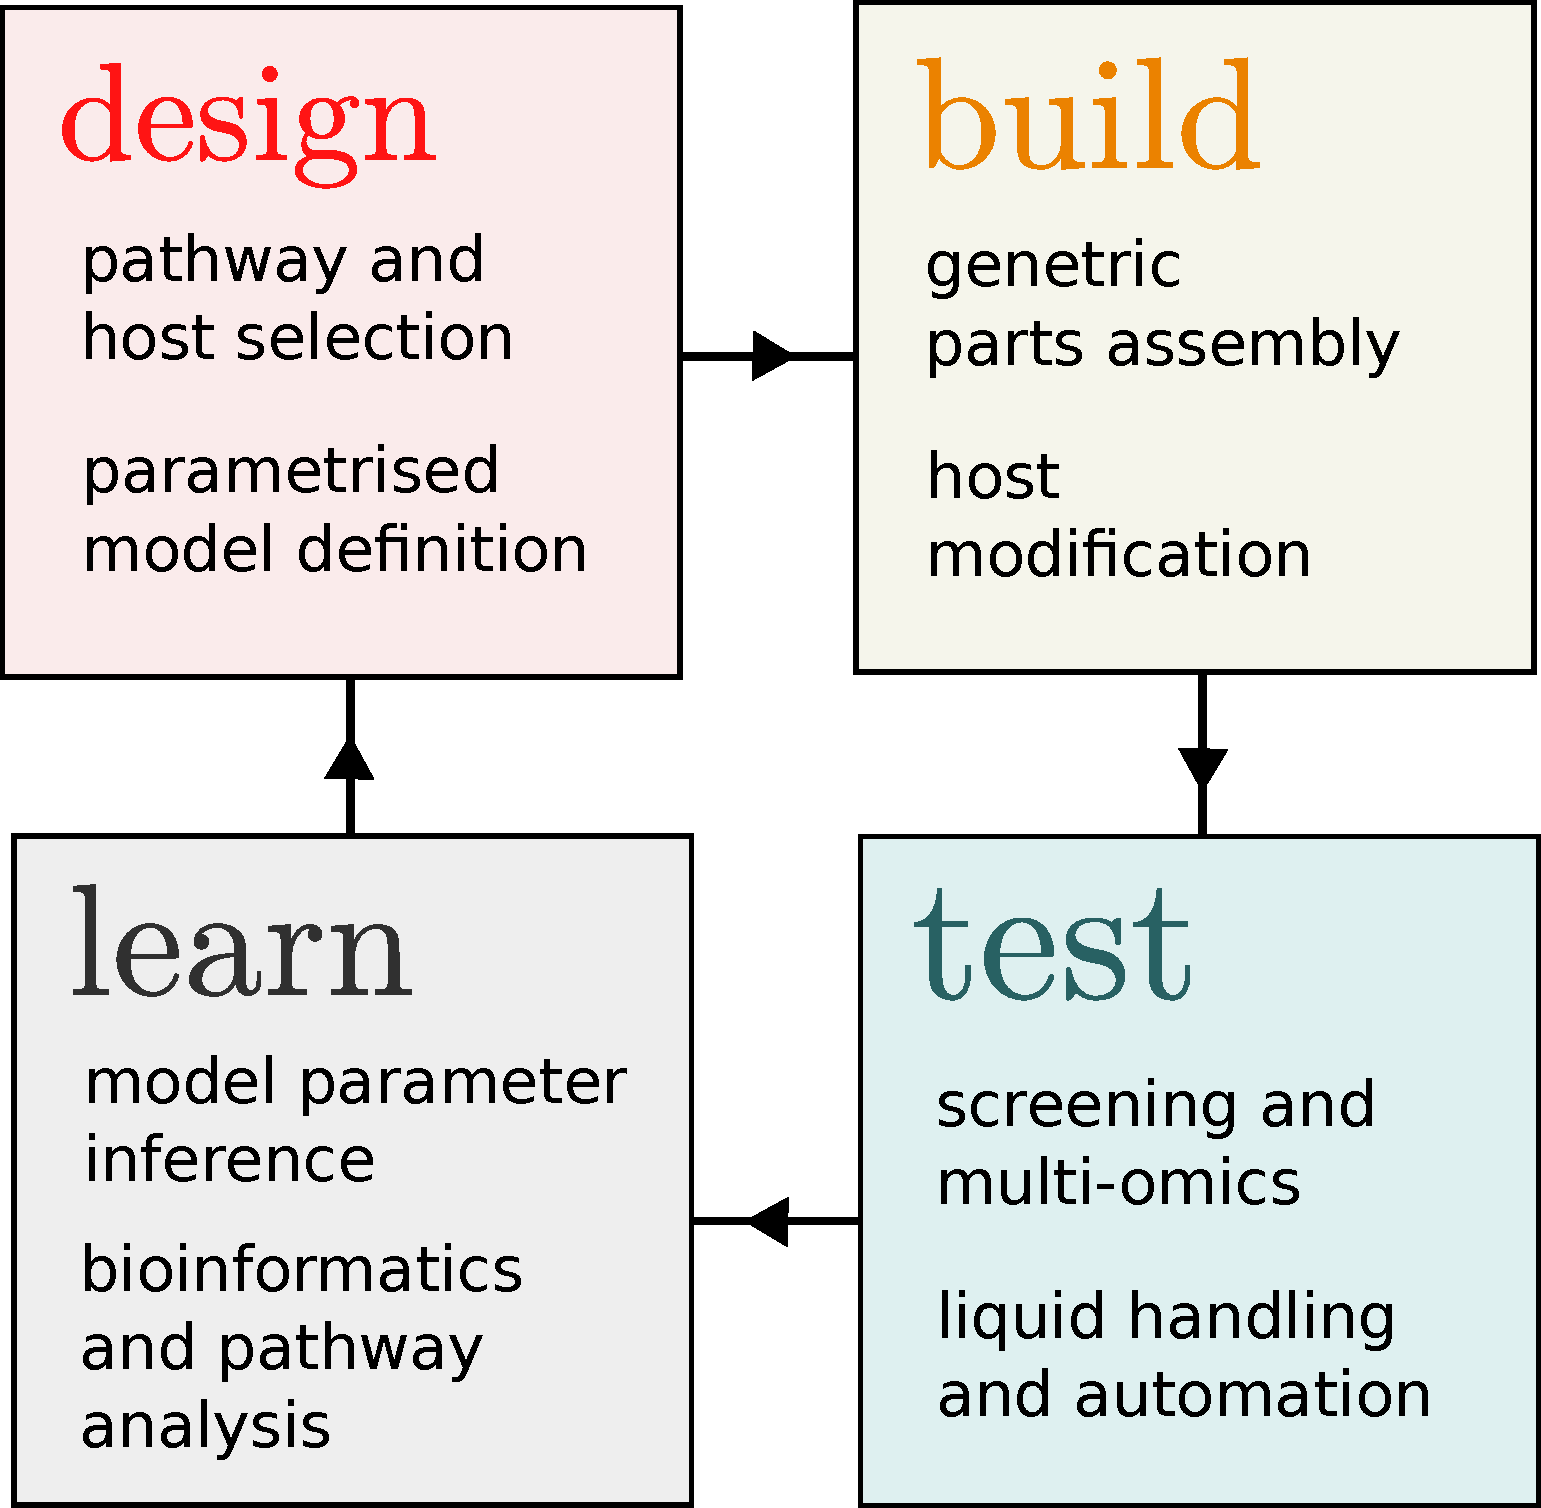
\includegraphics[width=0.6\linewidth]{figures/dbtl}
    \caption{\emph{design--build--test--learn} cycle from synthetic biology. This cycle is differentiable if a domain expert can track changes in any observation pair \emph{X,Y} along the pipeline}
    \label{fig:dbtl}
\end{Figure}
In principle such a pipeline is differentiable if a domain expert can efficiently get an answer questions like: \emph{What happens to Y when I change X?} or \emph{Which X do need to change in order to change Y?} for as many observable pairs \emph{X,Y} as possible. Furthermore, suitable experiments are identified to the capture the relevant data.

The \emph{design--build--test--learn} paradigm was used during the interdisciplinary collaboration described in Chapter \ref{chapter:double-exclusive}. In this thesis we focus on the \emph{design--learn} part of this workflow. One of the main learnings, as we shall see, from applying this paradigm is that, in order for the lab to converge onto their cell design goals efficiently, the workflow must be bidirectional, rather than a cycle. This way each part of the workflow can operate with its neighbours independently, without being blocked by other parts of the workflow.

\subsection{Design--Learn Workflow}
\label{section:design-learn}
Let us focus on the \emph{design--learn} part of the workflow in the context of model inference. Partial knowledge of mechanisms in biology has given rise to a class of models that have been coined as \emph{grey box models} \cite{Meeds2019EfficientSystems}. In this setting, domain expertise dictates which aspects of the model are highly structured with specific hypotheses and which are composed with generic transformations that obey a chosen set of group symmetries.
\begin{Figure}
    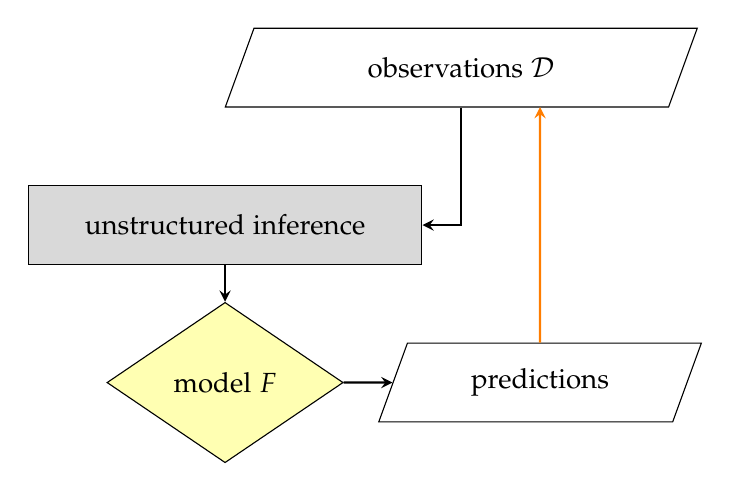
\begin{tikzpicture}[node distance=2cm]

        \node (nonparametric) [process, minimum width=5cm] {unstructured inference};
        \node (data) [io, right of=nonparametric, xshift=1cm, yshift=2cm] {observations $\mathcal{D}$};

        \node (field) [decision, below of=nonparametric] {model $F$};
        \node (pred) [io, right of=field,  xshift=2cm] {predictions};

        \draw [arrow] (data) |- (nonparametric);
        \draw [arrow] (nonparametric) -- (field);
        
        \draw [arrow] (field) -- (pred);
        \draw [arrow,color=BurntOrange] (pred) -- +(0,3.5);

    \end{tikzpicture}
    \caption{\emph{Design--learn} workflow without mechanistic knowledge. Predictions generated from the model $F$ are only accurate in the vicinity of data $\targets$}
    \label{fig:experimental-design}
\end{Figure}
Consider time-course gene expression data $\mathcal{D}$, which could be taken via time-lapse microscopy of cells growing on microfluidic plates, optical density measurements from microtiter plate assays or temporal snapshots of flow cytometry measurements. If nothing is known about a mechanism under study, we can infer an unstructured model from a set of observations, and even generate predictions without needing to know anything about the mechanism (Figure \ref{fig:experimental-design}). Unstructured models do not generate accurate predictions outside the input data distribution; they are good interpolators, but terrible extrapolators.

Models $\rates$ constructed with feasible biophysical assumptions have the potential to extrapolate predictions and give concrete biophysical meanings to each parameter $\theta$. This way the experimentalist knows exactly which modification to the system they must make in order to achieve a desired behaviour. More often than not it is also unclear whether the model and its assumptions are reasonable, which brings us to model selection and reduction (Figure \ref{fig:non-parametric}). 
\begin{Figure}
    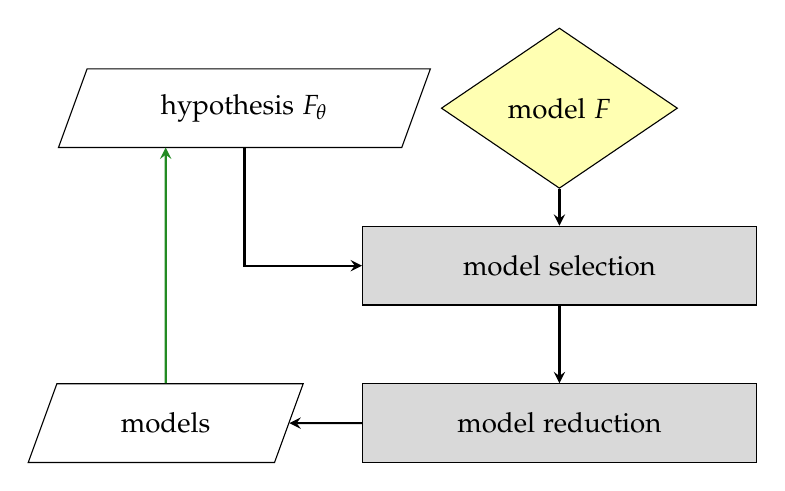
\begin{tikzpicture}[node distance=2cm]

        \node (field) [decision] {model $F$};
        \node (hypothesis) [io, left of=field,  xshift=-2cm] {hypothesis $\rates$};
        \node (parametric) [process, below of=field, minimum width=5cm] {model selection};
        
        \node (decomp) [process, below of=parametric, minimum width=5cm] {model reduction};
        \node (models) [io, left of=decomp, xshift=-3cm] {models};

        \draw [arrow] (field) -- (parametric);
        \draw [arrow] (hypothesis) |- (parametric);
        \draw [arrow] (parametric) -- (decomp);
        
        \draw [arrow] (decomp) -- (models);
        \draw [arrow,color=ForestGreen] (models) -- +(0,3.5);

    \end{tikzpicture}
    \caption{Overview of model selection, reduction and refinement loop}
    \label{fig:non-parametric}
\end{Figure}
Alternatively one may construct $\rates$ to cover a whole class of models rather than a single model \cite{Kuepfer2007EnsembleDynamics}. The expectation is that most of the parameters would be zero but some would be informative \cite{Brunton2016SparseSINDYc}. From the inferred parameters $\theta$ one may construct alternative hypotheses and narrow down the set of plausible models. By iterating this procedure one would identify the minimal model within the model class that explains the data.

\section{Thesis Content Summary}
In this thesis we focus on the benefits of differential equation representations and differentiable \emph{design--learn} workflows in the context of the genetic engineering of cell phenotypes in synthetic biology. In Chapter \ref{chapter:background} we introduce the reader a relevant background in differential equations and machine learning with applications in cell biology to set the stage for the publications in Chapters \ref{chapter:double-exclusive}--\ref{chapter:exploring}. We will see how a differential equation representation of a cell or population of cells requires an exploration of the relationship between bifurcation theory and the concept of a phenotype. Chapter \ref{chapter:double-exclusive} exhibits the results of an interdisciplinary collaboration between in synthetic biology, during which an iterative \emph{design--learn} workflow was followed in an attempt to overcome the biological complexity barrier. During this collaboration, a disconnect between design goals and parameter inference methods was identified which lead to the novel bifurcation inference method published in Chapter \ref{chapter:inference}. Chapter \ref{chapter:exploring} is an adaptation of a publication, in preparation at the time of writing this document, that explores the importance of interactive exploration of high-dimensional flow cytometry data for immunophenotyping. Finally, Chapter \ref{chapter:conclusions} concludes with retrospectives on the previous chapters, which includes a revised view of a \emph{design--learn} workflow for synthetic biology, that in principle is completely differentiable. Furthermore, we propose how one would use concepts from Chapters \ref{chapter:inference}--\ref{chapter:exploring} to interactivity explore the space of hypotheses that represent the same cell phenotype. Our conclusions would be most impactful in cell line development where flow cytometry and other omic-type measurements are taken at different protocol stages of a biomanufacturing process.
\chapter{Theoretical Background}
\label{chapter:background}
\begin{music}
    \parindent10mm \instrumentnumber{1} \setstaffs1{1} 
    \generalmeter{\meterfrac34} \generalsignature{-1}
    \startextract
		\notes  \en
    \zendextract
\end{music}
\epigraph{\textit{the passion of friendship will soon blossom into a righteous power}}{Bolero of Fire --- Ocarina of Time}

% Convolutional neural networks trained on large databases \cite{mnist2012,imagenet2009} have shaped machine learning research over the past couple of decades. Today they serve as canonical learning material in courses and are often used as initial \textit{vanilla} approaches for data exploration and classification tasks and before creating more bespoke machine learning pipelines. The widespread success of much models created an expectation in the research community that with sufficient data and computational power provided by one of the reigning consumer internet businesses, a data-driven black-box model can be created for any application ranging from quantum mechanics to economics. Convolutional architectures together with language models eventually inspired recurrent architectures and attention models where are the key ingredients in the creation of \textit{Alpha Fold} \cite{Jumper2021HighlyAlphaFold} that takes a substantial step towards solving the protein-folding problem. Biotechnology researchers are eager to apply these methods but face the following obstacles

% \begin{itemize}
%     \item \textbf{Insufficient data} due to strategic experimental designs 
%     \item \textbf{Low extrapolation accuracy} for black box-models
% \end{itemize}

This Chapter lays out a background bifurcation theory and machine learning methods relevant to cell biology and flow cytometry. We establish the connection between the concept of phenotypes and bifurcations in Section \ref{section:phenotypes-with-bifurcations} and lay out assumptions and definitions that are used throughout other chapters. Section \ref{section:applications-cell-biology} follows up with concrete applications of differential equations in cell biology and will prepare the reader for the incorporated synthetic biology publication in Chapter \ref{chapter:double-exclusive}.

The problem of inferring phenotypes from data is defined in Section \ref{section:phenotype-inference} with a survey relevant machine learning methods. This section discusses the pre-processing techniques to extract bifurcations from raw data, as has been done in Chapter \ref{chapter:double-exclusive}, and used as a starting point in the incorporated machine learning publication in Chapter \ref{chapter:inference}. Section \ref{section:applications-flow-cytometry} gives the reader a background in flow cytometry and how the machine learning methods discussed in previous sections are used by immunologists to identify immune cell phenotypes. This section lays the foundations for the interactive exploration tool presented in Chapter \ref{chapter:exploring}.

\section{Describing Phenotypes with Bifurcations}
\label{section:phenotypes-with-bifurcations}

%Bringing in the definition here is too early. Too abrupt.
%Historical context of how the word emerged and how it is used in biological contexts
A phenotype is a qualitative state or behaviour of an organism that can be described by several quantitative features. Before considering the additional complexity that comes with biology, let us first consider a simple everyday metaphor: light bulbs. Light bulbs come in various combinations of quantitative features $\theta$ which could be its shape, colour, materials and circuit design. The purpose of a light bulb is to fulfil a single function: increase in brightness as a function of voltage $p$, pushing the qualitative state of the bulb from \emph{off} to \emph{on}. Changes to bulb shape affect neither its function nor its states. Changes in color affect the quality of the \emph{on} state but not the \emph{off} state. Changes to circuit design and materials may change or even break the bulb's function. Fluorescent bulbs, for example, only have two possible brightness states in response to changes in voltage $p$, while incandescent bulbs have a continuous brightness response.
\\
\begin{Figure}
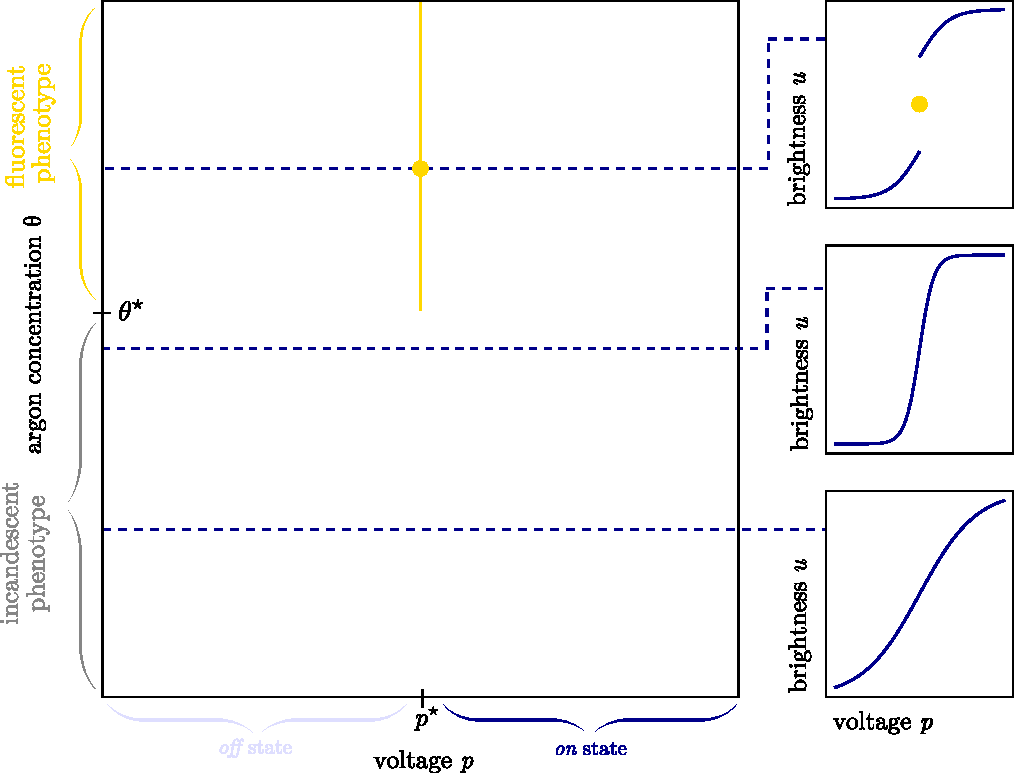
\includegraphics[scale=0.7]{bulb}
\caption{a) The bifurcations (shown in gold) at critical voltage $p^\star$ above argon concentration $\theta^\star$ give rise to sudden jumps in brightness (right-hand panels). $\theta^\star$ separates two bulb phenotypes and $p^\star$ separates the \emph{on} and \emph{off} states.}
\label{fig:bulb}
\end{Figure}

The fluorescent and incandescent bulbs can be considered as two different phenotypes distinguished by the quality of their response to voltage changes. Different colour bulbs can also be considered phenotypes, distinguished by the quality of their \emph{on} state, rather than their response to voltage. Bifurcation theory allows us to describe the transitions between qualitative states and can be leveraged to distinguish and organise phenotypes. In this context a bifurcation becomes a punctuation that either \emph{distinguishes between phenotypes} or \emph{distinguishes between behaviours within a phenotype}.

Suppose we inserted a component into our light bulb that changed parameter $\theta$ in such a way so that we can change between the discrete response of the fluorescent bulb and the continuous response of the incandescent bulb. Perhaps $\theta$ could be the concentration of argon gas; the bulb would have to be wired to behave like an incandescent bulb at low concentrations. We could collect brightness $u$ as a function of voltage $p$ and gas concentration $\theta$ produce something similar to that shown in Figure \ref{fig:bulb}. The bifurcations at critical voltage $p^\star$ above argon concentration $\theta^\star$ give rise to sudden jumps in brightness. The bifurcations separate the \emph{on} and \emph{off} states of the bulb and are only present in the fluorescent phenotype. The two phenotypes lie either side of  the onset of bifurcations at concentration $\theta^\star$. We can see from Figure \ref{fig:bulb} how knowing the locations of bifurcations allows us to organise qualitative behaviours and hence phenotypes of the bulb.

In the biological context, we can consider changes in $\theta$ as changes in the organism genotype that may or may not lead to a new phenotype. The idea of describing phenotypes in this way has been done before by Waddington \cite{}. His epigenetic landscape is a metaphor for how changes gene regulation, in our case represented by changes in $\theta$, determines the fate of cells. He imagines the cell as a marble, rolling down a series of forking valleys representing a differentiation cascade, eventually settling in its final phenotype. Let us adopt this metaphor for organism behaviours in response to a controlled condition (Figure \ref{fig:waddington}). Changing the control condition places the marble at different points in the valley and each fork in the valley corresponds to different available behaviours to the organism. Changing the parameters $\theta$ changes the topology of the valleys potentially giving rise to new behaviours and therefore new phenotypes. Due to the robustness \cite{} and fragility \cite{} of organisms we expect most changes in $\theta$ to either kill the organism or do nothing at all. The emerging picture suggests that the route between phenotypes is a carefully created sequence of changes in $\theta$.

\begin{Figure}
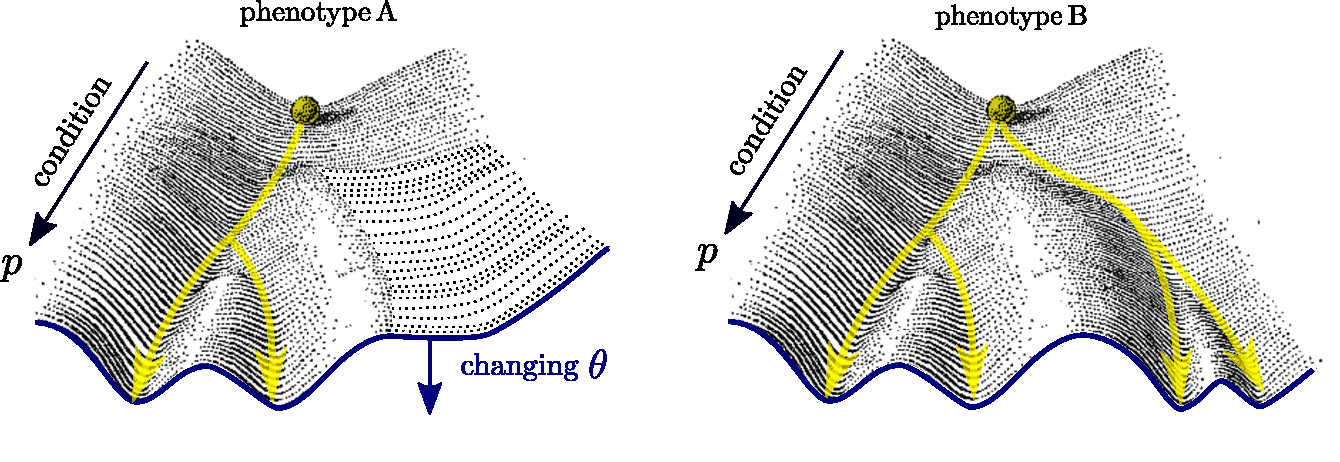
\includegraphics[scale=0.6]{waddington}
\caption{Waddington landscapes representing the set of available behaviours for two phenotypes in response to a controlled condition $p$. Phenotypes are related by changes in landscape topology via changes in $\theta$}
\label{fig:waddington}
\end{Figure}

In order to enumerate the phenotype distribution in the the high-dimensional parameter space $\theta$ for a given organism we can construct a model. By parametrising such a model $\rates(u,p)$ by $\theta$, we can relate the states of the organism $u$ to experimentally controlled conditions $p$. Ideally a subset of $u$ can be observed experimentally so that we may observe bifurcations in the data, as demonstrated in the right-hand panel of Figure \ref{fig:bulb}. In the following section we shall go through a class of models that can leverage bifurcation theory.  

\clearpage
\subsection{Differential Equation Models}

For the purposes of this thesis we will assume that the behaviour of the organism under study can be cast in terms of differential equations in a $N$ states $u$, $M$ parameters $\theta$ and $P$ control conditions $p$. For now we shall state the general class of models and follow up with concrete biological examples as we explore different types of bifurcations. Throughout the thesis we will consider models of the form

\begin{equation}
	\frac{du}{dt} = \rates(u,p)
	\where
	\begin{cases}
		\quad F: \Reals^{N+P}\rightarrow\Reals^N \\
		\quad \theta\in\Reals^M, u\in\Reals^N, p\in\Reals^P
	\end{cases}
	\label{eq:differential-equations}
\end{equation}

\noindent The total derivative $\frac{du}{dt}$ gives us the rate of change of the states with respect to time $t$ and all variables have been vectorised with the appropriate dimension. In principle the right-hand-side $\rates$ can be arbitrarily complicated, containing spatial derivatives or even machine learning models such as neural networks. We shall see later when such models become relevant in biomedical modelling.

\subsubsection{Trajectories \& Field Geometry}

In principle once equations \eqref{eq:differential-equations} have been written down they can be integrated to obtain trajectories $u(t)$ for various initial conditions $u(t')$. We can write the solution down formally as
\begin{equation}
	u(t) = u(t') + \int_{t'}^{t} \rates(u(s),p)\,\mathrm{d}s
	\label{eq:trajectory}
\end{equation}
Here the integral reveals that in order to determine where the state is at time $t$ we need to sum all the contributions of the function $\rates$ from the initial time $t'$ all the way up to final time $t$. The function $\rates$ depends on the state $u$ and must be updated with the integration variable $s$. This calculation can be interpreted, as shown in Figure \ref{fig:fields}, as choosing an initial point $u'=u(t')$ in a vector field $\rates$ and following the field lines until time $t$ at which the final point $u=u(t)$ has been reached.

\begin{Figure}
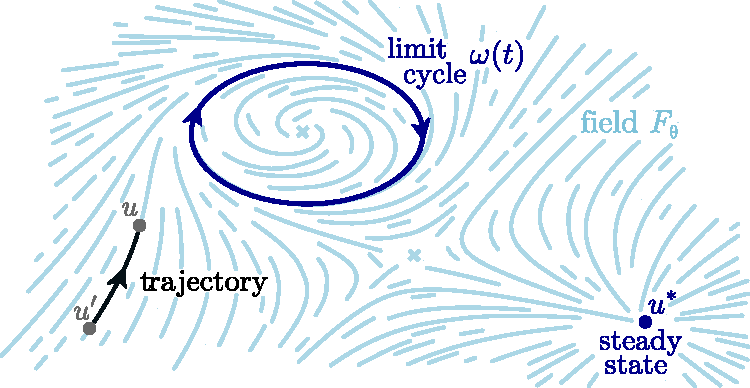
\includegraphics[scale=0.9]{fields}
\caption{Illustration of a trajectory between $u=u(t)$ and $u'=u(t')$ over finite time $t-t'$ following the field lines of $\rates$. In this example field lines either point towards steady state $\steady$ or a limit cycle $\cycle(t)$. There are two unstable fixed points marked by crosses: a saddle point separating the basins of attraction and an unstable focus enclosed by the limit cycle.}
\label{fig:fields}
\end{Figure}

By considering the geometry of the field $\rates$ in state space we can determine the fate of sets of trajectories, which are ultimately pulled towards \emph{dynamical attractors}. Such attractors can be static steady states $\steady$ or dynamic like the limit cycle $\cycle(t)$ illustrated in Figure \ref{fig:fields}. \emph{Dynamical attractors} create basins of attraction defined as regions of state space in which trajectories are pulled towards the same stable structure. These basins must be separated by unstable structures, such as the saddle point marked by a cross in Figure \ref{fig:fields}, which define a boundary between the basins called the separatrix. Note that the direction of the field $\rates$ and not its magnitude $|\rates|$ determines the fate of a trajectories.

When equations \eqref{eq:differential-equations} describe the behaviours of an organism, the attractors determine the set of qualitative behaviours available to the organism of genotype $\theta$, whilst experiencing experimental conditions $p$. If changes to the genotype $\theta$ change the number, type or stability of the attractors then we will observe new qualitative behaviours and hence a new phenotype. If changes to conditions $p$ lead to changes in the state space geometry, this is interpreted as a different behavioural state available to the same phenotype. We can see therefore how casting a biomedical problem into the language of differential equations, allows us to characterise phenotypic traits with the geometry of attractors in state space. 

\subsubsection{The Jacobian Matrix}

In order to quantify the geometry of a local patch of state space $u$ we can imagine $\rates$ as a velocity field of water and place a tiny blob of ink surrounding the location $u$. The so called Jacobian matrix $\jacobian$ of partial derivatives at the location $u$ transforms the basis vectors $\hat u(t)$ defining the blob over a short period of time $\Delta t$ as depicted in Figure \ref{fig:jacobian}. The transformation is
\begin{equation}
	\hat{u}(t+\Delta t)=\left (\mathbb{1}+\jacobian\Delta t \right)\hat{u}(t)
	\where
	\hat{u}\in\Reals^N\quad
	\jacobian\in\Reals^{N\times N}
	\label{eq:jacobian-transformation}
\end{equation}

\begin{Figure}
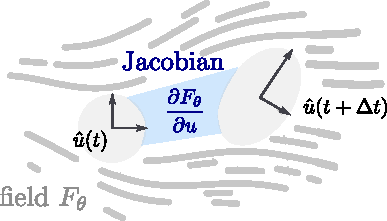
\includegraphics[scale=1.2]{jacobian}
\caption{Illustration how the Jacobian matrix $\jacobian$ transforms the basis vectors $\hat u(t)$ defining a small patch of initial conditions for a short period of time $\Delta t$. The eigenvalues $\lambda$ and eigenvectors $\eigenvector$ define the deformation of the patch}
\label{fig:jacobian}
\end{Figure}
\noindent where $\mathbb{1}$ is the identity matrix. The eigenvalues $\lambda$ and eigenvectors $\eigenvector$ of the Jacobian reveal to us the magnitudes and directions of the stretching or squeezing of the blob. We can diagonalise the Jacobian to obtain the eigenvalues and eigenvectors at any state space location $u$ to quantify the local geometry of the field. The eigenvalue equation is written as

\begin{equation}
	\lambda \eigenvector = \jacobian\eigenvector
	\where
	\eigenvector\in\Reals^N : |\eigenvector|=1
	\label{eq:jacobian-eigenproblem}
\end{equation}
where the eigenvectors are normalised to have unit magnitude. We can take the limit $\Delta t\rightarrow 0$ of equation \eqref{eq:jacobian-transformation} to obtain a first order matrix differential equation for the evolution of basis vectors $\hat u(t)$ in any patch $u$
\begin{equation}
	\frac{d\hat{u}}{dt}=\jacobian\hat{u}
	\label{eq:jacobian-odes}
\end{equation}
The coefficients given by the Jacobian matrix are time-independent and therefore the general solution can be written as a matrix exponential
\begin{equation}
	\hat{u}(t)=\e^{\jacobian(t-t')}\hat{u}(t')
	\label{eq:basis-vector-evolution}
\end{equation}
where $\hat{u}(t')$ are the basis vectors that define the initial shape of the blob centred on location $u$. If we let the basis for the initial blob be parallel to the eigenvectors $\eigenvector$ of the Jacobian, then the evolution any vector $\sigma(t)$ within the blob expressed in its basis becomes the linear superposition
\begin{equation}
	\sigma(t)= \sum_{\lambda}\eigenvector
	\sigma_{\lambda}(t') \e^{\lambda(t-t')}
	\label{eq:eigenbasis-vector-evolution}
\end{equation}
where $\sigma_{\lambda}(t')$ are the initial components of the vector in the basis of the blob. This equation reveals explicitly how the sign of real parts to eigenvalues $\Real\lambda$ determine the exponential growth or shrinkage of the blob in the direction $\eigenvector$. The imaginary parts $\Imag\lambda$ determine the magnitude of rotations of the blob. Note that since the Jacobian matrix is real and eigenvalues and eigenvectors appear in conjugate pairs and therefore the overall evolution \eqref{eq:eigenbasis-vector-evolution} yields real transformations of blob vectors $\sigma(t)$. The transformation \eqref{eq:jacobian-transformation} an approximation of the time-ordered exponential transformation \cite{} and we should note that the results stated here are valid for small blobs $|\sigma(t)|\ll 1$ over short timescales $|t-t'|\ll1$.

\subsubsection{Time Ordered Exponetials}

In this section we go a bit deeper into the origin of transformation \eqref{eq:jacobian-transformation} for those who are interested the evolution of state space blobs over arbitrary time intervals. We begin by considering the evolution of the separation between a trajectory $u(t)$ and its perturbation $u(t)+\delta u(t)$
\begin{equation}
	\frac{d}{dt}(u+\delta u) = \rates(u+\delta u,p)
\end{equation}
After Taylor expanding the field $\rates$ and recognising that equations \eqref{eq:differential-equations} lead to a cancellation in the terms involving the unperturbed trajectory $u$ we arrive at
\begin{equation}
	\frac{d}{dt}(\delta u) =
	\left.\jacobian\right|_{u=u(t)}\!\!\delta u + \mathcal{O}(\delta u^2)
	\label{eq:linearised-differential-equations}
\end{equation}
where $\jacobian$ is the Jacobian of the field and additional terms $\mathcal{O}(\delta u^2)$ involve taking higher order derivatives of the field $\rates$. Choosing a perturbation sufficiently small such that we can ignore higher order terms yields a first order homogenous ordinary matrix differential equation of the form $\dot{\delta u}(t)\approx J(t)\delta u(t)$ where $J(t)$ is a time-varying Jacobian. These equations can be solved formally with time-ordered matrix exponentiation \cite{} 

\begin{Figure}
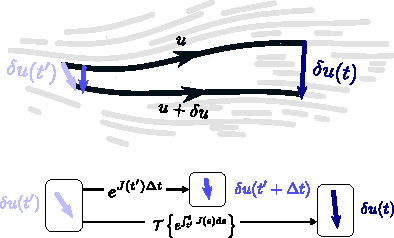
\includegraphics[scale=1.5]{lyapunov}
\caption{Illustration how the time ordering operator $\mathcal{T}\left\{\e^{\int_{t'}^t J(s) \mathrm{d}s}\right\}$ propagates the separation $\delta u(t)$ between adjacent trajectories $u$ and $u+\delta u$ by repeated application of the exponentiated Jacobian $\e^{J(t)\Delta t}$ evaluated along trajectory $u(t)$}
\label{fig:lyapunov}
\end{Figure}
\begin{equation}
	\delta u(t) \approx
	\mathcal{T}\left\{\e^{\int_{t'}^t J(s) \mathrm{d}s}\right\}\delta u(t')
	\where
	J(t) := \left.\jacobian\right|_{u=u(t)}
	\label{eq:matrix-exponential}
\end{equation}
The time-ordering defines an ordered product of matrix exponentials
\begin{equation}
	\mathcal{T}\left\{ \e^{\int_{t'}^t J(s) \mathrm{d}s} \right \}:=
	\lim_{\Delta t\rightarrow 0}\left(
		\e^{J(t)\Delta t}\e^{J(t-\Delta t)\Delta t}\,\dots\,
		\e^{J(t'+\Delta t)\Delta t}\e^{J(t')\Delta t}
	\right)
	\label{eq:time-ordering-operator}
\end{equation}
which can be calculated by repeated exponentiation of the Jacobian $\e^{J(t)\Delta t}$ evaluated at different times along the unperturbed trajectory $u(t)$. Although this expression may look complicated it is just another matrix whose eigenvalues reveal whether the trajectories diverge $|\delta u(t\rightarrow\infty)|\rightarrow\infty$ or converge $|\delta u(t\rightarrow\infty)|\rightarrow0$.

In situations where we want to investigate field flow over longer time intervals or where there is an explicit time dependence in the field $\rates(u,p,t)$ we must use the time-ordered exponential \eqref{eq:time-ordering-operator} in place of the exponentiated Jacobian.

\subsubsection{Lyapunov Exponents}
Sometimes we are only interested in the rate of change of the magnitude of deformations $|\sigma(t)|$ which can quantified by the \emph{finite time lyapunov exponent}
\begin{equation}
	\Lambda(u,\Delta t):=\frac{1}{\Delta t}\log\frac{|\sigma(t+\Delta t)|}{|\sigma(t)|}
\end{equation}
We remind ourselves that the blob $\sigma(t)$ is centred around state space point $u$, then evolved for a time $\Delta t$ and therefore the exponent is a function of $\Delta t$ and $u$. Substituting equation \eqref{eq:eigenbasis-vector-evolution} we arrive at
\begin{equation}
	\Lambda(u,\Delta t) = \frac{1}{2\Delta t}\log
	\left\langle
		\e^{2\Real[\lambda]\Delta t}
	\right\rangle_{\sigma(t)}
	\ge 
	\left\langle
		\Real[\lambda]
	\right\rangle_{\sigma(t)}
	\label{eq:finite-time-lyapunov}
\end{equation}
where $\left\langle\cdots\right\rangle_{\sigma(t)}$ is a shorthand for a weighted arithmetic average over the components of the initial blob $\sigma(t)$. We have used Jensen's Inequality \cite{} to show that the rate of distortions is bounded by the average of real parts of eigenvalues. This bound becomes an equality for eigenvalue $\lambda$ when the blob $\sigma(t)$ is initialised along only its eigenvector $\eigenvector$. We will see later how the \emph{Lyapunov exponents} are useful for extracting timescales around interesting structures in state space such as \emph{fixed points} and \emph{degeneracies}. 

\subsubsection{Fixed Points}

Thus far we explored the field geometry in arbitrary patches of state space $u$ and asked questions about local flows. It is usually not possible to set up experimental conditions to get an organism to trace out all of its available states without killing it or distorting the mechanism under study. An organisms prefers to operate within a finite set of states and would want to return to them when perturbed. In biology this is known as \emph{homeostasis} and in the context of dynamical systems this is a stable steady state $\steady$ which belongs to a wider class of points called \emph{fixed points}. In the context of differential equation models, a \emph{fixed point} is the solution of
\begin{equation}
	\left.\frac{du}{dt}\right|_{u=\steady}=\rates(\steady,p) = 0
	\label{eq:fixed-point-equation}
\end{equation}

\begin{Figure}
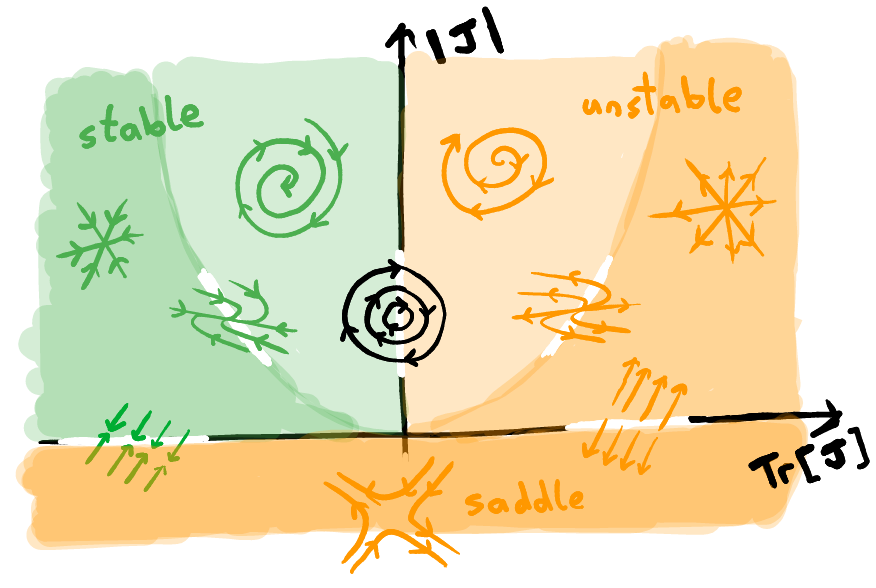
\includegraphics[scale=0.35]{stability}
\caption{Classification of stable and unstable fixed points for a general two dimensional systems in terms of trace $\mathrm{Tr}[\jacobian]$ and determinant $|\jacobian|$ of its Jacobian}
\label{fig:stability}
\end{Figure}

By looking at the eigenvalues of the Jacobian, which determine local flows according to equations \eqref{eq:eigenbasis-vector-evolution}, we can classify the fixed point $\steady$. The sign of real parts $\Real\lambda$ determine whether small perturbations away from the fixed point will diverge. This defines whether the point is \emph{stable}, \emph{unstable} or a \emph{saddle}. Non-zero imaginary parts $\Imag\lambda \ne 0$ give rise to damped oscillation around the point; these points are called \emph{foci}. Without real parts the flow becomes purely rotational and give rise to \emph{cycles}.

For a two dimensional system we can express the two eigenvalues of the $2\times 2$ Jacobian in terms of its trace $\mathrm{Tr}[\jacobian]$ and determinant $|\jacobian|$ which allows us to conveniently reveal all the possible fixed points types, as in Figure \ref{fig:stability}. If at least one the eigenvalues vanishes the fixed point becomes \emph{degenerate}. We shall see that \emph{degenerate} field flows lead to critical slowing down in dynamics, reveal bifurcations and are useful for constructing tangent fields to implicitly defined surfaces.

\subsubsection{Field Degeneracy}
A field $\rates$ can be called \emph{degenerate} where it is locally constant and hence does not cause shape changes to a blob of initial conditions in one or more directions. This means that one or more of the eigenvalues of the Jacobian vanish $\lambda = 0$ and have associated eigenvectors $\hat T_\lambda$ tangent to the direction where the field is locally constant. Suppose the field is \emph{degenerate} at point $\degenerate$, then the vanishing eigenvalues lead to a zero determinant $\left|\jacobian\right|=0$ and the eigenvectors must be orthogonal to all the gradients
\begin{equation}
	\left|\jacobian\right|_{u=\degenerate} \!\!\! = 0
	\qquad\left.\jacobian\right|_{u=\degenerate}\!\!\!\hat T_\lambda = 0
	\where
	\hat T_\lambda\in\Reals^N : |\hat T_\lambda|=1
	\label{eq:degeneracy-conditions}
\end{equation}
The eigenvector equation yields $\hat T_\lambda$ that span the degenerate subspace at field location $\degenerate$. The number of vectors and hence the size of the subspace is given to us by the number of vanishing eigenvalues $\lambda=0$. In linear algebra this would be referred to as the \emph{nullspace} or \emph{kernel} of the Jacobian matrix. A vanishing determinant means that the Jacobian is not invertible.

\subsubsection{Critical Slowing Down}
% A fixed point $\steady$ that is also degenerate $\degenerate$ is called a critical point $\critical$. This is a location in the state space that satisfies equations \eqref{eq:fixed-point-equation} and \eqref{eq:degeneracy-conditions}. This means that the field $\rates$ is not only zero, but also locally zero along at least one direction. In this case the whole degenerate subspace takes on the character of the fixed point and gives rise to power law timescales that are characterised using \emph{critical exponents}.

% \emph{Critical exponents} are not the same as \emph{Lyapunov exponents} although we will see that they are related. These exponents are important because the power laws can be detected in trajectory data and can be used to classify bifurcations.

Lets us consider the magnitude of deformations along the degenerate direction $T_\lambda(t)$ in the vicinity of the the region $u\approx\degenerate$ that is driven by the scalar sub-field $F_\lambda$. We expect the first-order derivatives to vanish $\left.\frac{dF_\lambda}{dT_{\lambda}}\right|_{u=\degenerate}\!\!\!\!\!\!\!\!\!\!\!\!\!\!\!=0$ and therefore have to expand the field $F_\lambda$ to an order $n$ that will yield the first non-zero derivative. The equations expanded for $u\approx\degenerate$ are
\begin{align}
	\frac{d T_\lambda}{dt} &= \left.\frac{dF_\lambda}{dT_{\lambda}}\right|_{u\approx\degenerate}
	\!\!\!\!\!\!\!\!\!\!\!\!T_\lambda(t) +
	\frac{1}{n!}
	\left.\frac{d^n F_\lambda}{dT_{\lambda}^n}\right|_{u\approx\degenerate}
	\!\!\!\!\!\!\!\!\!\!\!\!T_{\lambda}(t)^n +\mathcal{O}(T^{n+1})
	\where n \ge 2
	\label{eq:bernoulli-differential-equation}
\end{align}
Here we kept the first-order derivative because we would still like to see how the dynamics scales with time as we approach to degeneracy. This is a Bernoulli differential equation \cite{} with constant coefficients and has a general solution
\begin{align}\!\!\!\!\!
	T_{\lambda}(t) = \left(
	\left(T_{\lambda}(t')\e^{(t-t')
	\left.\frac{dF_\lambda}{dT_{\lambda}}\right|_{u\approx\degenerate}
	}\right)^{1-n}
	-(t-t')\frac{n-1}{n!}\left.\frac{d^n F_\lambda}{dT_{\lambda}^n}\right|_{u\approx\degenerate}
	\right)^{\frac{1}{1-n}}
	\label{eq:critical-slowing}
\end{align}

This equation reveals two timescales for blob deformations in the vicinity of a field degeneracy: the familiar exponential timescale $\e^{t-t'}$ and a new polynomial timescale $(t-t')^{\frac{1}{1-n}}$. The emergence of a polynomial timescale that dominates over the exponential is called \emph{critical slowing down} and is a marker of degeneracy. We can see once the dynamics is confined to the degenerate subspace the eigenvalues of the Jacobian are insufficient for determining the timescales. The curvature of the field around the degenerate subspace drives the polynomial dynamics, and therefore higher-order derivatives are needed to reveal this.

This critical slowing can be observed in data when \emph{fixed points} become \emph{degenerate}. Degenerate fixed points are also called \emph{critical points}. The transition between these two timescales in data is a signal that a \emph{critical point} is nearby. We will see that \emph{critical points} may lead to bifurcations and bifurcations are always accompanied by degeneracies in the field.

\subsubsection{Fluctuations}

Biological processes can be intrinsically noisey and the measurement apparatus can also introduce errors. Fortunately we can model such non-deterministic aspects by extending equations \eqref{eq:differential-equations} to a Langevin equation
\begin{align}
	\frac{du}{dt} = \rates(u,p) + \eta(t)
	\where \eta(t) \sim \mathcal{N}(\mu=0,\mathbf{\Sigma}=\mathbb{1}D)
	\label{eq:langevin}
\end{align}
The stochastic process $\eta(t)$ is a zero-mean white noise with equal variance $D$ along all $N$ dimensions resultant from a large number of independent processes such as Brownian motion and Poisson shot noise. We can apply the Kramers-Moyal expansion \cite{} to transform this equation into an equivalent Fokker-Planck equation for the probability distribution $P_{\theta}$
\begin{align}
	\frac{dP_{\theta}}{dt} + \frac{\partial}{\partial u}\cdot J_\theta = 0
	\where J_\theta := \left(\rates(u,p)-\frac{D}{2}
	 \frac{\partial}{\partial u} \right)P_{\theta}
	\label{eq:fokker-planck}
\end{align}
Here we cast the Fokker-Planck equation as a continuity equation with the divergence of probability current $J_\theta$ balancing the total change in probability $\frac{dP_{\theta}}{dt}$. In the scenario where at steady state $\frac{dP_{\theta}}{dt}=0$ there are also no circulating probability currents $J_\theta=0$ then we can solve for the distribution
\begin{align}
	P_{\theta}(u,p) = \frac{1}{Z} \mathbb{e}\,^{\frac{2}{D}\int^{u}\!\!\!\rates(u',p)\cdot\mathrm{d}u'}
	\where Z:= \int_{\Reals^N} \mathbb{e}\,^{\frac{2}{D}\int^{u}\!\!\!\rates(u',p)\cdot\mathrm{d}u'} \mathrm{d}u
	\label{eq:steady-state-distribution}
\end{align}
Expanding the distribution in the vicinity of a stable fixed point gives rise to a multivariate Gaussian distribution whose covariance matrix $\mathbf{\Sigma}$ is the inverse of the Jacobian evaluated at the fixed point
\begin{align}
	P_{\theta}(u,p) \sim \mathbb{e}\,^{-\frac{1}{2}
	(u-\steady)^\top\mathbf{\Sigma}^{-1}(u-\steady)
	}\where \mathbf{\Sigma}^{-1}=-\frac{2}{D}\left.\jacobian\right|_{\steady}
	\label{eq:steady-state-distribution-near-fixed-point}
\end{align}
We learn that accompanying the \emph{critical slowing down} \eqref{eq:critical-slowing} we also have the divergence of variance along the degenerate direction. These are the two main observations that accompany bifurcations and have a deep relationship to the theory of phase transitions \cite{}.

\subsubsection{Limit Cycle Analysis}
Thus far we dealt with static state space structures like \emph{fixed points}. We found that the eigenvalues of the Jacobian are sufficient for their characterisation, unless the field is  \emph{degenerate}, in which case higher order derivatives of the field must be investigated.

If fields lines point towards a region of state space but the region \emph{does not} contain any fixed points, then the only other option is for the field lines to converge onto a \emph{limit cycle}. This is actually a rough statement of the Poincar\'e-Bendixson theorem  which allows us to define trapping regions where trajectories do not escape from and make statements about the existence or non-existence of limit cycles. A limit cycle must also enclose a finite number of \emph{unstable foci} that push trajectories away from its center.

Newton-type methods can easily be applied to find \emph{fixed points} because they are local structures in fields. Limit cycles are much more tricky because it is not possible to know whether a local state part of a limit cycle or not before we have seen a trajectory visit that state twice: once at $u(t)$ and then again $u(t+T)$ after some time $T$. This forms the basis of some optimisation methods for computing limit cycles \cite{}.

\begin{itemize}
	\item Trapezoid method
	\item Collocation method
	\item Shooting method
\end{itemize}

% \begin{Figure}
% 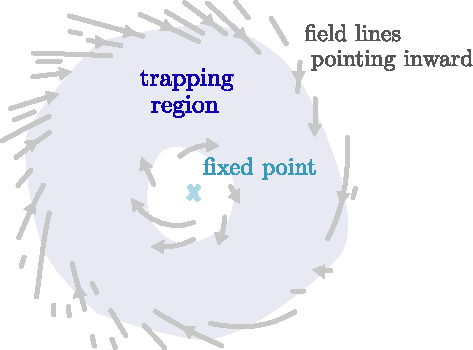
\includegraphics[scale=0.35]{limit-cycle}
% \caption{}
% \label{fig:limit-cycle}
% \end{Figure}

\clearpage
\subsection{Bifurcation Analysis}
\label{section:bifurcation-analysis}
We have surveyed sufficiently many state space structures, the geometry of which determine the qualitative behaviour of the organism we are describing. An organism has many qualitative behaviours in response to conditions $p$ and many phenotypes emerging from changes in $\theta$.

Bifurcations are defined as qualitative changes to system behaviour in response to smooth changes to some conditions. In our setting these conditions could be either $\theta$ or $p$, but we will focus on changes with respect to $p$ with the understanding that the analysis is equally valid for $\theta$. We are ready to present the two \emph{generic} and \emph{robust} one parameter bifurcations: the \emph{saddle-node} and \emph{Hopf} bifurcation. These bifurcations are generic in the sense that they happen in $N$ dimensional systems, but can be described as happening along one dimension. This is true because of centre manifold theory \cite{}. The bifurcations are \emph{robust} in the sense that small changes to system parameters do not destroy the bifurcation. This is not the case for \emph{pitchfork} and \emph{transcritical} bifurcations which we will present in a separate section.
\subsubsection{Generic Robust Bifurcations}
\begin{Figure}
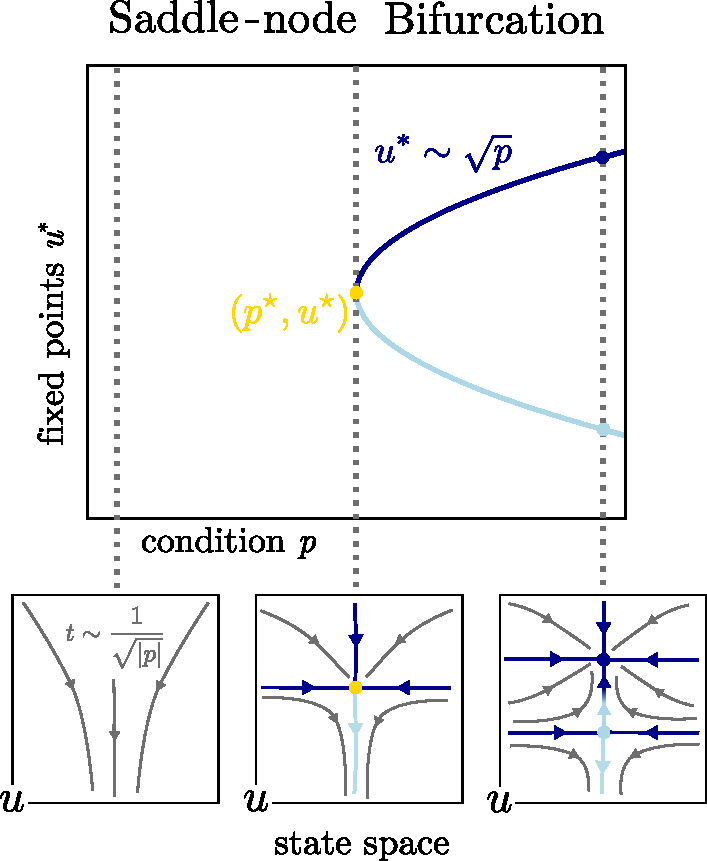
\includegraphics[scale=0.6]{saddle-node} 
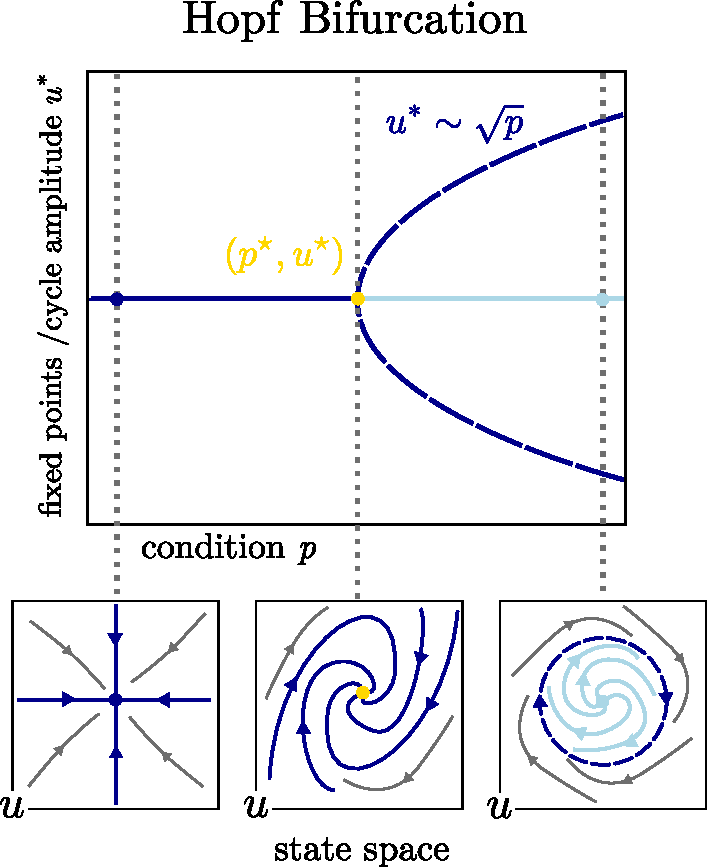
\includegraphics[scale=0.6]{hopf}
\caption{Generic and robust bifurcations. A. \emph{Saddle-node} bifurcations create or annihilate stable and unstable pairs of fixed points. B. In \emph{Hopf} bifurcations a stable fixed point becomes an unstable focus that pushes trajectories towards a limit cycle.}
\label{fig:robust-local-bifurcations}
\end{Figure}
\subsubsection{Fragile Bifurcations}
\begin{Figure}
	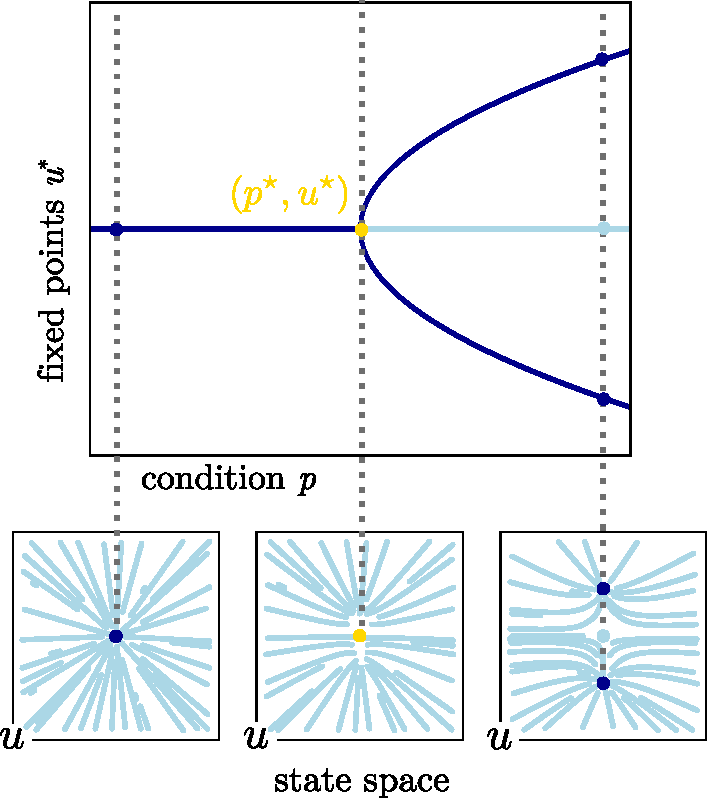
\includegraphics[scale=0.6]{pitchfork}
	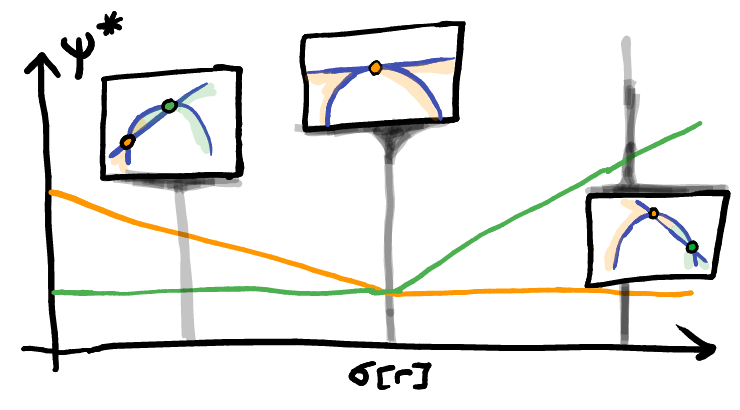
\includegraphics[scale=0.6]{transcritical}
	\caption{Fragile bifurcations}
	\label{fig:fragile-bifurcations}
\end{Figure}
\subsubsection{Global Bifurcations}
\begin{Figure}
	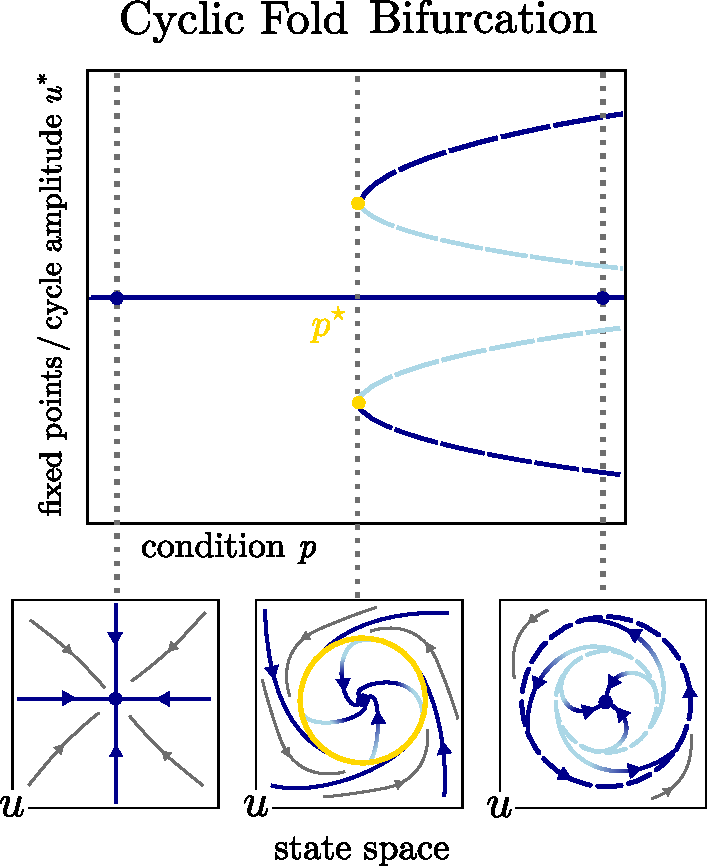
\includegraphics[scale=0.6]{cyclic-fold}
	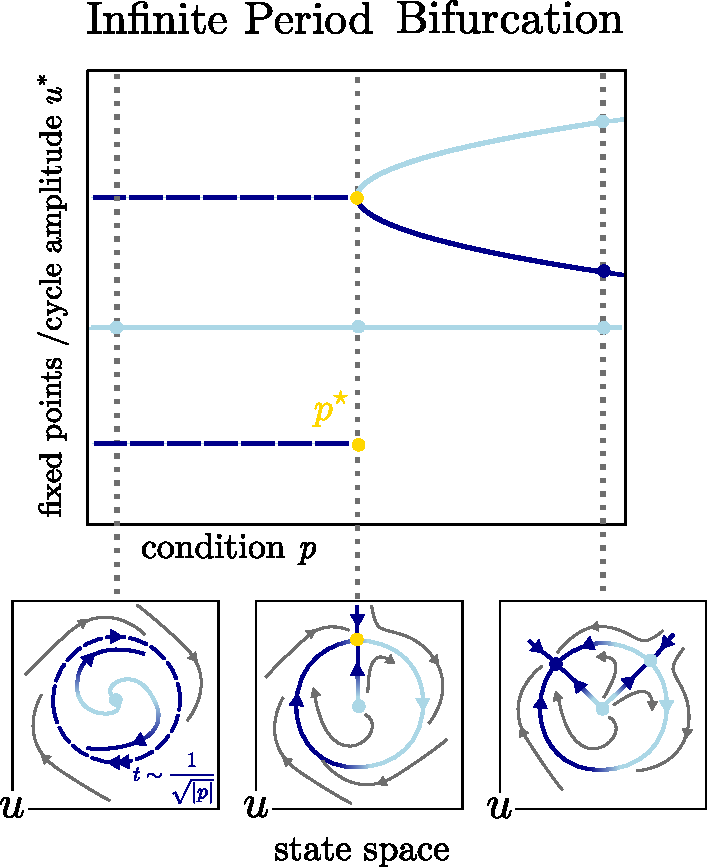
\includegraphics[scale=0.6]{infinite-period}
	\caption{Global Bifurcations}
	\label{fig:global-bifurcations}
\end{Figure}

\begin{Figure}
	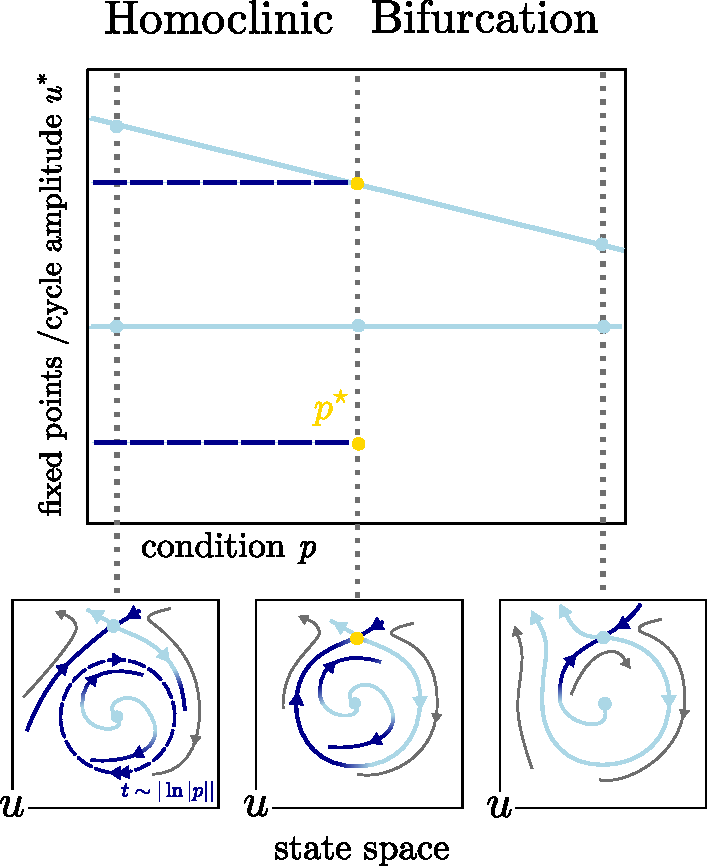
\includegraphics[scale=0.6]{homoclinic}
	\caption{Homoclinic Bifurcation}
	\label{fig:homoclinic}
\end{Figure}

\subsubsection{Higher Co-dimension}
\begin{itemize}
	\item cusp and Bogdanov-Takens
	\item centre manifold theory
\end{itemize}

\subsubsection{Numerical Methods}

In this thesis we extensively use the library \texttt{DifferentialEquations.jl} \cite{Rackauckas2017Differentialequations.jlJulia} for numerically solving differential equations and \texttt{BifurcationKit.jl} \cite{Veltz2020BifurcationKit.jl} for calculating bifurcation diagrams. 

\begin{itemize}
	\item Parameter Continuation
	\item Marching cubes
\end{itemize}

\subsection{Spatially Extended Systems}

If $\rates$ contains spatial derivatives, additional conditions on $u$ with respect to spatial variables $x\in\Reals^D$, where $D$ is the dimension of the space considered, must be supplied to give a unique solution $u(x,t)$. When studying spatio-temporal dynamics of organisms, a popular choice is to incorporate a diffusive term that models the exchange of matter between spatial locations

\subsubsection{Turing Bifurcations}

Here we first introduce diffusion macroscopically by simply adding the laplacian
to mean field equation. We introduce the turning bifurcation and
show how linear stability analysis is insufficient to capture pattern formation
and rich inhomogeneous steady states. A promising approach may be geometrisation
of the moving local equilibria \cite{Halatek2018}.

\clearpage
\section{Applications in Cell Biology}
\label{section:applications-cell-biology}

In this section we apply the dynamical systems theory outlined in Section \ref{section:phenotypes-with-bifurcations} to concrete biochemical systems and provide the reader with sufficient background to understand the goals of the incorporated publication in Chapter \ref{chapter:double-exclusive}.

\subsection{Genetic Switches \& Phenotype Boundaries}
Every cell belonging to an organism has essentially the same genetic information inside it. In spite of this, a wide variety of cell populations such as neurons, muscle cells, immune cells and tissue specific cells interact in a highly regulated fashion. As an organism develops, how do cells which used to be identical differentiate into functionally distinct populations? How are boundaries between these populations maintained? Can these boundaries be controlled with genetic engineering? 

In order to address these questions the paradigm of the \emph{genetic switch} emerged. Genes are either expressed into proteins or not. The concentration of proteins within a cell and on its membrane determine its function and communication abilities with other cells. The genes that are turned \emph{on} or \emph{off} when a cell is exposed to different environments determine the cell phenotype. Genes switching between \emph{on} and \emph{off} in response to other genes or proteins is called \emph{gene regulation}.

The first gene regulatory network that was discovered is the \emph{lac operon} in the bacterium \emph{Escherichia coli} \cite{Jacob1961GeneticProteins}. In this network, enzymes that metabolise lactose are expressed only in the presence of lactose and absence of glucose. This regulation evolved because metabolising lactose is energetically more expensive and having the \emph{lac} genes always turned \emph{on} would be a waste of resources. An outline of how this network works is shown with in Figure \ref{fig:lac-operon}. The main proteins involved in this mechanism are the \emph{Lac Repressor} and $\beta$-\emph{galactosidase} which are transcribed and translated from the \emph{LacI} and \emph{LacZ} genes respectively. The repressor binds to the operator which sits between the promoter and coding region \emph{LacZ}. When the transcription machinery binds to promoter region, it is blocked from transcribing \emph{LacZ}. When lactose is present, binding to the repressor causes a conformational change which leads to unbinding of the complex from the DNA. Thus in the presence of lactose, \emph{LacZ} is turned \emph{on} and $\beta$-\emph{galactosidase} is produced by the cell. In this setting lactose is referred to as the \emph{effector}. We note that the effector of \emph{LacZ} is actually \emph{allolactose} which arises from the transglycosylation of lactose by $\beta$-\emph{galactosidase} but for the purposes of introducing the genetic switch we need not focus in this detail. $\beta$-\emph{galactosidase} hydrolyses lactose, breaking it down into glucose and galactose which decreases the overall concentration of lactose available to bind to the repressor. Eventually all the lactose is is broken down and the repressors turn \emph{off} the \emph{LacZ} gene.

\begin{Figure}
	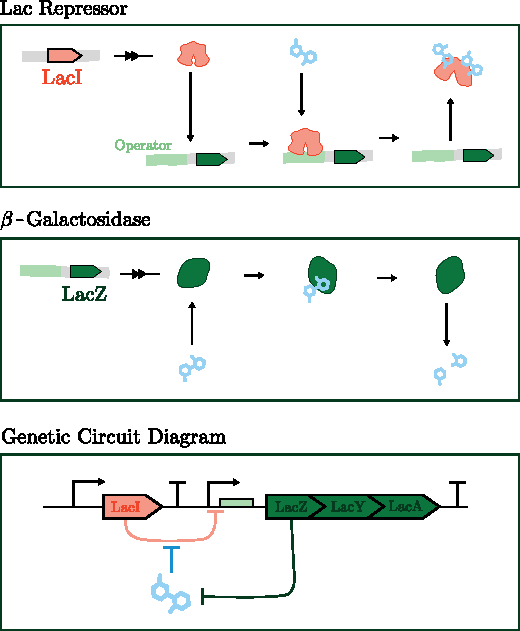
\includegraphics[scale=0.9]{lac-operon}
	\caption{Overview of the \emph{lac operon} }
	\label{fig:lac-operon}
\end{Figure}

Let us first consider what happens within a single cell of constant volume. We assume the rate $\alpha$ of transcription and translation of \emph{LacZ} into $\beta$-Gal is constant unless the operator region is blocked by \emph{LacR}. The repressor is inactivated by the binding of two (allo)lactose molecules $\ce{C12H22O11}$.

\begin{align*}
	\ce{
	\bond{~}Operator\bond{~}LacZ\bond{~} &->[$\alpha$]
	\bond{~}Operator\bond{~}LacZ\bond{~} + $\beta$-Gal \\
	C12H22O11 &->[$\beta$-Gal][+H2O] C6H12O6 + C6H12O6 \\
	\bond{~}Operator\bond{~}LacZ\bond{~} + LacR &<=>[k] \bond{~}Operator^\prime\bond{~}LacZ\bond{~} \\
	LacR + 2C12H22O11 &<=>[k^\prime] LacR^\prime}
\end{align*}
Proteins degrade over some finite half-life $\mu$ we also have
\begin{align*}
	\ce{$\beta$-Gal ->[$\mu$] \emptyset}
\end{align*}

The equilibrium dissociation constants $k,k'$ define the binding affinity if \emph{LacR} to the operator and its effector respectively. Let rate $\beta$ be the rate of hydrolysis of lactose by $\beta$-Gal. These rates are determined by molecular details, some of which can be modulated with genetic engineering. Changing the promoter sequences, for example, can modulate the rate $\alpha$. Thus it makes sense to collect these rates into our model parameter $\theta=(\alpha,\beta,k,k')$. Let the concentration of the effector be the experimentally controlled condition $p=[\ce{C12H22O11}]$ and the remaining concentrations be collected in state vector $u=(\mathrm{LacZ},\mathrm{LacR},\mathrm{Gal})$.

From this set of reactions it is possible to write down a \emph{chemical master equation} \cite{Gillespie1992,Gillespie2007} whose \emph{mean field approximation} yields a set of ordinary differential equations of the form \eqref{eq:differential-equations} which are commonly referred to as \emph{reaction rate equations}. This procedure is equivalent to the mass-action assumption used in chemistry. We note that the two major assumptions here are: a thermodynamic limit where the number of molecules is sufficiently large such that correlations due to discreteness can be ignored and a sufficiently \emph{well mixed} cytoplasm so that we do not have to model space.

The \emph{reaction rate equations} for the Lac operon become
\begin{align}
\frac{d}{dt}\mathrm{LacR} =  \mathrm{LacR}^\prime-& \frac{p^2}{2} k^{\prime} \mathrm{LacR} +  \mathrm{LacZ}^\prime  - k \mathrm{LacR}\,\mathrm{LacZ} \label{eq:lacR}\\\nonumber
\frac{d}{dt}\mathrm{LacR}^\prime =  -  &\mathrm{LacR}^\prime + \frac{p^{2}}{2} k^{\prime} \mathrm{LacR} \\\nonumber\\
\frac{d}{dt}\mathrm{LacZ} = & \mathrm{LacZ}^\prime - k \mathrm{LacR}\,\mathrm{LacZ}
\label{eq:lacZ}\\\nonumber
\frac{d}{dt}\mathrm{LacZ}^\prime =  - & \mathrm{LacZ}^\prime + k \mathrm{LacR}\,\mathrm{LacZ} \\\nonumber\\
\frac{d}{dt} \mathrm{Gal}= &\alpha \mathrm{LacZ} - \mu\mathrm{Gal}\label{eq:Gal} \\\nonumber
\frac{dp}{dt} = 2 \mathrm{LacR}^\prime &-p^{2} k^{\prime} \mathrm{LacR} - \beta p\,\mathrm{Gal} 
\end{align}
We can see two mass conservations: the total concentration of the $\mathrm{LacZ}$ gene and total concentration of $\mathrm{LacR}$. We can write down the conservation laws normalised such that the total concentrations add up to one
\begin{align}
	\mathrm{LacR}+\mathrm{LacR}^\prime + \mathrm{LacZ}^\prime &=1
	\label{eq:mass-conservation}\\\nonumber
	\mathrm{LacZ}+\mathrm{LacZ}^\prime =1 &
\end{align}
Substituting conservation laws \eqref{eq:mass-conservation} into equations \eqref{eq:lacR} and \eqref{eq:lacZ} allows us to close them and solve for the fraction of unbound $\mathrm{LacZ}$ available for transcription
\begin{align}
	\mathrm{LacZ}(p) = \frac{1}{\frac{1}{2}+\sqrt{\frac{1}{4}+\frac{k}{1+\frac{1}{2}k^\prime p^2}}}
	\label{eq:lac-unbound}
\end{align}
This is a \emph{hill}-type term that yields a basal level of transcription $\mathrm{LacZ}(p=0)\sim k^{-\frac{1}{2}}$ saturates at $\mathrm{LacZ}(p\rightarrow\infty)=1$ with $k^\prime$ controlling the slope of the curve. We can now plot a vector field for equations \eqref{eq:Gal} (Figure \ref{fig:switch}) revealing the dynamics between (allo)lactose and $\beta$-Gal. We can see that for any initial concentration $p$ and basal concentration $\mathrm{Gal}^*$ the presence of $p$ stimulates more production of $\mathrm{Gal}$ which in turn decreases the concentration of $p\rightarrow 0$ at which point the basal expression $\mathrm{Gal}^*$ is reached again. This is the simplest example of \emph{gene regulation} in response to environmental conditions but there is nothing \emph{switch}-like about it. The \emph{lac operon} maintains a single point of homeostasis $(p^*,\mathrm{Gal}^*)$ defined by
\begin{align}
	\left.\frac{d}{dt}\mathrm{Gal}\right|_{p^*,\mathrm{Gal}^*} &= \alpha\mathrm{LacZ}(p^*) - \mu\mathrm{Gal}^* = 0
	\label{eq:gal-steady} \\
	\left.\frac{dp}{dt}\right|_{p^*,\mathrm{Gal}^*} &= -\beta p^*\mathrm{Gal}^* =0
	\label{eq:lactose-steady}
\end{align}

\begin{Figure}
	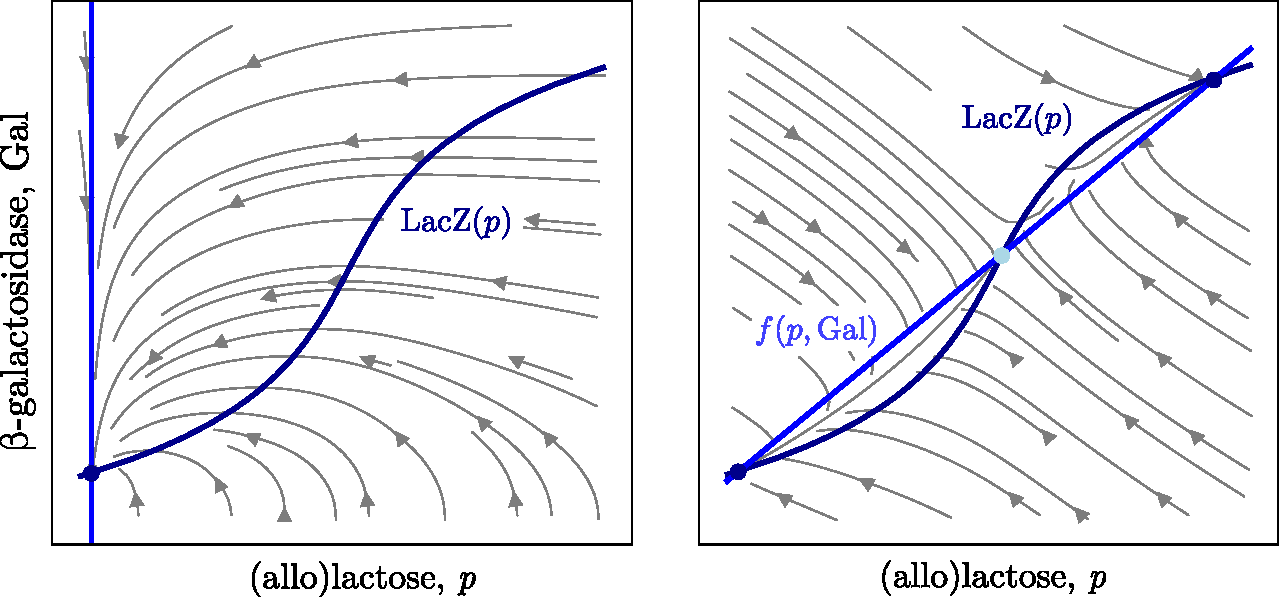
\includegraphics[scale=0.6]{switch}
	\caption{Monostable and bistable behaviour in the lac operon}
	\label{fig:switch}
\end{Figure}

In order to trigger the \emph{switch}-like behaviour we must engineer the dynamics defining the lactose \eqref{eq:lactose-steady} such that it defines a curve intersecting the \emph{hill}-type function three times (Figure \ref{fig:switch}). Mathematically we suppose there exists some $f(p,\mathrm{Gal})$ such that
\begin{align}
	\frac{dp}{dt} = -\beta p\mathrm{Gal} + f(p,\mathrm{Gal})
	\label{eq:lactose-control}
\end{align}
yields three intersections with equation \eqref{eq:gal-steady}. In practice $f$ can come from additional chemical reactions introduced by genetic engineering. We shall see how this was done with non-hydrolysable synthetic analogues of the \emph{lac operon} in Chapter \ref{chapter:double-exclusive}. The main take-away from this analysis is that whenever biochemical reactions yield \emph{hill}-type functions with inflection points, they tend to manifest on steady-state manifolds. This means that with  there is a good chance there exist chemical reactions that use it for its switching behaviour. In fact when the transglycosylation of lactose into \emph{allolactose} is taken into account, bistable behaviour is observed \cite{}.

Now that we've understood how genetic switches can manifest within a single cell, we can begin asking questions about populations of cells. We will do this again in the \emph{mean field approximation}, where a large population of cells can be described as a continuum of spatially extended concentrations $u(x,t)$. Some of molecules can be exchanges between cells, which gives rise to non-zero \emph{diffusion coefficients}, while others are confined within cells. As we shall see in Chapter \ref{chapter:double-exclusive}, a bistable region gives rise to sharp boundaries in gene expression. Such boundaries, their velocity and stability have been studied in the context of \emph{travelling wave solutions} of the \emph{Kolmogorov-Petrovsky-Piskunov equation} \cite{}.

% \subsection{Populations of Neurons \emph{maybe remove}}

\subsection{Self-organised Patterns \& Development}
During the development of any organism a hierarchy of self-organisation takes place that leads to the breaking of symmetry from a spherical cluster of undifferentiated cells to the formation of organ segments and limbs. This process is known as morphogenesis. Figure \ref{fig:morph}, taken from \cite{}, shows an example in which \textit{Hox} gene expression patterns in the body segments of Drosophila can drastically affect its development.

\begin{Figure}
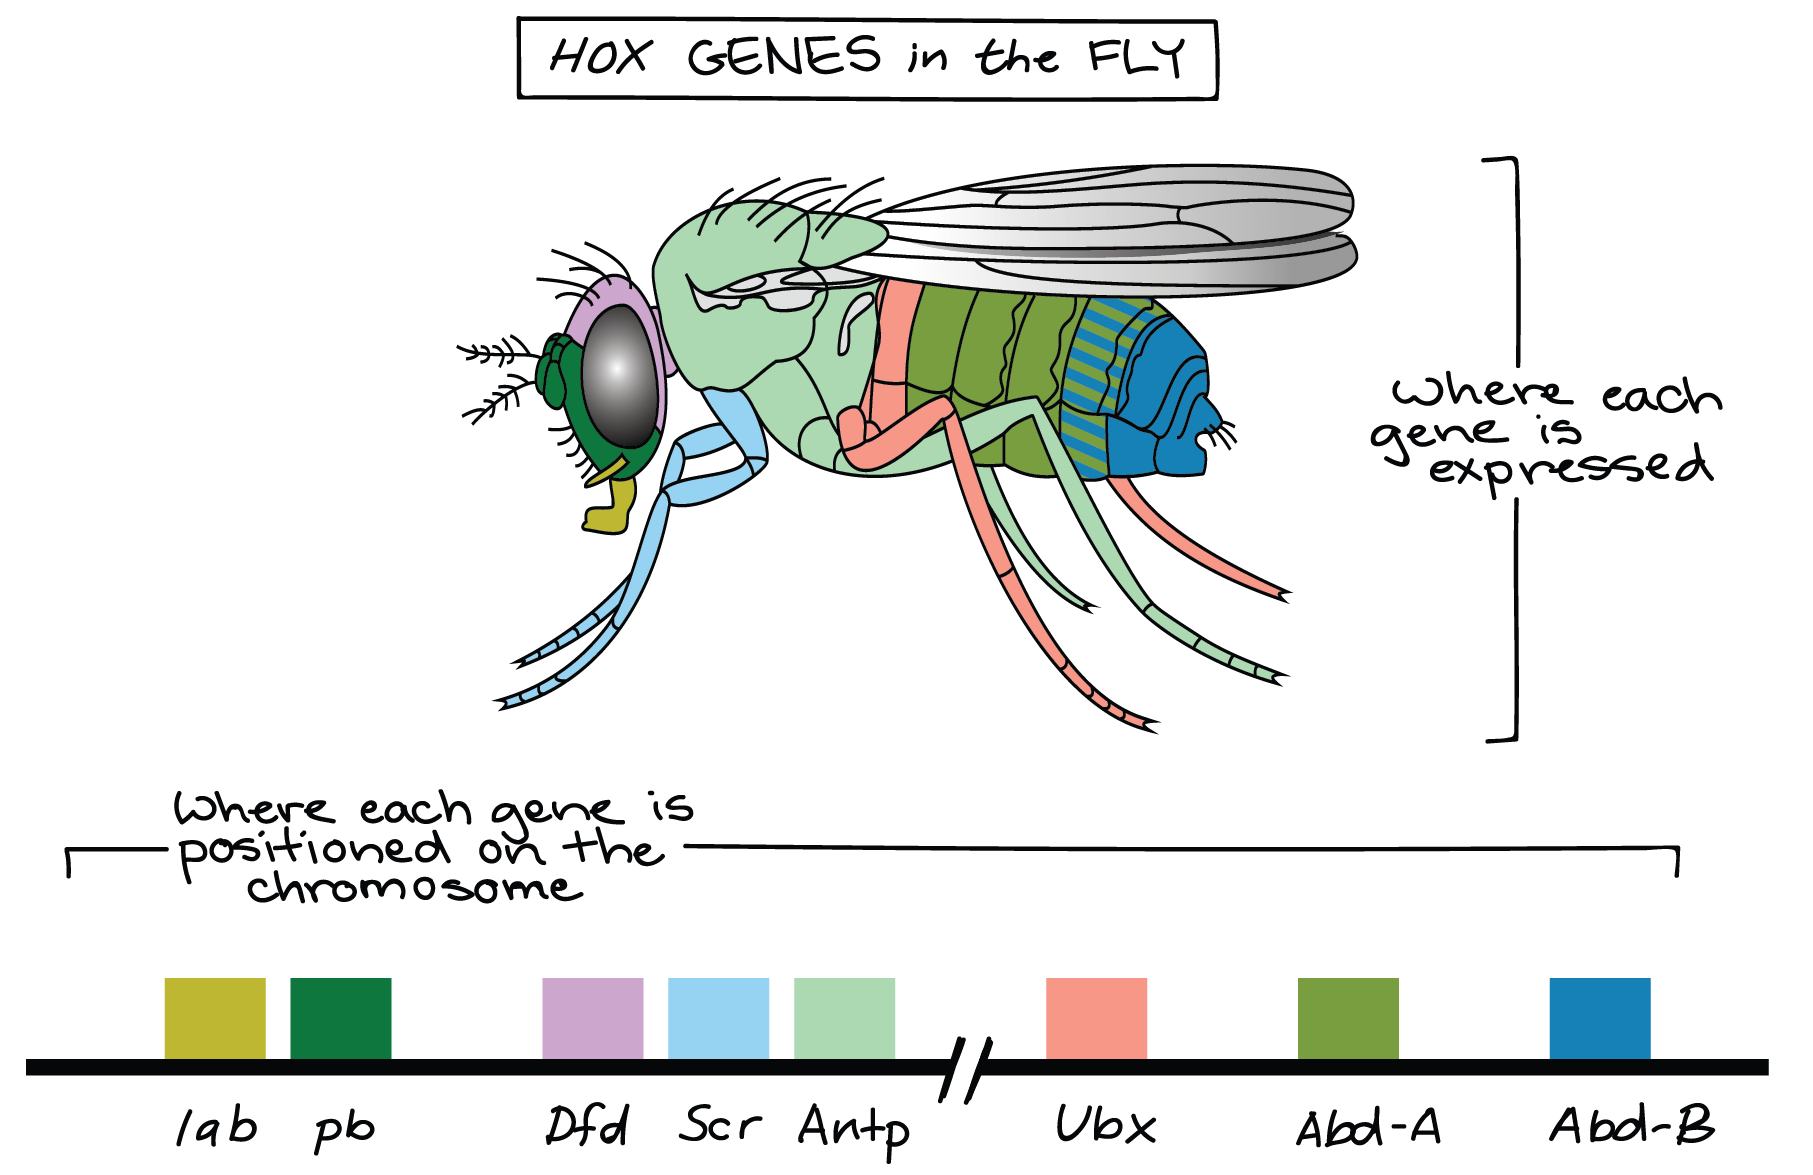
\includegraphics[width=90mm]{figures/morph1.png}\\
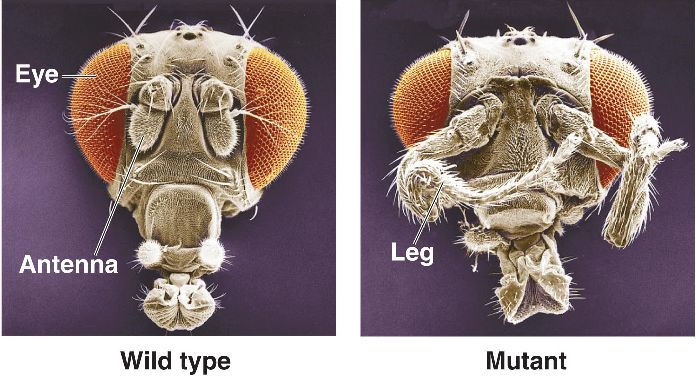
\includegraphics[width=90mm]{figures/morph2.png}
\caption{Top: \textit{Hox} gene expression patterns in body segments of drosophila Bottom: Mutation where legs grow in-place of antenna \cite{}}
\label{fig:morph}
\end{Figure}
\subsubsection{Morphogen-driven Patterns}
One of the central questions in developmental biology is how positional information is sensed by a population of cells and how sharp gene expression boundaries between populations are maintained for robust organ and body segment development. The French Flag model \cite{Wolpert1969PositionalDifferentiation.} proposes that cells have a threshold response to external signalling molecules -- henceforth referred to as morphogens -- which pre-pattern the organism from anterior to posterior and laterally. Some examples of morphogens include Wingless, Decapentaplegic and Sonic Hedgehog. Figure \ref{fig:gap} show the \textit{Gap} expression patterns that partition the Drosophila embryo into segments which are later differentiated by \textit{Hox} genes.

\begin{Figure}
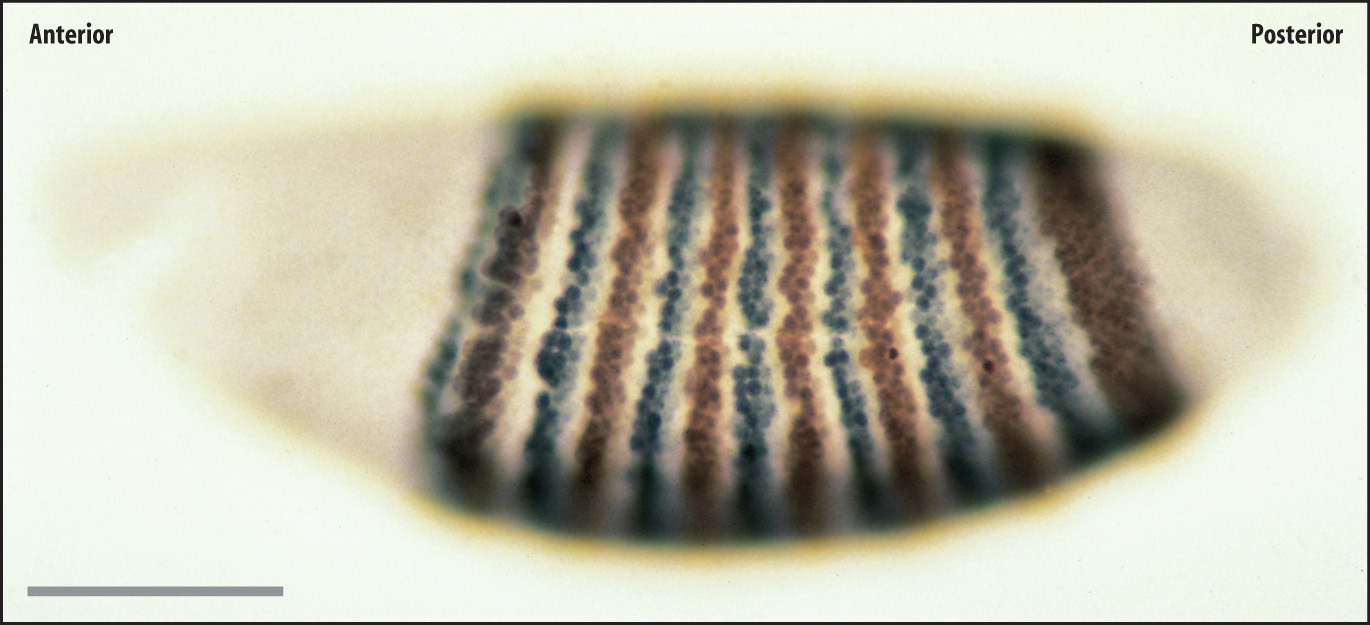
\includegraphics[width=90mm]{figures/gap.jpg}
\caption{Expression patterns of pair-rule \textit{Gap} genes in Drosophila embryo \cite{}}
\label{fig:gap}
\end{Figure}

\subsubsection{Self-organised Patterns}
How are morphogen gradients set up and maintained? How can they be robust against changes in size and geometry? A canonical example of self-organisation in bacteria is the quorum sensing system \cite{Miller2002QuorumBacteria}. Each cell secretes a signalling molecule resulting in the total concentration being proportional to the population density. This signal induces adaptive responses in metabolic and mobility in the whole colony. A long standing mathematical hypothesis that Turing patterns underlie self-organisation in cell populations. Recent literature suggests both morphogen-driven and Turing patterning mechanisms play a role in development \cite{Green2015PositionalCombine}

\begin{Figure}
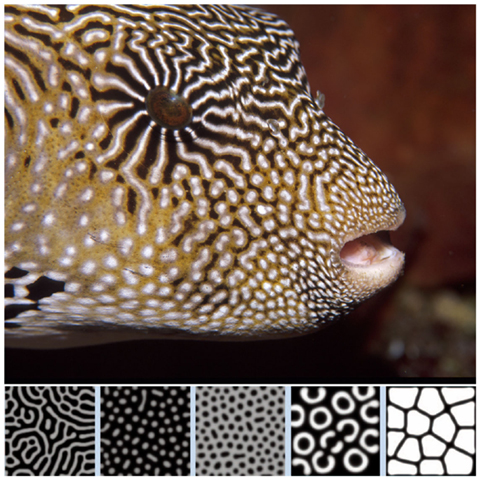
\includegraphics[width=70mm]{figures/turing.png}
\caption{Pigment patterns hypothesised to be generated by Turing mechanism}
\label{fig:turing}
\end{Figure}

\clearpage
\section{Phenotype Inference with Machine Learning}
\label{section:phenotype-inference}

Thus far we have outlined how applying bifurcation analysis to a model $\rates(u,p)$ relating the organism state $u$ to environmental conditions $p$ and genotype $\theta$ can be used to distinguish its phenotypes. What do we do in circumstances where the model is partially or completely unknown? In this case, rather than deriving the functional forms relating states $u$ from reasonable biochemical assumptions and mass-action laws, we rely on \emph{universal function approximators} \cite{}.
\begin{Figure}
    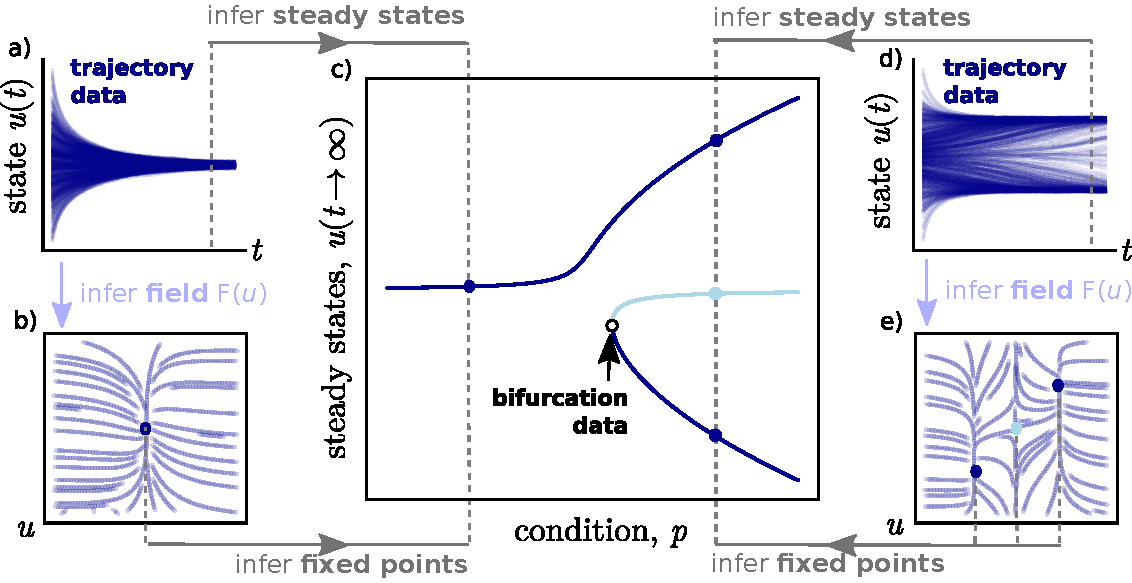
\includegraphics[width=14cm]{inferring-bifurcations}
    \caption{Bifurcation point extraction along the condition $p$ via two possible routes: steady state inference (a,d$\rightarrow$c) and fixed point inference (a,d$\rightarrow$b,e$\rightarrow$c). The fixed point inference route requires \emph{universal function approximator} $F(u)$ at different values of the condition $p$ and yields additional unstable fixed points.}
    \label{fig:inferring-bifurcations}
\end{Figure}
When a model $\rates(u,p)$ is absent it becomes difficult to know which observations to collect. In the era of high-throughput biology, the solution to this is to simply collect as many observations as possible and search the high-dimensional data for mechanisms that elucidate what the organism model could be. Such data may include flow cytometry, proteomics (MS/MS), transcriptomics (scRNA-seq) metabolomics (MS) and a wide variety of next-generation sequencing data \cite{}. Thus the problem of differentiating phenotypes becomes a matter of extracting bifurcations from high dimensional \emph{universal function approximators}.

Bifurcations along conditions $p$ can be extracted from data via two possible routes as depicted in Figure \ref{fig:inferring-bifurcations}: via a \emph{universal function approximator} $F(u)$ which enables the location of all fixed points, including unstable ones, or via direct inference from steady state data $u(t\rightarrow\infty)$. At best we could have state trajectory data $u(t)$ like single cell trajectories extracted via segmentation and tracking in fluorescence microscopy movies (for example the data acquired using the CellASIC ONIX Microfluidic Platform in Figure \ref{fig:double-exclusive:bistability}c). The majority of biomedical data is sparsely sampled with respect to time (for example the flow cytometry measurements in Figure \ref{fig:double-exclusive:flow-hysteresis} which were only collected at experiment end-points) and in such settings expecting to capture dynamical transients which would reveal the locations of unstable fixed points would be unreasonable. If we assume that the data was collected at a time where the organism is in homeostasis, then we can infer the steady states $u(t\rightarrow\infty)$ and any possible bifurcations directly from statistical measures of the data without needing a \emph{universal function approximator} $F(u)$. The emergent picture suggests a model of the state space $F(u)$ is desirable because it fully characterises the phenotype, but requires data or prior knowledge about dynamical transients of the organism. Fortunately, as we will see, statistics on the organism in homeostasis reveal stable steady states and static bifurcations.

\clearpage
\subsection{Phenotypes from Statistics in Homeostasis}
\label{section:steady-state-inference}
Suppose we collected an $N$-dimensional $K$ cell omics dataset $\mathbf{U}\in\Reals^{N\times K}$ from an organism of genotype $\theta$ in various conditions $p$. We would like to know how many cell phenotypes there are in our dataset and how they may change in response to changes in environment $p$ or genetic manipulation $\theta$. Formally the dataset is an $N\times K$ matrix with $K$ samples $U\in\Reals^N$ along columns. We suppose there exists a steady state probability density $P_{\theta}(u,p)$ for a particular genotype $\theta$ and condition $p$ from which the samples $U$ are generated from.
\begin{equation}
	\mathbf{U} := \begin{pmatrix}
		\mid&\mid &        & \mid\\
		U_1 & U_2 & \cdots & U_K\\
		\mid&\mid &        & \mid
	\end{pmatrix}
	\where 
	U \sim P_{\theta}(u,p)
\end{equation}
Dimensionality reduction in tandem with 
Suppose we would like to detect a cusp bifurcation and limit points in a cell population with respect to two experimental control conditions $p,p\prime\in\Reals$. We can set up a serial dilution along the columns for $p$ and along the rows for $p\prime$ in two 96-well plates. Cells allowed to grow in exponential phase in a finite concentration of either $p\ll p\prime$ or $p\gg p\prime$. Let us call this the \emph{priming} stage of the protocol as shown in Figure \ref{fig:cusp-sampling}a, resulting in two cell populations: $p$-primed cells and $p\prime$-primed cells. The priming concentrations must be chosen sufficiently high so that the resultant population states lie either side of the cusp. The two populations are transferred into separate 96-well plates containing the dilutions of $p,p'$; we call this the \emph{conditioning} stage in Figure \ref{fig:cusp-sampling}a.

\begin{Figure}
    \includegraphics[width=14cm]{hysteresis}
    \caption{Protocols (a) for extracting limit points with respect to conditions $p,p'$. Steady state distributions (b). Similarity measure (c)}
    \label{fig:cusp-sampling}
\end{Figure}

The cells are then transferred into a flow cytometer, gated for live singlets and processed with relevant compensation and auto-fluorescent normalisation, which would produce the population distributions $P(u)$ for the $p$-primed cells and $Q(u)$ for $p'$-primed cells in each well. By overlaying distributions $P(u),Q(u)$ for each well, a figure similar to Figure \ref{fig:cusp-sampling}b (or Figure \ref{fig:double-exclusive:flow-hysteresis}) can be produced. Finally, the limit points can be defined by a level set of distribution similarity measure $D(P||Q)$ in the $p,p\prime$-plane as shown in Figure \ref{fig:cusp-sampling}c. This similarity measure could be Kullback–Leibler divergence or something as simple as the distance between distribution medians. The level set must be some small positive amount $\epsilon$ above zero, picking out the onset of dissimilarity between steady state distributions $P(u)$ and $Q(u)$, and hence the onset hysteresis. We can define the limit points as
\begin{align}
    \targets = \{  (p,p\prime) : D(P||Q)=\epsilon, \epsilon>0 \} 
\end{align}

This approach may break down if multi-modal distributions exist in the data. This would be the case if something happened to prevent a subpopulation of cells to switch from one state another other. Reasons for this could include too much cell burdon or not enough time given for cells to reach a steady state. In this case, quantifying the efficiency of switching from either side of the cusp could be a quantity of interest.

This approach would not work for extracting dynamic bifurcations such as \emph{Hopf} since only steady state information is available. Furthermore, the accuracy of this method is subject to noise amplitude. This method works well for cases where changes in the number of stable steady states can be resolved in the measured steady state distributions.

\begin{itemize}
    \item quantify efficiency of switching?
\end{itemize}

Having the the state as a function of time $u(t)$, sampled at sufficiently broad initial conditions $u(0)$, enables the estimation of field geometry $F(u)$ via \emph{universal function approximators} such as neural networks \cite{Chen2018NeuralEquations} and Gaussian processes \cite{Seeger2004GaussianLearning.}. We refer the reader to a modern review of the most successful machine learning approaches for designing \emph{universal function approximators} \cite{Bronstein2021GeometricGauges} where emphasis is made on understanding how group equivariant and group invariant transformations are stacked together. Note that we've dropped $\theta$ and $p$ from the \emph{universal function approximator}. We reserve $\theta$ to be a vector of biophysically meaningful parameters that make up an organism genotype. While \emph{universal function approximators} typically have a lot of parameters, they tend not to reveal the mechanism under study and hence cannot be used to deduce which genetic design interventions can be made.

% We can then extract important state-space structures, such as stable and unstable fixed points, their eigenvalues $\lambda$, from the field geometry $F(u)$ at different values of the control condition $p$, and hence identify possible bifurcations.


% Data on steady states $u(t\rightarrow\infty)$ are more abundant and typically found in flow cytometry measurements. It is possible to infer the steady state manifold directly from such data (Figure \ref{fig:inferring-bifurcations} a,d$\rightarrow$c) but we would not be able to extract information on unstable fixed points or eigenvalues $\lambda$ of state-space structures. Since the criteria for bifurcations are not directly accessible, indirect measures (such as the population separation that can be seen in Figure \ref{fig:double-exclusive:flow-hysteresis}) must be used to extract bifurcations.


% \subsection{Classification and Regression}
% \begin{itemize}
%     \item Logistic regression
%     \item Nearest neighbour methods
%     \item Mixture Models
% \end{itemize}

% \subsection{Dimensionality Reduction Methods}
% \begin{itemize}
%     \item UMAP and Tsne
%     \item Sloppy parameters and identify-ability
% \end{itemize}

% \subsection{Clustering Methods}

\section{Applications in Flow Cytometry}
\label{section:applications-flow-cytometry}


\subsection{Immunophenotyping Panels}



\subsubsection{Non-parameteric Vector Field Inference}
% Non-parametric ___ using Gaussian Process regression
\label{section:field-inference}

In this early days of this thesis, we investigated whether it was possible to transform the time-domain data into state-space. This approach, and related works, are discussed in this section and can in principle be used with the microfluidic fluorescence microscopy data for parameter inference.

Consider we are given $K$ cell trajectories $\mathcal{D}_1$, $\mathcal{D}_2$ ... $\mathcal{D}_K$, each containing $N$ noisy observations of the state of the cell. Let the cell state be represented by state vector $u(t)\in\Reals^N$ which is hypothesized to obey a set of ordinary differential equations of the form \eqref{eq:differential-equations}. Instead of integrating the equations \eqref{eq:differential-equations} we would find an estimate for the derivative of the trajectories $\hat{f}$.

This is known as the \textit{smoothing} step \cite{Gugushvili2012Smoothing} should be done using unsupervised methods, for example with Gaussian Process Regressors \cite{Seeger2004GaussianLearning.} as shown in in Figure \ref{fig:inferred-cycles}. This requires the inversion of an $K'\times K'$ data matrix where $K':=\sum_k |\mathcal{D}_k|$ is the total number of trajectory data points. This has a computational complexity $K'^3$ which is only tractable with sparse datasets.

Let the region $\partial\mathcal{D}$ be a boundary defined by the Delaunay tessellation of the input data. Let us define the estimate $\hat f$ only within the region $\partial\mathcal{D}$ so that there are no extrapolation artefacts. For the Gaussian Process approach the estimate would be
\begin{equation}
    \hat{f}(u)\sim
        \mathcal{N}(\,\mu(u) ,\Matrix{\Sigma}(u)\,)
    \quad\mathrm{for}\quad u\in\partial\mathcal{D}
\end{equation}
\noindent where at any given state $u$ the field estimate $\hat{f}$ is generated by Gaussian distributions of mean vector $\mu$ and covariance matrix $\Matrix{\Sigma}$.Solving for these requires a choice of matrix-valued kernel function $\Matrix{K}(u,v)$ which encodes our knowledge about the local structure of the field. Sophisticated kernels for learning vector fields exist \cite{Fuselier2017ADecompositions} for decomposing fields in conservative and solenoidal components, which aid in localising fixed points and cycles.

The simplest choice of kernel assumes the components are independent and have a finite correlation length $\gamma$, such as Gaussian radial basis functions. Here $\Matrix{I}$ is the identity matrix and the hyperparameter $\gamma$ has to be optimised.
\begin{equation}
    \Matrix{K}(\Vector{u},\Vector{v}) = \Matrix{I}\,\mathbb{e}^{-\gamma|\Vector{u}-\Vector{v}|^2}
\end{equation}

The second step is called \textit{matching} where the estimated field $\hat{f}$ is used as an optimisation target against some parametrised function $\rates$ with unknown parameters $\theta$.

In our setting we would like to match the geometry of the field but not its magnitude; in this sense we are focusing on the qualitative aspects of the dynamics of a set of differential equations, rather than the quantitative dynamics or kinetics. This could be achieved with the following objective function
\begin{equation}
    \mathcal{L}(\theta|\mathcal{D}) := \e^{-\frac{\hat{f}\cdot\rates}
    {|\hat{f}||\rates|}}
\end{equation}
\noindent where the cost is minimal when the data derivative $\hat{f}$ and the parametrised model $\rates$ point in the same direction and maximal when they point in opposing directions.

\begin{Figure}
    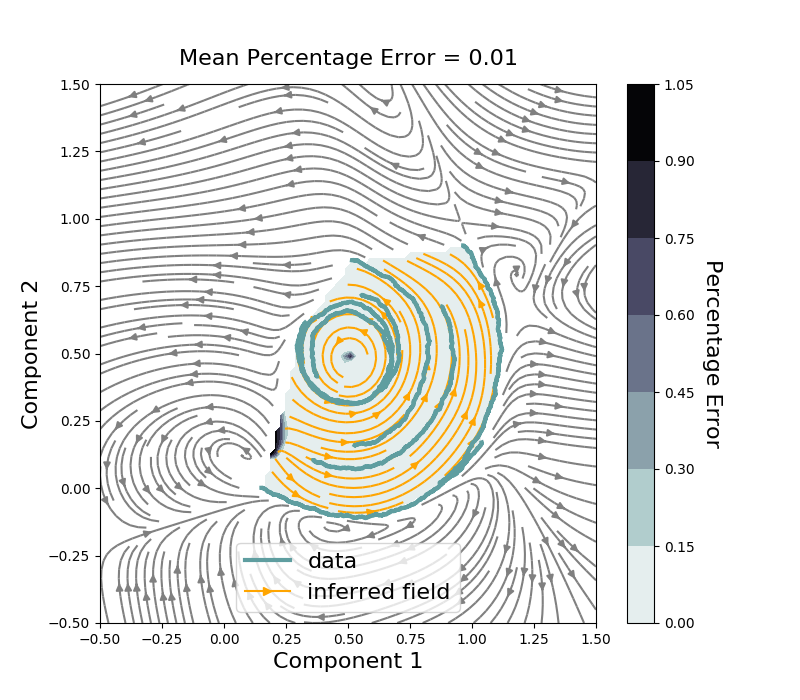
\includegraphics[width=125mm]{figures/cycle-2.png}
    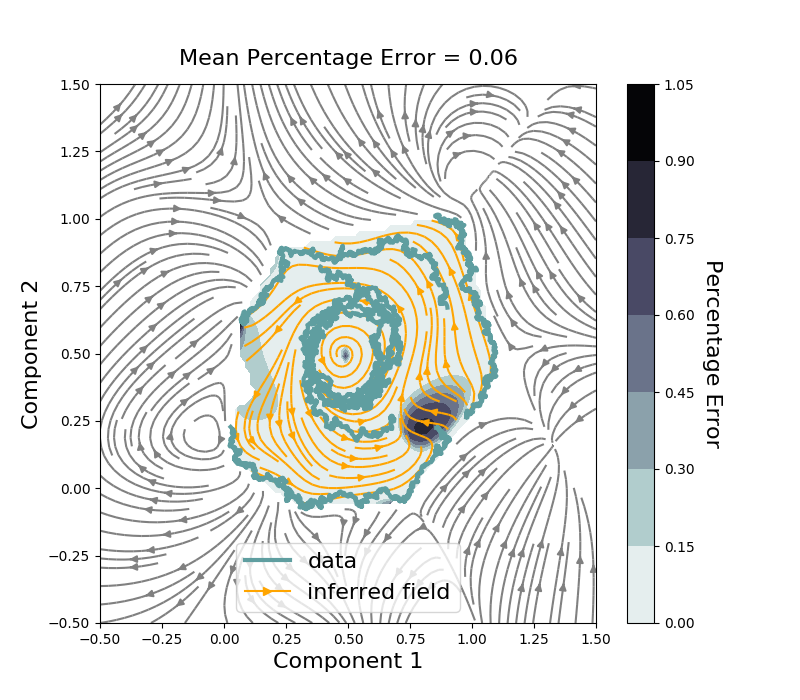
\includegraphics[width=125mm]{figures/cycle-1.png}
    \caption{Gaussian process regressors estimating derivative of the trajectories $\hat{f}$ from example trajectory datasets $\mathcal{D}_1$ ... $\mathcal{D}_K$ with varying signal to noise ratios. Interpolation error $E$ is shown as a heatmap; extrapolation fails}
    \label{fig:inferred-cycles}
\end{Figure}

Although we are getting close to focusing on qualitative features of a model, this objective function is still sensitive to the locations and shapes of fixed point and limit cycles. What if we cared about even higher-level features such as the number of fixed points? Or perhaps whether a system oscillates or not? This is where the language of bifurcation theory described in Chapter \ref{chapter:background} is optimally suited for this task, but fist we need to discuss how to set up experiments to detect bifurcations from flow cytometry data.

\begin{itemize}
    \item Vector field estimates too noisy to get bifurcation points?
    \item Divergence and the stability of fixed points
    \item curl and limit cycles. How does this relate to hopf example \ref{fig:inferred-cycles}
    \item Do we need a bistable example?
\end{itemize}

The accuracy of the cell trajectories is limited by cell segmentation and tracking algorithms. Initial investigations into this approach also suggested that trajectories need to be of sufficient temporal resolution and sampled from a wide variety of initial conditions. Such data is not widely available and ultimately we decided to focus on a method that could be used with a well-known workhorse in biomedical research: flow cytometry.

\subsubsection{Fixed Point Inference}
\label{section:fixed-point-inference}
\chapter{Interpretation of Morphogen Gradients by a Bistable Circuit}
\label{chapter:double-exclusive}
\epigraph{\textit{memory of younger days}}{Ocarina of Time}
\section{Preface}
\subsection{Problem Statement \& Context}

\begin{enumerate}
    \item Keep focus on developmental biology
    \item Revised supplement as this chapter
\end{enumerate}

\usetikzlibrary{patterns}
\begin{Figure}
\begin{tikzpicture}
\def\H{3.5}
\def\L{10.0}
\def\l{1.0}
\def\epsilon{0.5}
\def\dx{0.25}
\def\dy{0.25}

%cell region
\filldraw[fill=Red!50!white] (\l,\H) rectangle (\L-\l,\H+\epsilon) node[midway] {Cells};

%agar region
\filldraw[fill=Dandelion!10!white,draw=black] (0,0) rectangle (\L,\H) node[midway] {Agar};
\fill[pattern=north east lines, pattern color=cyan] (0,0) rectangle (\l,\H) node[midway] {\begin{tabular}{c}Agar\\+\\$C_6$\end{tabular}};
\fill[pattern=north east lines, pattern color=yellow!80!black] (\L-\l,0) rectangle (\L,\H) node[midway] {\begin{tabular}{c}Agar\\+\\$C_{12}$\end{tabular}};
\draw[|<->|](0,-\dy) -- (\L,-\dy) node[midway, below] {$L$} ;
\draw[|<->|](0,\dy) -- (\l,\dy) node[midway, above] {$l$} ;
\draw[|<->|](\L-\l,\dy) -- (\L,\dy) node[midway, above] {$l$} ;
%\draw[|<->|](\L+\dx,0) -- (\L+\dx,\H) node[midway, right] {$H$} ;
%\draw[|<->|](\L+\dx,\H) -- (\L+\dx,\H+\epsilon) node[midway, right] {$H_\varepsilon$} ;

%axis
%\draw[->] (-\dx-\dy,-\dy)--(0.1*\L,-\dy) node[right] {$x$};
%\draw[->] (-\dx,-\dx-\dy)--(-\dx,0.5*\H) node[above] {$y$};
\end{tikzpicture}
\caption{Geometry of opposing gradients experiment}
\label{fig:experiment_geometry}
\end{Figure}

This section outlines how the Design---Learn pipeline may help achieve a specific
aim in a typical collaboration between theory, computation and experiment.
The aim of this project is to reconstitute and control minimal self-organisation
mechanisms which are believed play crucial roles in developmental biology. To this
end \textit{E. Coli} has been genetically engineered to produce orthogonal responses
to two different input signals --- henceforth this organism will be referred to as the
\textit{double exclusive reporter} circuit \cite{Grant2016}. The colony of reporters
serve as a reduced model for a multi-cellular organism during embryonic stages of
development. While patterns with sharp boundaries have successfully been realised,
producing Turing instabilities remains challenging as the system needs to be such
that patterns develop before the colony reaches stationary phase.
The role of theory and computation in this project is to help identify the
parameter regimes that produce controllable and self-organised patterns.

\subsection{Contributions}

\textbf{Grisha Szep} is co-second author with \textbf{Om Patange} (University of Cambridge, UK). \textbf{Paul Grant}, \textbf{Neil Dalchau}, \textbf{Jacob Halatek} and \textbf{Andrew Phillips} (all Microsoft Research Cambridge, UK) conceived and designed the study. \textbf{Paul Grant} designed and built the genetic circuits. \textbf{Paul Grant}, \textbf{Om Patange} and \textbf{Valerie Coppard} (Microsoft Research Cambridge, UK) performed the experiments. \textbf{Grisha Szep}, \textbf{Jacob Halatek} and \textbf{Neil Dalchau} conceived and implemented theory and modelling and wrote the supplementary information. All authors analysed and interpreted the data. \textbf{Paul Grant} and \textbf{Andrew Philips} wrote the main text. All authors provided input into the manuscript. The contributions of \textbf{Grisha Szep} the main text and supplementary include:
\begin{itemize}
    \item \textbf{Figure 1.b} Spatial simulations of parameterized model
    \item \textbf{Figure 2.a-b} Calculation of region of bistability predicted by the parameterized model using arc-length continuation algorithms
    \item \textbf{Figure 3.b-e} Wrote bespoke inference code for quantification of boundary velocity from microscopy movies and comparison to theoretical model
    \item \textbf{Figure 4.d-e} Spatial simulations of the parametrized model. Novel state-space analysis of boundary formation and bistability
    \item \textbf{Figure S10.c} Spatial simulations analysed in state-space
    \item \textbf{Figure S13} A novel method for quantifying hysteresis in the flow cytometry experiments as population separation
    \item \textbf{Figure S25-S26} Bistability analysis of parametrized models and comparison to qualifications from flow cytometry
    \item \textbf{Figure S27-S33} Simulations of boundary velocity, novel way of understanding them in state space and bespoke inference methods for quantification of boundary velocity from microscopy movies
    \item \textbf{Figure S36} State space geometry for model with feedback loops
    \item \textbf{Supplementary Sections 2.2-2.4} Wrote sections outlining the methods for extracting bistability regions from data and models with and without feedback loops
    \item \textbf{Movies 1-5} Simulations of expression boundary formation
    \item \textbf{Code} Released code with documentation in \href{https://github.com/gszep/double-exclusive-reporter}{GitHub Repository}
\end{itemize}

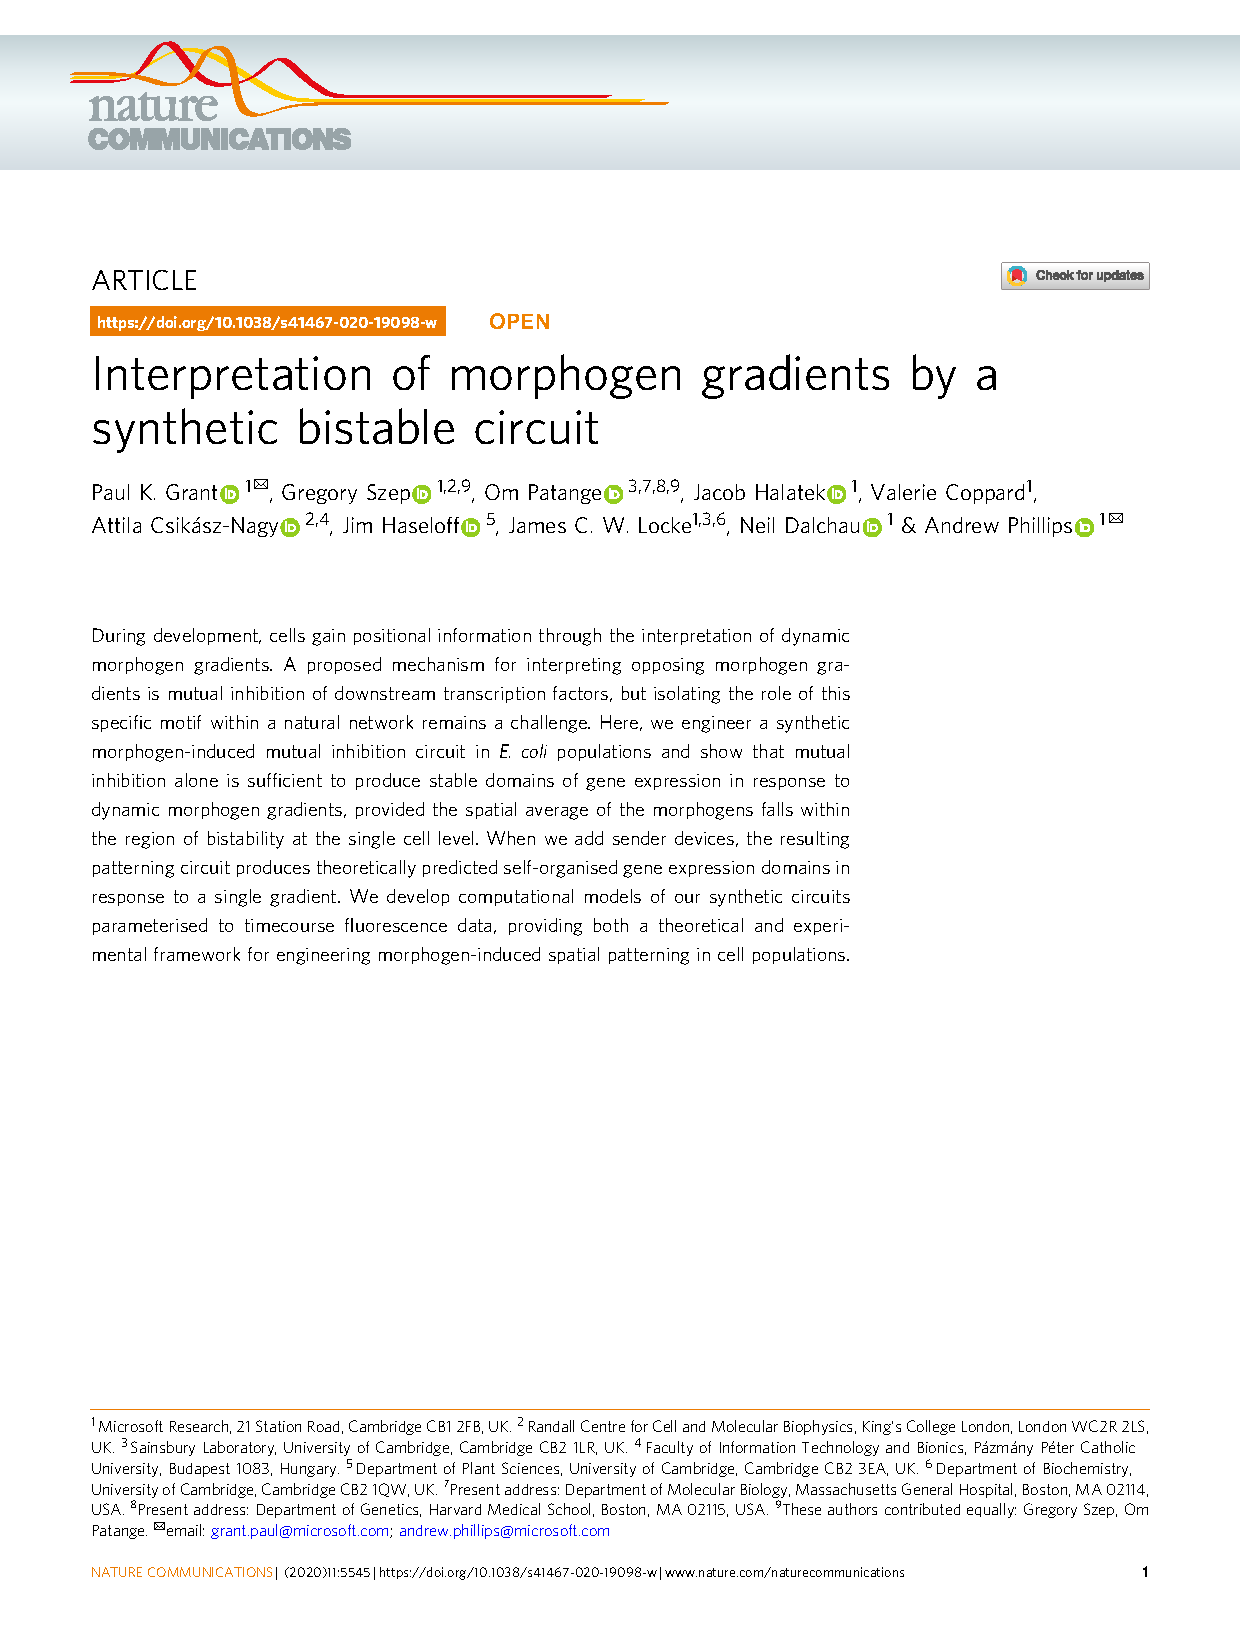
\includepdf[pages=1-8, offset=75 -90, scale=0.85, frame,
        clip,trim=10mm 5mm 10mm 0mm,
        pagecommand={}, addtotoc={
        1,section,1,Abstract,double-exclusive:abstract,
        2,section,1,Introduction,double-exclusive:introduction,
        2,section,1,Results,double-exclusive:results,
        2,subsection,2,Engineering mutual exclusivity,double-exclusive:exclusivity,
        3,subsection,2,Mutual inhibition results in bistability,double-exclusive:bistability,
        4,subsection,2,Hysteresis produces stable boundaries,double-exclusive:boundaries,
        4,subsection,2,A secondary gradient creates self-organised domains,double-exclusive:self-organisation,
        5,section,1,Discussion,double-exclusive:discussion,
        6,section,1,Methods,double-exclusive:methods,
        6,subsection,2,Plasmid construction,double-exclusive:plasmids,
        6,subsection,2,Plate fluorometer assay,double-exclusive:plates,
        6,subsection,2,Flow-cytometric analysis of hysteresis,double-exclusive:flow,
        7,subsection,2,Microfluidics,double-exclusive:microfluidics,
        7,subsection,2,Microfluidics microscopy,double-exclusive:microscopy,
        7,subsection,2,Solid culture assays,double-exclusive:cultures},
    addtolist={
        2, figure, {\textit{Fig. 1}\quad A synthetic gene circuit for morphogen interpretation.}, fig:double-exclusive:overview,
        3, figure, {\textit{Fig. 2}\quad Mutual inhibition produces bistability.}, fig:double-exclusive:bistability,
        5, figure, {\textit{Fig. 3}\quad Formation of stable boundaries.}, fig:double-exclusive:boundaries,
        6, figure, {\textit{Fig. 4}\quad Addition of a Relay circuit creates self-organised domains of gene expression.}, fig:double-exclusive:relay
}]{publications/double-exclusive.pdf}

\section{Afterword}

The decision to focus on single cell trajectories and flow cytometry came from the limitations of using microplate data in Chapter \ref{chapter:double-exclusive}. The model parameters $\theta$ were estimated using a hierarchical monte-carlo approach and time-course fluorescence microplate measurements (details of which can be found in Appendix \ref{appendix:double-exclusive:inference}). The time-courses include information about dynamical transients and colony growth in liquid culture. The desired cusp bifurcation, however, lives in state-space rather than the time-domain. The disconnect between the domain that the data lives in and the domain of the design goals poses the risk of over-fitting the model on undesired information that exists in the data domain. 

It is not possible to observe the cusp bifurcation in microplate data, due to the averaging of signals originating from heterogeneous cell populations. Instead, the cusp bifurcation can be observed in flow cytometry measurements of colonies in exponential phase (Supplementary Figure \ref{fig:double-exclusive:flow-hysteresis}) and microfluidic fluorescence microscopy data (Figure \ref{fig:double-exclusive:bistability}c) where computations on single-cell trajectories reveal the hysteresis loop which must necessarily accompany the cusp. 
\chapter{Parameter Inference with Bifurcation Diagrams}
\label{chapter:inference}
\begin{music}
    \parindent10mm \instrumentnumber{1} \setstaffs1{1} 
    \generalmeter{\meterfrac44} \generalsignature{2}
    \startextract
            \notes \ql j \ql i \Qqbl ieji \en
        \bar \zw{m*} \bar 
            \notes \ql i \qu h \Qqbu hdih \en
        \bar \zw{l*} 
    \zendextract
\end{music}
\epigraph{\textit{the melody that will draw you into the infinite darkness}}{Nocturne of Shadow --- Ocarina of Time}

\section{Preface}
\subsection{Problem Statement \& Context}
This chapter focuses on the problem of looking for parameter regimes for dynamical systems that result in bifurcations. This has been coined as \emph{inverse bifurcation analysis} \cite{Lu2006InverseSystems}. Formally we are looking for parameters $\theta$ for which the equation \eqref{eq:differential-equations} has at least one fixed point for which bifurcation criteria (see Section \ref{section:bifurcation-analysis}) are satisfied. These bifurcations are to be placed along control condition $p\in\Reals$.

Inverse bifurcation analysis becomes relevant to biomedical researchers in settings where there is a design goal to engineer an organism with a distinct phenotype (as discussed in Chapter \ref{chapter:introduction}).
In Chapter \ref{chapter:double-exclusive}, we introduced the \emph{double exclusive reporter}, which was engineered in \emph{E. Coli}, and exhibits a cusp bifurcation leading to a bistable response with respect to two input signals (Figure \ref{fig:double-exclusive:bistability}). The engineering goal could be a phenotype with a specific cell cycle \cite{Attila2008,Conrad2006BifurcationClock} which involves the positioning of \emph{Hopf bifurcations} that mark the onset of oscillations in protein concentrations from stable equilibria. Finally the design of self-organised patterns such as stripes and spots in mammalian coat patterns could be another engineering goal. Controlling the mechanisms that underpin morphogenesis and development may involve the search for \emph{Turing bifurcations} \cite{Turing1952}.

Before we get carried away and think that with the right tooling we could genetically control the length scale of spots or stripes on cats, we must remind ourselves that \emph{in vivo} gene regulatory networks mostly consist of unknown and experimentally inaccessible parameters. Furthermore, we find that usually there exist multiple equally valid models that describe the observed behaviour, and so turn to \emph{model selection} methods. Even if we had an accurate and unique model to describe an organism, generic tools for \emph{inverse bifurcation analysis} are limited as we've explored in Chapter \ref{chapter:background} and experienced in practice in Chapter \ref{chapter:double-exclusive}. In an attempt to address these limitations, the incorporated publication (sections \ref{inference:abstract} -- \ref{inference:impact}) and supplementary material (Appendix \ref{appendix:inference}) published in \textit{Advances in Neural Information Processing Systems 35} focuses on the design of systems of ordinary differential equations with \emph{pitchfork} and \emph{saddle-node} bifurcation diagrams. Although the publication focuses on parameter synthesis for a subset of bifurcations, steps towards \emph{Hopf} bifurcations are made (see Appendix \ref{appendix:hopf-measure}), and the approach lays foundations for differentiable optimisation methods that leverage bifurcation theory. A view towards how this approach can be used for the design of \emph{Turing patterns} and model selection is discussed in concluding Chapter \ref{chapter:conclusions}.
\subsection{Contributions}
\textbf{Grisha Szep} prepared the manuscript, designed the cost function, derived mathematical results, wrote and released the Julia package under the supervision of \textbf{Neil Dalchau} and \textbf{Attila Csikasz-Nagy}.

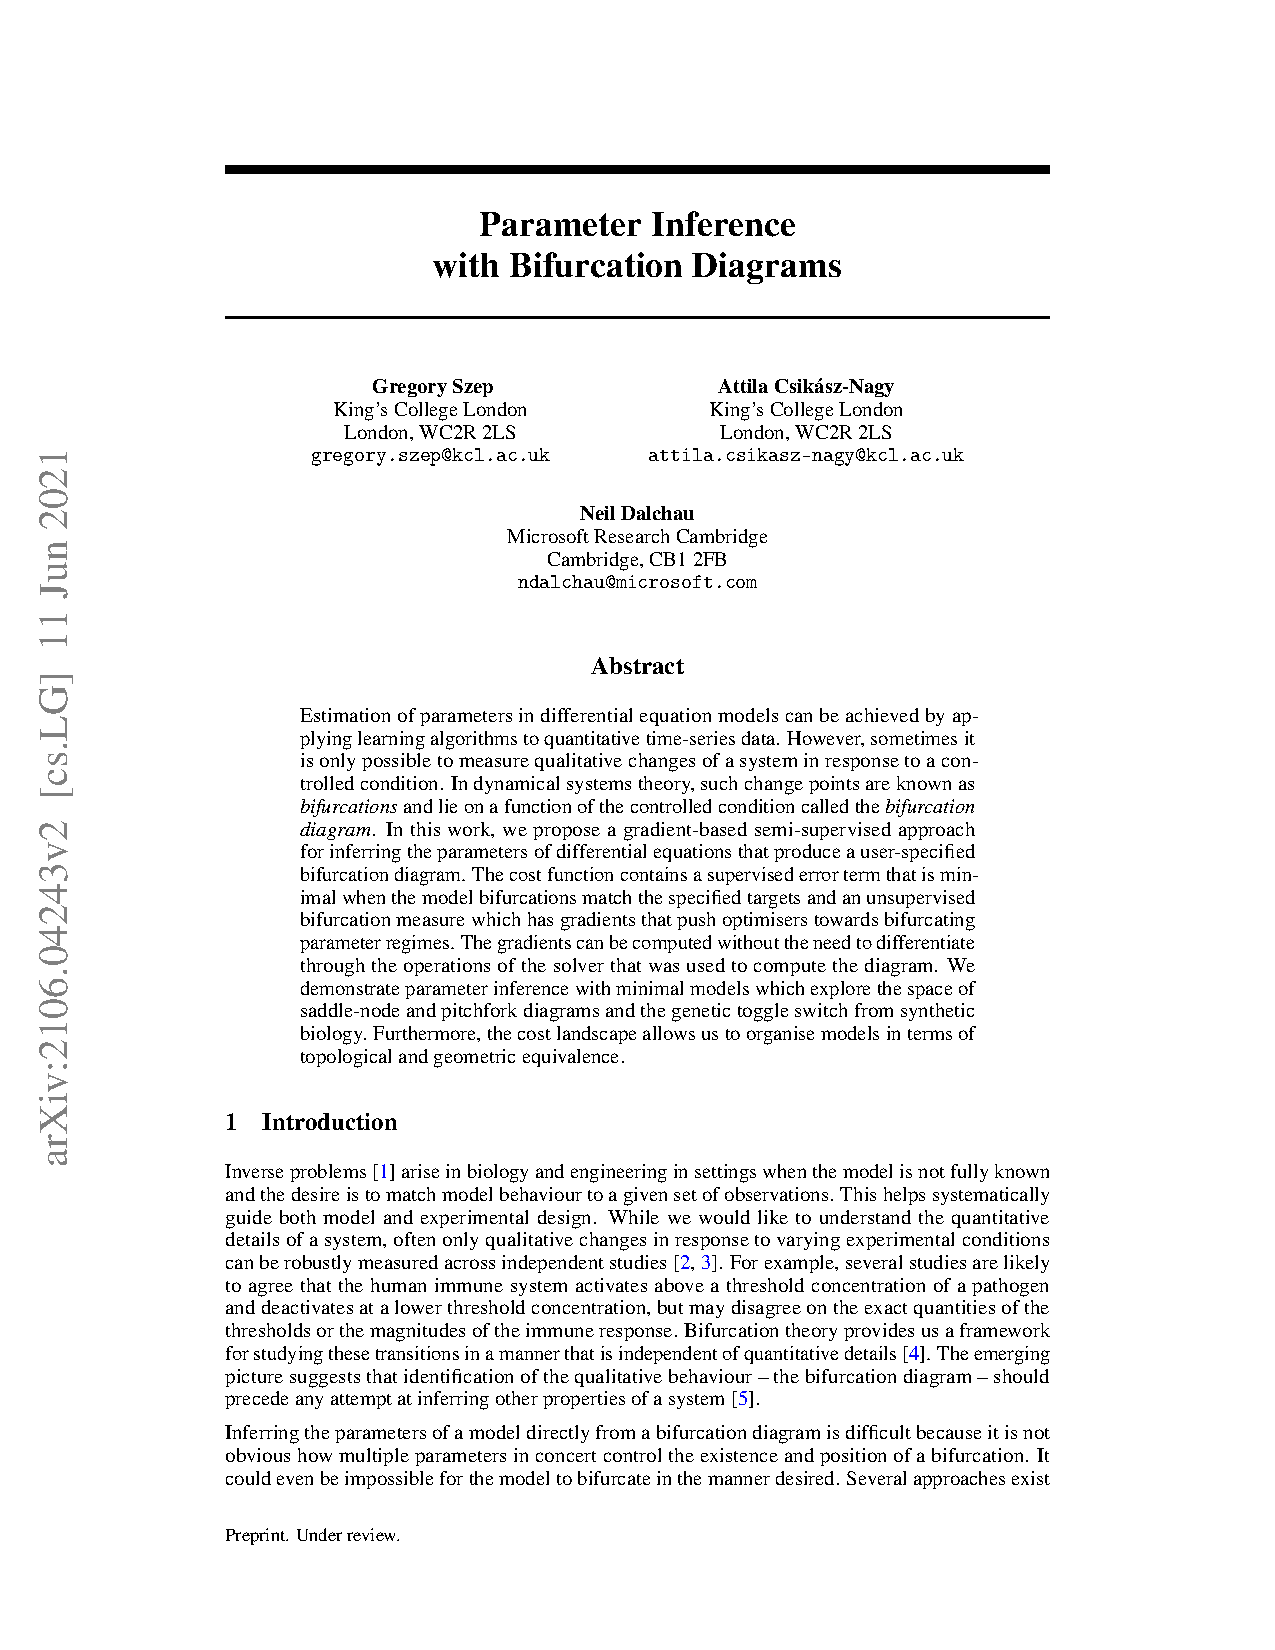
\includepdf[pages=1-11, offset=75 -95, scale=0.85, frame,
        clip,trim=31mm 21mm 31mm 21mm,
        pagecommand={}, addtotoc={
        1,section,1,Abstract,inference:abstract,
        1,section,1,Introduction,inference:introduction,
        2,subsection,2,Preliminaries,inference:preliminaries,
        4,section,1,Proposed Method,inference:method,
        4,subsection,2,Semi-supervised Cost Function,inference:cost,
        5,subsection,2,Differentiating the semi-supervised cost function,inference:derivatives,
        6,section,1,Experiments \& Results,inference:results,
        6,subsection,2,Minimal Models,inference:minimal,
        6,subsection,2,Genetic Toggle Switch,inference:genetic,
        7,subsection,2,Complexity,inference:complexity,
        9,section,1,Conclusion \& Broader Impact,inference:impact},
    addtolist={
        3, figure, {\textit{Fig. 1}\quad Illustration of bifurcation diagrams for minimal models of bifurcations. A. Saddle-node bifurcations arise for $\rates(u,p) = p + \theta_{1}u+\theta_{2}u^3$ when $\theta = (\frac{5}{2},-1)$. B. Pitchfork bifurcations arise for $\rates(u,p) = \theta_{1} + p u+\theta_{2}u^3$ when $\theta=(\frac{1}{2},-1)$. Targets are illustrated by light yellow vertical lines. Bifurcation curves are shown as solid blue and red lines, with lighter shades indicating the determinant crossing zero at locations $\predictions(\theta)$ giving rise to unstable solutions.}, fig:inference:minimal-models,
        4, figure, {\textit{Fig. 2}\quad Bifurcation measure $\measure(s)$ and determinant $\Det$ along the arclength $s$ of two different bifurcation curves demonstrating how maximising the measure along the curve maintains the existing bifurcation marked by a circle, while encouraging new bifurcations marked by stars.}, fig:inference:measure,
        6, figure, {\textit{Fig. 3}\quad Saddle-node $\rates(u,p) = p + \theta_{1}u+\theta_{2}u^3$ and pitchfork $\rates(u,p) = \theta_{1} + u p +\theta_{2}u^3$ optimised with respect to $\theta$ so that predicted bifurcations $\predictions(\theta)$ match targets $\targets$ in control condition $p$. The right panel shows bifurcations diagrams for the three optimal $\theta^*$ marked by stars on the left panel. The optimisation trajectories in white follow the gradient of the cost, approaching the black lines of global minima in the left panel}, fig:inference:minimal-models:results,
        7, figure, {\textit{Fig. 4}\quad Bifurcation inference for the two-state model (11). A. Optimal parameter estimates $\theta^*$ for the targets $\targets=\{4,5\}$ reveal two clusters of qualitatively different regimes: mutual activation ($a_1 < 1$; cluster 1) and mutual inhibition ($a_1 > 1$; cluster 2). B. Example bifurcation diagrams indicate positively and negatively correlated dependencies between the two model states, as a function of the control condition.}, fig:inference:two-state-optima,
        8, figure, {\textit{Fig. 5}\quad A. Execution time (time to calculate cost gradient) with respect to states $N$. B. Convergence times (the time it takes to find and match a bifurcation to within 1\% of a specified target) with respect to the number of parameters $M$, comparing against a gradient-free approach: Nelder-Mead. Calculations were performed on an Intel Core i7-6700HQ CPU @ 2.60GHz x 8 without GPU acceleration.}, fig:scaling
}]{publications/bifurcation-inference.pdf}

\section{An Abandoned Approach}
\label{section:field-inference}
In chapter \ref{chapter:double-exclusive} the aim was to design qualitative behaviours of synthetic \emph{E. coli} and found that such design goals can be expressed as a cusp bifurcation in two experimental control conditions. There were two sources of data that explicitly contained information on the cusp: flow cytometry and single cell trajectories, extracted via segmentation and tracking in fluorescence microscopy movies. In this section we describe a method for extracting qualitative information from trajectory data and how this can be used with model inference in a \emph{design--learn} workflow (Figure \ref{fig:experimental-design}). This approach was abandoned in favour of the approach described in the incorporated publication, which can be used with more abundant methodologies such as flow cytometry.

Consider we are given $K$ cell trajectories $\mathcal{D}_1$, $\mathcal{D}_2$ ... $\mathcal{D}_K$, each containing $N$ noisy observations of the state of the cell. Let the cell state be represented by state vector $u(t)\in\Reals^N$ which is hypothesised to obey a set of ordinary differential equations of the form \eqref{eq:differential-equations}. Instead of integrating the equations \eqref{eq:differential-equations} we would find an estimate for the derivative of the trajectories $\hat{f}$. This is known as the \textit{smoothing} step \cite{Gugushvili2012Smoothing}, and should be done using unsupervised methods such as Gaussian Process regressors \cite{Seeger2004GaussianLearning.} as shown in Figure \ref{fig:inferred-cycles}. This requires the inversion of an $K'\times K'$ data matrix where $K':=\sum_k |\mathcal{D}_k|$ is the total number of trajectory data points. This has a computational complexity $K'^3$ which is only tractable with sparse datasets.

Let the region $\partial\mathcal{D}$ be a boundary defined by the Delaunay triangulation \cite{Lee1980TwoTriangulation} of the input data. Let us define the estimate $\hat f$ only within the region $\partial\mathcal{D}$ so that there are no extrapolation artefacts. For the Gaussian Process approach the estimate would be
\begin{equation}
    \hat{f}(u)\sim
        \mathcal{N}(\,\mu(u) ,\Matrix{\Sigma}(u)\,)
    \quad\mathrm{for}\quad u\in\partial\mathcal{D}
\end{equation}
\begin{Figure}
    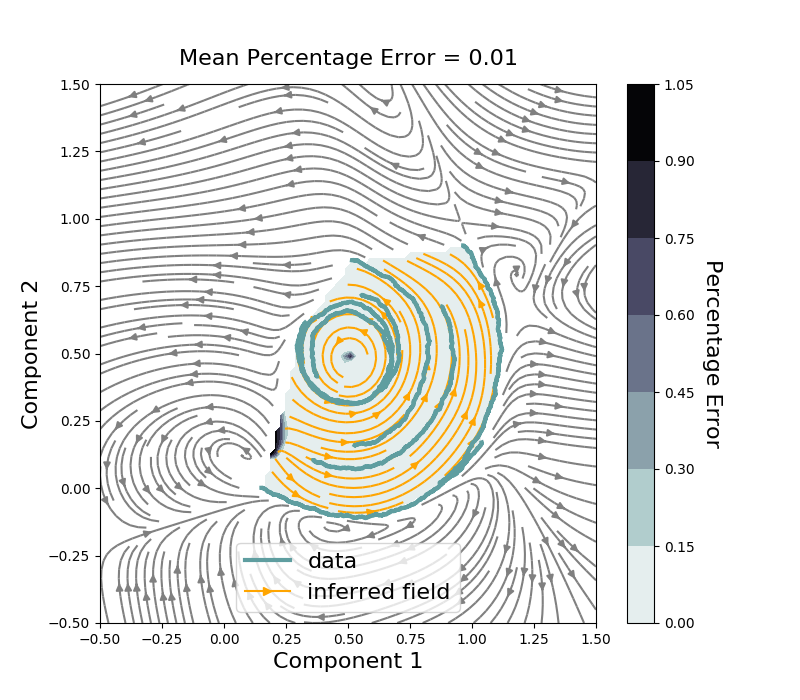
\includegraphics[width=125mm]{figures/cycle-2.png}
    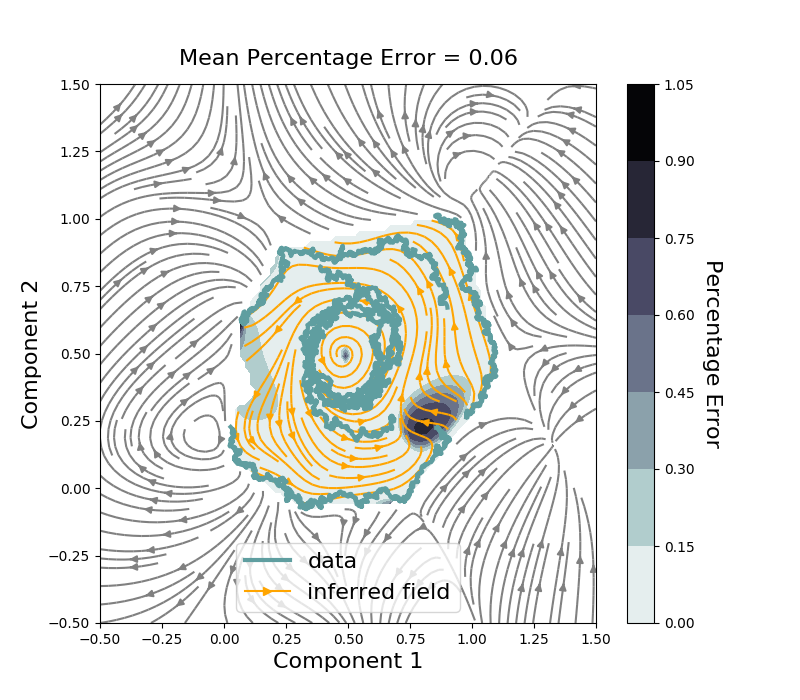
\includegraphics[width=125mm]{figures/cycle-1.png}
    \caption{Gaussian process regressors estimating derivative of the trajectories $\hat{f}$ from example trajectory datasets $\mathcal{D}_1$ ... $\mathcal{D}_K$ with varying signal to noise ratios. Interpolation error $E$ is shown as a heatmap; extrapolation fails}
    \label{fig:inferred-cycles}
\end{Figure}
The field estimate $\hat{f}$ at any given state $u$ is generated by Gaussian distributions of mean vector $\mu$ and covariance matrix $\Matrix{\Sigma}$. Solving for these requires a choice of matrix-valued kernel function $\Matrix{K}(u,v)$ which encodes our knowledge about the local structure of the field. Sophisticated kernels for learning vector fields exist \cite{Fuselier2017ADecompositions} for decomposing fields in conservative and solenoidal components, which aid in localising fixed points and cycles.

The simplest choice of kernel assumes the components are independent and have a finite correlation length $\gamma$, such as Gaussian radial basis functions. Here $\Matrix{I}$ is the identity matrix and the hyperparameter $\gamma$ has to be optimised.
\begin{equation}
    \Matrix{K}(\Vector{u},\Vector{v}) = \Matrix{I}\,\mathbb{e}^{-\gamma|\Vector{u}-\Vector{v}|^2}
\end{equation}

The second step is called \textit{matching} where the estimated field $\hat{f}$ is used as an optimisation target against some parametrised function $\rates$ with unknown parameters $\theta$.
In our setting we would like to match the geometry of the field but not its magnitude; in this sense we are focusing on the qualitative aspects of the dynamics of a set of differential equations, rather than the quantitative dynamics or kinetics. This could be achieved with the following objective function
\begin{equation}
    \mathcal{L}(\theta|\mathcal{D}) := \e^{-\frac{\hat{f}\cdot\rates}
    {|\hat{f}||\rates|}}
	\label{eq:geometric-cost}
\end{equation}
\noindent where the cost is minimal when the data derivative $\hat{f}$ and the parametrised model $\rates$ point in the same direction and maximal when they point in opposing directions.

The accuracy of the cell trajectories is limited by cell segmentation and tracking algorithms. Initial investigations into this approach also suggested that trajectories need to be of sufficient temporal resolution and sampled from a wide variety of initial conditions. Such data is not widely available and ultimately we decided to focus on a method that could be used with a well-known workhorse in biomedical research: flow cytometry.

Although we are getting close to focusing on qualitative features of a model, this objective function \eqref{eq:geometric-cost} is still sensitive to the locations and shapes of fixed point and limit cycles. What if we cared about even higher-level features such as the number of fixed points? Or perhaps whether a system oscillates or not? Bifurcation theory is well suited for this task.

\section{Afterword}
The publication in this chapter presents a method illustrating how to leverage bifurcation theory in gradient-based optimisation to obtain models that match qualitative observations. These qualitative observations are cast as constraints on structures in state space, which, as we have established in Section \ref{section:phenotypes-with-bifurcations}, also play a role in defining an organism phenotype. In the supplementary material of the incorporated publication (included here as Appendix \ref{appendix:more-complex-model}) we apply the method to infer parameters of the double exclusive reporter (Chapter \ref{chapter:double-exclusive}) against a specific width for the bistable region along one input signal, keeping the other one fixed. Surprisingly, we discovered a parameter regime that gives rise to a phenotype with damped oscillatory behaviour, which was previously unknown.

Extending the method to co-dimension two bifurcations would enable parameter inference against the whole cusp in the space of two varying inputs. While sampling the posteriors of the Monte Carlo estimates (Figure \ref{fig:double-exclusive:degradation-models}) gave us a rough indication of how robust model predictions were, the differentiability of our method would enable a more precise quantification of robustness using local sensitivity analysis.

Gradient-based optimisation is local and hence will always suffer from initialisation-specific convergence behaviour. During the development of \texttt{BifurcationInference.jl} (\texttt{github.com/gszep/BifurcationInference.jl}) a lot of effort was dedicated to ensuring that initial guesses would converge, designing hyperparameter updates between iterations and pre-conditioning of Jacobians.

Eventually, we would like to navigate \emph{equivalent} models (those that match the same qualitative behaviour) and explore the space of behaviours for a single model as part of a \emph{design--learn} workflow (Figure \ref{fig:experimental-design}--\ref{fig:non-parametric}). In order to do this, optimal parameter basins need to be explored/sampled by re-running the optimisation multiple times. This could be formalised by exploring possible probabilistic/Bayesian extensions to our method. Nevertheless, the resultant parameter distributions will be high-dimensional, introducing additional challenges of interpretation and navigation. These challenges are commonly seen in machine learning methods, but also arise frequently in the biological domain (as discussed in Section \ref{section:impute-reduce-cluster}).

In our final results chapter (Chapter \ref{chapter:exploring}), we will begin to address these challenges by introducing a tool for navigating high-dimensional point clouds in the context of flow cytometry and immunology. The high-dimensional exploration tool and its relevance in model reduction and navigation is then discussed in Chapter \ref{chapter:conclusions}.

In Chapter \ref{chapter:exploring} we find ourselves in a new application domain: immunology. Immunologists use flow cytometry on a regular basis to identify phenotypes within their datasets. We describe a computation tool leveraging machine learning approaches (described in Section \ref{section:impute-reduce-cluster}) helping immunologists to explore high-dimensional flow cytometry datasets. As with Chapter \ref{chapter:inference}, this project was a spin-out of the interdisciplinary collaboration described in Chapter \ref{chapter:double-exclusive}. In our conclusion, we speculate on the relevance of high-dimensional exploration tools in model reduction and hypothesis navigation.
\chapter{Exploring Bifurcations between Phenotypes}
\label{chapter:exploring}
\begin{music}
    \parindent10mm \instrumentnumber{1} \setstaffs1{1} 
    \generalmeter{\meterfrac44} \generalsignature{-1}
    \startextract
            \notes \ql k \Dqbl mk \ql o \ql m \en
        \bar \zw{q*}
    \zendextract
\end{music}
\epigraph{\textit{who knows what might happen to those who are consumed by greed}}{Requiem of Spirit --- Ocarina of Time}
\section{Preface}
\subsection{Problem Statement \& Context}
The studies in chapters \ref{chapter:double-exclusive}--\ref{chapter:inference} were carried out under the assumption that the underlying microscopic mechanisms that give rise to different phenotypes of an organism are known, and therefore can be modelled with differential equations that have interpretable parameters $\theta$. In section \ref{section:phenotype-inference} we outlined some popular machine learning approaches that can be used in settings where the underlying mechanism is partially or completely unknown. This chapter presents a study in immunology. While detailed models of the immune system exist \cite{Eftimie2016MathematicalDirections}, in the advent of high-throughput biology new mechanisms and exceptions are continuously being discovered \cite{Varade2020HumanChallenges}. This is done by identifying immune cell populations, their function and mechanism of action from tissue and blood samples taken from an organism in homeostasis. \emph{Immunophenotyping} methods use antibodies to identify cells based on the types of antigens or markers on their surface. As we shall see, such datasets are typically high-dimensional data clouds that can be reduced with the help of \emph{universal function approximators} and clustered to identify different immune cell phenotypes. Such high-dimensional data clouds also appear in Chapter \ref{chapter:inference} when optimal parameters $\theta$ reveal clusters of topologically or geometrically equivalent models.

In this chapter we argue the importance of interactive tools that allow immunologists to navigate high-dimensional data clouds from heterogeneous experimental setups. Such tools enable crowd-sourced consensus phenotyping of cell populations, discovery of rare populations and iterative refinement of a model of the immune system. An interactive tool \emph{FlowAtlas.jl} (\texttt{github.com/gszep/FlowAtlas.jl}) is presented in an adaptation of a manuscript being prepared at the time of writing the thesis. We conclude this chapter with a vision of how approaches in chapters \ref{chapter:inference} and \ref{chapter:exploring} can be combined to realise a high-throughput \emph{design--learn} pipeline.

\subsection{Contributions}
The following sections are an adaptation by \textbf{Grisha Szep} which deliberately omits details in the biology and experimental design in favour of thesis narrative, and will differ from the submitted manuscript. \textbf{Grisha Szep} is co-first author with \textbf{Valerie Coppard} and \textbf{Sarah Howlett}. \textbf{Joanne Jones}, \textbf{Daniel Rainbow}, \textbf{Sarah Howlett} and \textbf{Lorna Jarvis} conceived and designed the study. \textbf{Sarah Howlett}, helped by \textbf{Daniel Rainbow} and \textbf{Lorna Jarvis} acquired and processed donor tissue samples. Furthermore \textbf{Ondrej Suchanek}, \textbf{Edward J. Needham}, \textbf{Hani S. Mousa}, \textbf{David Menon}, \textbf{Krishna Mahbubani} and \textbf{Kourosh Saeb-Parsy} helped acquire and process the tissues. \textbf{Valerie Coppard} designed the flow cytometry panels, performed the experiments and exported figures from FlowAtlas and FlowJo. \textbf{Grisha Szep} conceived and implemented the computational pipeline and interactive software. All authors analysed, interpreted data and tested software.

\fakesection{Abstract}

\noindent\makebox[\linewidth]{\rule{\linewidth}{4pt}}
\begin{center}
    \Large \bfseries FlowAtlas.jl: an interactive tool bridging\\ FlowJo with computational tools in Julia
\end{center}
\noindent\makebox[\linewidth]{\rule{\linewidth}{1pt}}\\
{ \bfseries
    Valerie Coppard$^{1,3,+}$, Grisha Szep$^{2,+}$, Sarah K. Howlett$^{3,+}$, Lorna B. Jarvis$^{3}$, Daniel B. Rainbow$^{3}$, Zoya Georgieva$^{3}$, Suchanek O$^{4}$, Edward J. Needham$^{3}$, Hani S. Mousa$^{3}$, David K. Menon$^{5}$, Krishna T. Mahbubani$^{6}$, Kourosh Saeb-Parsy$^{6}$, and Joanne L. Jones$^{3}$
}\\{\footnotesize
$^{1}$Microsoft Research Cambridge, Station B, Cambridge\\
$^{2}$King's College London, Randall Centre for Cell \& Molecular Biophysics, London\\
$^{3}$University of Cambridge, Department of Clinical Neurosciences, Cambridge\\
$^{4}$University of Cambridge, Department of Medicine, Cambridge\\
$^{5}$Department of Anaesthesia, University of Cambridge, Cambridge\\
$^{6}$Department of Surgery, University of Cambridge, Cambridge\\
$^{+}$Co-first authors 
}\\
\begin{center}
\begin{minipage}{10cm}
    \noindent As the dimensionality, throughput, and complexity of cytometry data increases, so does the demand for user-friendly, interactive analysis tools that leverage high-performance machine learning frameworks. Here we introduce \emph{FlowAtlas.jl}: an interactive web application that bridges the familiar user-friendly environment of FlowJo and computational tools in Julia developed by the scientific machine learning community. We demonstrate the capabilities of FlowAtlas using a novel human multi-tissue, multi-donor immune cell dataset, highlighting key immunological findings.
\end{minipage}
\end{center}
\pagebreak

\section{Introduction}
Rapid advancements in flow and mass cytometry have brought about a new era of high-dimensional cell phenotyping \cite{Cheung2021CurrentSoftware}. However, new algorithms and computational methods for dealing with high-dimensional data are typically not accompanied by user-friendly, flexible and interactive analysis tools. The wider biomedical research community relies on intuitive and transparent analysis for reaching consensus on discoveries. The uptake of currently available computational tools by biologists remains low, likely due to the lack of inter-operability with familiar platforms such as FlowJo or FCSExpress \cite{Cheung2021CurrentSoftware} and high entry requirements for computational literacy. Here we introduce FlowAtlas -- our effort to address the following issues:

\begin{itemize}
    \item Comparing insights from immunophenotyped datasets from heterogeneous experimental designs is difficult
    \item Navigating high-dimensional data in well-established tools like FlowJo or FCSExpress is difficult
    \item Limited computational resources require down-sampling data that may contain rare populations
    \item Pipelines built in scripting languages like R or Python have limited inter-operability with FlowJo
\end{itemize}

\begin{Figure}
    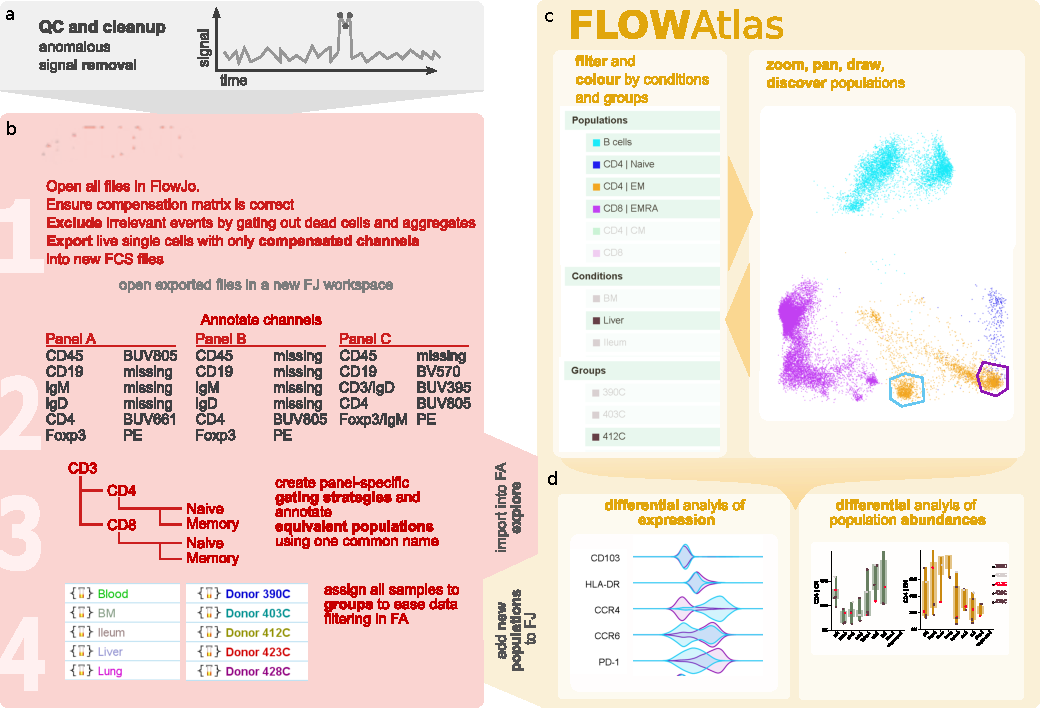
\includegraphics[width=\linewidth]{flow-atlas}
    \caption{Overview of FlowAtlas workflow with FlowJo. \textbf{a} Anomaly filtering removes instabilities in fluorescent signals. \textbf{b} Pre-processing in FlowJo includes: annotation of fluorescence channels, sample groups and cell populations with gating strategies. Importing the FlowJo workspace  into FlowAtlas triggers panel merging, embedding calculation, and launches a graphical user interface. \textbf{c} FlowAtlas enables interactive navigation of embedding. Cells can be filtered and coloured by any property defined in FlowJo. \textbf{d} Regions of interest can be drawn in the embedding to generate violin plots of marker expression. Relative frequency box plots are generated from group annotations and filter selection. Novel populations identified in FlowAtlas can be validated and annotated in FlowJo}
    \label{fig:flow-atlas}
\end{Figure}

We showcase the capabilities of FlowAtlas using a novel human flow cytometry dataset consisting of immune cells extracted from the tissues of five deceased organ donors. Immunophenotyping was performed using three slightly different antibody panels (see Tables \ref{table:donors}--\ref{table:panels} for donor metadata and panel information) representing heterogeneity in experimental design that is typical across multiple datasets. FlowAtlas was designed for use in an iterative discovery loop with FlowJo, where traditional FlowJo gating strategies provide initial annotation of main cell populations, conditions, and sample grouping to guide the discovery of new sub-populations. With the help of a high-performance visualisation library \texttt{GigaSOM.jl} \cite{Kratochvil2018RapidEmbedSOM}, we can perform a two dimensional embedding of high-dimensional datasets without down-sampling. The scatter visualisation methods from \texttt{GigaSOM.jl} were exposed to a browser front-end with interactive library OpenLayers \cite{MetaCarta2006OpenLayers}. This enabled the visual exploration and profiling of hundreds of millions of cells. By imputing missing values before dimensionality reduction, using random sampling with replacement, datasets acquired using non-identical antibody panels can be integrated and analysed together. To remove any biases induced by algorithms or data processing, the imputed values are neither visualised nor included in any downstream analysis.

\section{Proposed Method}

\subsection{Pre-processing}
When using a flow cytometer, acquisition anomalies can result from sudden flow rate or signal acquisition instability and induce undesired spearing in population distributions \cite{Lee2001HydrodynamicCytometer}. The proposed pipeline filters these anomalies using an existing method called FlowAI \cite{GianniMonaco2017FlowAI}. Filtered files are then imported into FlowJo for data pre-processing, which includes quality control of compensation matrices and gating of live lymphocytes using forward, side scatter and zombie dye channels. The resulting live lymphocytes data are then exported as new files, reducing the file size by approximately 40\%. This substantially shortens the time to carry out the computationally expensive embedding algorithm. FlowJo is then used to annotate channels and resolve discrepancies between channel names that were defined at acquisition time from different panels. In our dataset, for example, some samples only had the signal from FoxP3 while others had both FoxP3 and IgM markers in a single channel. By renaming FoxP3 to FoxP3-IgM in the relevant samples in FlowJo we can analyse both sample sets together in FlowAtlas. Missing channels between datasets are imputed only for the purposes of calculating the embedding.

\subsection{Annotation in FlowJo}
Hierarchical gating strategies (Figure \ref{fig:gating}) are used to annotate known populations of interest. These strategies can differ between samples and panels as long as gates that define the same phenotype are given the same name. Cells that fall outside of the gating strategy are annotated as \textit{unlabelled} in FlowAtlas and can still be explored. The filters that can be used to navigate and colour-code the embedding are defined by the sample group names in FlowJo. In this dataset, each sample is allocated to two groups: one telling us which tissues the sample came from, the other identifying the donor. By default, groups are interpreted as different \textit{conditions} of a sample, unless the group name contains numbers, in which case the group is interpreted as a \textit{batch}. The user can rename and rearrange groups in FlowAtlas to control this interpretation. In our dataset the \textit{conditions} are different tissues and \textit{batches} are different donors.
\begin{Figure}
    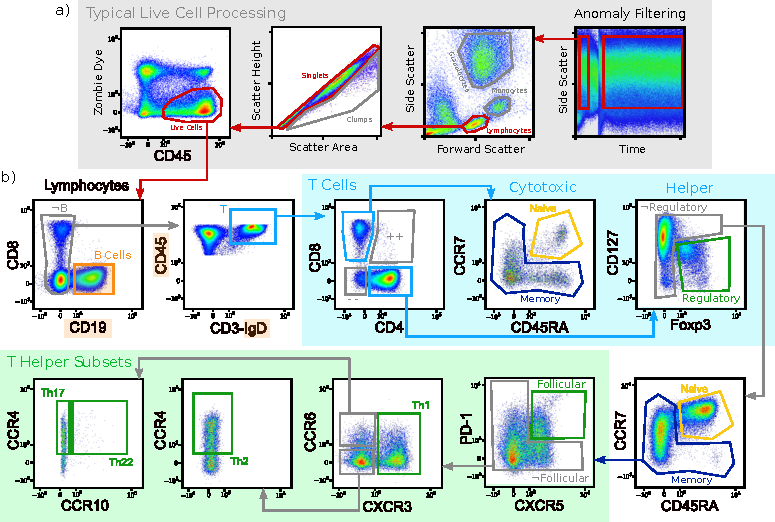
\includegraphics[width=\linewidth]{gating}
    \caption{Gating strategy for a given condition and batch. \textbf{a} A typical strategy for extracting live singlet lymphocytes, reducing the dataset size by 40\%. \textbf{b} Immunophenotyping strategy for identifying T-helper subsets. Any or all of the following channels (highlighted in orange) may be missing due to heterogeneous panel design: CD19, IgD and CD45}
    \label{fig:gating}
\end{Figure}

\subsection{Exploration in FlowAtlas.jl}
The information from the FlowJo workspace is loaded and parsed by FlowAtlas. Individual files are merged into one table and missing values are imputed for the purpose of the embedding. The embedding mapping is cached in a file named with a \texttt{.som} extension. The same mapping can be used for different datasets as long as the channel names and the total number of channels match. To re-calculate the mapping, one simply deletes the cache file. Sharing the cache file together with the FlowJo workspace and FCS files allows colleagues to work on the same embedding to verify findings in a reproducible manner. 

The graphical user interface has a map of the two dimensional embedding that was obtained by dimensionality reduction with EmbedSOM \cite{Kratochvil2020GigaSOM.jl:Datasets}. The map can be zoomed and panned and is rendered efficiently using OpenLayers \cite{MetaCarta2006OpenLayers}. The left-hand panel menu was designed with D3.js \cite{Bostock2011D3.js} and has four tabs: \textit{Annotations}, \textit{Expression}, \textit{Frequency} and \textit{Settings}. The \textit{Annotations} tab allows the user to filter and colour the embedding by marker expression, population, condition and batch information imported from FlowJo. The conditions and batches can also be redefined here. The \textit{Expression} tab has a polygon draw tool that enables gating populations directly in the embedding filtered by settings in the \textit{Annotations} tab. The gates are then used to produce violin plots that reveal fluorescence distributions across all markers. By clicking the violins it is possible to re-colour the gates to perform a differential expression analysis. The \textit{Frequency} tab generates box plots showing relative abundance of selected populations and conditions relative to any set of parent populations. The parental population, the \textit{conditions} axis and \textit{batch} marker colours are defined by settings in the \textit{Annotations} tab. Unique sub-populations identified in FlowAtlas can then be validated in FlowJo. This iterative discovery loop facilitates the identification of rare phentypes that may otherwise be missed by due to down-sampling or under-fitting in unsupervised clustering approaches.

\section{Results}
It has become common-place in single cell analysis publications to include a two dimensional embedding that reveals different cell phenotypes as clusters in the scatter plot \cite{Liu2020RecentData}. While providing a global overview of the dataset, such static images are difficult to interrogate for batch variance and possible subset structures that may imply there are unlabelled phenotypes present that were not captured by the gating strategy (Figure \ref{fig:gating}). FlowAtlas provides an interactive interface for filtering, colouring and zooming into an embedding for efficient phenotype discovery. By filtering and colouring by batch, it is possible to readily identify batch effects and subsets that are conserved across batches (Figure \ref{fig:treg-batches}). 
\begin{Figure}
    \includegraphics[width=\linewidth]{treg-batches}
    \caption{Detecting batch variance within the regulatory helper phenotype. \textbf{a} Regulatory to helper ratio by tissue aggregated over batches reveals enrichment in lymph nodes and blood. \textbf{b} Self-organised map embedding of all regulatory cells coloured by Helios expression. A region of high Helios expression can be identified and zoomed, in searched for subsets. \textbf{c} Embedding coloured and filtered by different batches to identify conserved subsets. Fluorescence distributions reveal missing channels and batch effects.}
    \label{fig:treg-batches}
\end{Figure}
Once the subsets conserved across batches have been identified they can be gated directly in the embedding (Figure \ref{fig:treg-discovery}). Filtering the embedding by tissue will give us an initial estimate for the relative abundance of the newly identified subsets. The fluorescence distributions for each gate will guide additions to the gating strategy in FlowJo.
\begin{Figure}
    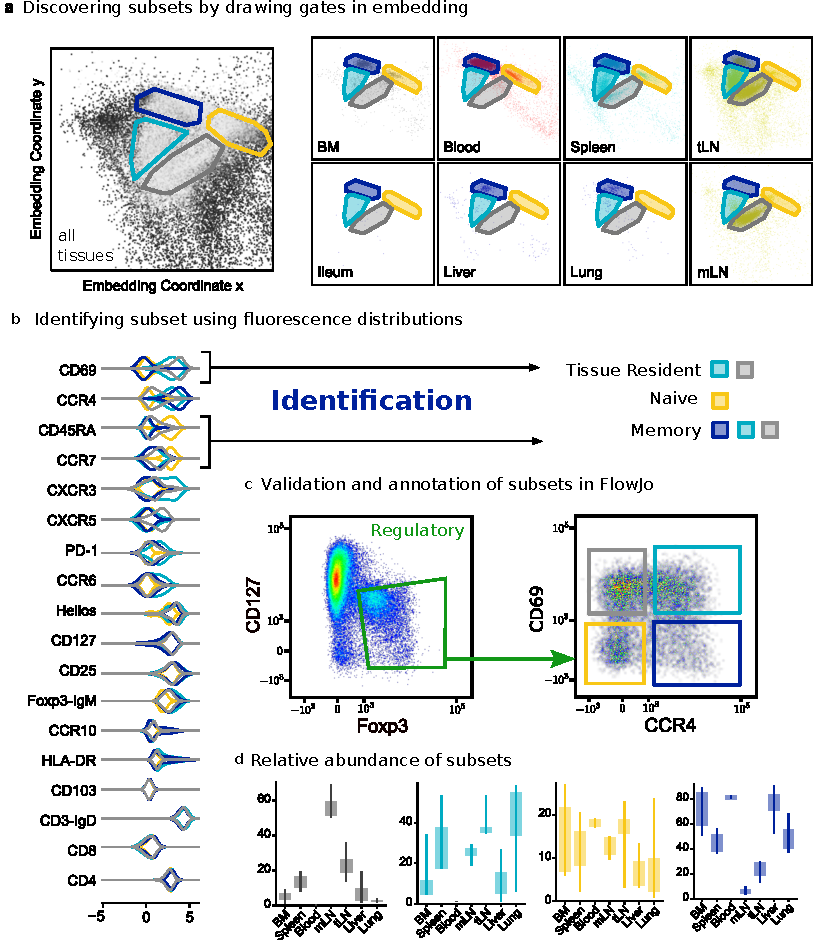
\includegraphics[width=0.9\linewidth]{treg-discovery}
    \caption{Identification of regulatory subsets. \textbf{a} Gating in the embedding and filtering by tissue reveals certain populations are not present in blood. \textbf{b} Fluorescence distributions reveal tissue resident, naive and memory phenotypes. \textbf{c} Channels that distinguish subsets can be gated in FlowJo for validation and annotation. \textbf{d} New annotations can be used to calculate relative abundance, verifying the absence of memory subsets in blood and enrichment in tissues}
    \label{fig:treg-discovery}
\end{Figure}

\subsection{Regulatory Helper Subsets}
Regulatory T helper cells suppress immune response and thereby maintain homeostasis and self-tolerance. It has been shown that regulatory helpers are able to inhibit T cell proliferation and cytokine production and play a critical role in preventing autoimmunity \cite{Kondelkova2010RegulatoryDisorders}.

In our dataset, regulatory helpers were enriched in mesenteric lymph nodes (mLN) accounting for more than 20\% of all helper cells across all donors (Figure \ref{fig:treg-batches}a). Colouring the embedding of regulatory helper cells by the expression of the Ikaros family transcription factor Helios (Figure \ref{fig:treg-batches}b) revealed Helios$^+$ and Helios$^-$ subsets as expected \cite{Thornton2019Helios:Clouds,Himmel2013Helios+Humans}. While inter-batch variability existed, the relative positions of four clusters within the Helios$^+$ subset was conserved (Figure \ref{fig:treg-batches}c). Differential expression in violin plots revealed variation due panel design: higher CD4 fluorescence intensity for one batch due to use of a different dye (Table \ref{table:panels}).

Four subsets within Helios$^+$ could be identified and gated to obtain fluorescence distributions (Figure \ref{fig:treg-discovery}b) which revealed that CD69, CCR4, CD45RA and CCR7 and explain the majority of variability between clusters. We identify one naive regulatory helper phenotype (CD45RA$^+$, CCR7$^+$) and three populations showing characteristics of the memory phenotype (CD45RA$^-$, CCR7$^-$). The memory subsets can be further subdivided in a CCR4,CD69 quadrant and verified on FlowJo (Figure \ref{fig:treg-discovery}c). Two subsets were found to express CD69$^+$, a marker of tissue residency that promotes retention through sequestration of the \emph{sphingosine-1-phosphate} receptor \emph{S1P1} required for their egress \cite{Shiow2006CD69Organs,Kumar2017HumanSites,Sathaliyawala2013DistributionSubsets}. Dividing the embedding by tissue revealed tissue-specific enrichment patterns with blood lacking the CD69$^+$ subsets consistent with their tissue residency phenotype (Figure \ref{fig:treg-discovery}d). Lung and liver contained a high proportion of regulatory helpers expressing the chemokine receptor CCR4. CCR4 has been reported to play an important role in T cell trafficking to the lung \cite{Mikhak2013LungCCR4} and in the infiltration of regulatory helpers into tumours \cite{Bromley2008OrchestratingTraffic}. 

Similar to how we've shown for regulatory T helper cells here, this iterative discovery loop can be performed for any other population of interest. We now proceed to a second example in which we explore Th1 helper cells.

\subsection{Th1 Helper Subsets}
Th1 helper cells prime the immune response against intracellular microorganisms including, viruses, intracellular bacteria, and some intracellular parasites. This is done by the secretion of cytokines, small protein mediators that activate and recruit macrophages and cytotoxic T cells to target cells to a site of infection.

\begin{Figure}
    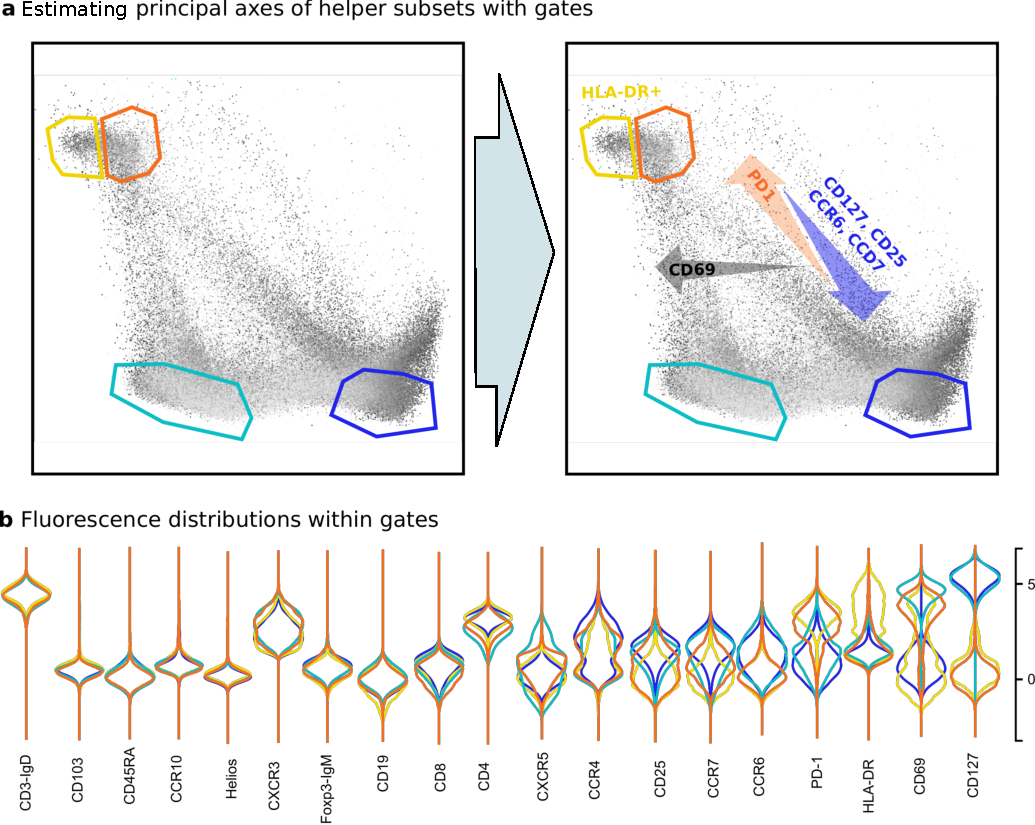
\includegraphics[width=0.9\linewidth]{th1}
    \caption{\textbf{a} Estimating the local principal axes in the embedding for Th1 helper subsets. \textbf{b} Fluorescence distributions within gates reveal correlations}
    \label{fig:th1}
\end{Figure}

An exploratory analysis of Th1 helper subsets reveals that the population distribution is supported on a simplex, whose principal axes can be constructed from correlations between fluorescence channels (Figure \ref{fig:th1}). Cells characterised by the co-expression of CD69 and CD127 are lacking blood, consistent with tissue residency.

\section{Discussion}
\label{exploring:discussion}
In conclusion, FlowAtlas brings a new iterative analysis concept to biomedical scientists by linking the familiar FlowJo workflow with a high-performance machine learning framework in a fully graphical, interactive environment. FlowAtlas allows rapid computation of embedding of millions of high-dimensional events on an average laptop without the need for down-sampling. The resulting embedding is highly interactive, offering zooming to explore deeper cluster structures, colouring and filtering of embedded events by custom conditions, the generation frequency statistics and the drawing of gates directly in the embedding for comparative analysis of marker expression. Moreover, state-of-the-art missing data handling methods enable concomitant cross-study analysis of datasets with non-identical panel designs or marker numbers. Findings can be immediately validated in FlowJo in an iterative discovery loop with FlowAtlas simplifying the identification and validation of rare or novel cell populations, which are more likely to be detected in the absence of down-sampling. FlowAtlas aims to strengthen the open-source collaborations between researchers using flow cytometry and the rapidly growing scientific machine learning community in Julia programming language.

A significant amount of time was spent adjusting the gating strategy which formed the initial annotations of different immune cell phenotypes. One point of disagreement was how sensitive biological findings and conclusions were to adjustments in the gating strategy. Sensitivity methods would resolve such issues. Furthermore, there is often disagreement between experts on how gates should be placed and what the appropriate anomaly filtering, compensation and non-linear transformation settings should be. Domain knowledge often leads immunologists to ask specific questions and annotate populations at the tails of distributions rather than their density centres. Clustering approaches, that may provide us with gating strategies automatically, typically lack the flexibility to define such populations. The immunologist wants the ability to intervene with their own annotations at any given stage of data processing.

The emerging picture suggests that building a crowd-sourced differentiable gating annotation tool would be valuable to the flow cytometry community. Community consensus annotations of large datasets are used by consumer internet businesses like Google and Microsoft on a regular basis to provide training data for their machine learning algorithms \cite{Vaughan2018MakingResearch}. Differentiability enables the application of sensitivity and optimisation methods which would be reveal the most robust annotations with highest consensus, and perhaps more importantly, reveal disagreement and ambiguity in biological findings, guiding the design of future experiments. The resolution of disagreement can be further incentivised with micro-transactions, thus potentially requiring the use of Web3 technology. The term \emph{decentralised science} \cite{Hamburg2021CallMovement} has already been coined but yet to have an established movement behind it.

The dimensionality reduction method \emph{EmbedSOM} \cite{Kratochvil2018RapidEmbedSOM} was not designed with interaction in mind. In principle it would be possible to provide continuous updates to the two dimensional embedding parameters based on the zoom and pan parameters of the field of view. Reduction methods already exist that leverage hyperbolic embeddings \cite{Peng2021HyperbolicSurvey} which allow more information from higher dimensions to be packed into a lower dimensional non-euclidean space. Combining these methods with interactive elements, perhaps even using virtual reality \cite{Reski2020OpenTechnology}, may enable researchers to gain a more intuitive grasp of high dimensional datasets by interactively zooming between global and local structures.
\chapter{Conclusions}
\label{chapter:conclusions}
\begin{music}
    \parindent10mm \instrumentnumber{1} \setstaffs1{1} 
    \generalmeter{\meterfrac64} \generalsignature{0}
    \startextract
		\notes \ql o \hl k \ql m \en \bar
              \notes \ql o \hl k \ql m \en \bar
              \notes  \Dqbl oq \ql p \ql n \Dqbl mn \en \bar
              \notes \ql o \ql k \Dqbl jl \ql k \en
    \zendextract
\end{music}
\epigraph{\textit{a childish mind will turn to noble ambition}}{Song of Time -- Ocarina of Time}

\section{Retrospectives}

In this thesis we explored the relationship between an organism phenotype and bifurcations in differential equations models seeking to model the organism behaviour. In the collaboration in synthetic biology in Chapter \ref{chapter:double-exclusive}, the experimental design goals were to engineer a particular phenotypic behaviour of \emph{E. coli}. By using a corresponding differential equation model, this design task could be explored computationally by attempting to find bifurcations. However, this led us to realise that there exists a gap in the machine learning literature, as there were no methods for differential equation models that could directly optimise for targets directly in state space. Therefore, we proposed the method described in Chapter \ref{chapter:inference}. We laid the foundations for methods that learn the parameters of differential equation models that enable qualitative behaviours and high-level constraints to be matched in state space. With this new method in hand, we revisit in this chapter how the collaboration in synthetic biology would have benefited and propose a \emph{Design-Learn} workflow that we argue would benefit any collaboration which designs phenotypes through iterative genetic manipulation of an organism \cite{Dalchau2018}. However, differential equation models for an organism behaviour are not always available, as in the collaboration in immunology in Chapter \ref{chapter:exploring}. There, we outlined the importance of interactive exploration and refinement of annotations of high-dimensional data clouds and built \emph{FlowAtlas.jl} to enable immunophenotyping across datasets with heterogeneous experimental designs. Our retrospectives are concluded with a vision of how methods from Chapter \ref{chapter:exploring} can be used together with our proposed \emph{Design-Learn} workflow to organise and reduce different models of organisms whose behaviours can be experimentally captured with flow cytometry.

\subsection{A \emph{Design-Learn} workflow for synthetic biology}

One of the main insights from our collaboration in synthetic biology is the importance of the representation of the observed data in tuning the learned aspects of a hypothesis. The data representation must be invariant under  transformations that we do not want to learn. For example, when engineering \emph{E. coli} to produce stable patterns, we did not care about the timescales or dynamical transients in the organisms response to experimental inputs. We also did not care about the exact concentrations of fluorescent proteins at steady state. The main concern was designing the shape of the bistable region in the experimental inputs.

This motivates processing flow cytometry data using basis function methods (Section \ref{section:basis-function-methods}) and running co-dimension two continuation methods to extract the limit curve that defines the separatrix between monostable and bistable regions in state space. The limit curve tells us where the steady state manifold folds, and can then be used as target data $\targets$ to infer parameters $\theta$ of some hypothesis $\rates$ using the method in Chapter \ref{chapter:inference}. Alternatively, one can optimise $\theta$ with respect to a geometric cost \eqref{eq:geometric-cost} that compares the field estimated from data $F$ to some parametrised hypothesis $\rates$. While kinetic information is ignored in this method, modes in the fluorescence distributions in the flow cytometry data define the locations of fixed points, and hence the shape of the steady state manifold. Whether design goals involve the whole shape of the steady state manifold or just its fold locations, a non-parametric representation $F$ of the data is required. Once the optimal parameters $\theta^*$ are obtained, the experimentalist can explore the neighbourhood of $\theta^*$ and see how they can change the bistable region, or whether they are close to another bifurcation which would produce a new phenotype. This can lead to new experiments that change the genotype $\theta^*+\Delta\theta$ in attempts to produce new phenotypes. Changes in genotype can involve promoter engineering for modulating transcription rates \cite{Cetnar2021SystematicOperons,Blazeck2013PromoterLevel}, using degradation tags to change degradation rates \cite{Trauth2019SyntheticProcesses} or ribosome binding site engineering for controlling translation \cite{Salis2011TheCalculator}. The new data in turn can be used to refine the hypothesis; a summary of such a \emph{Design-Learn} pipeline is presented in Figure \ref{fig:deisgn-learn}.

This pipeline should be particularly valuable for experimental design goals that are expressed in terms of qualitative statements. Rather than collecting data on time courses, which may bias learning away from the high-level design goals specified, collecting steady state information in the form of flow cytometry  
\begin{Figure}
	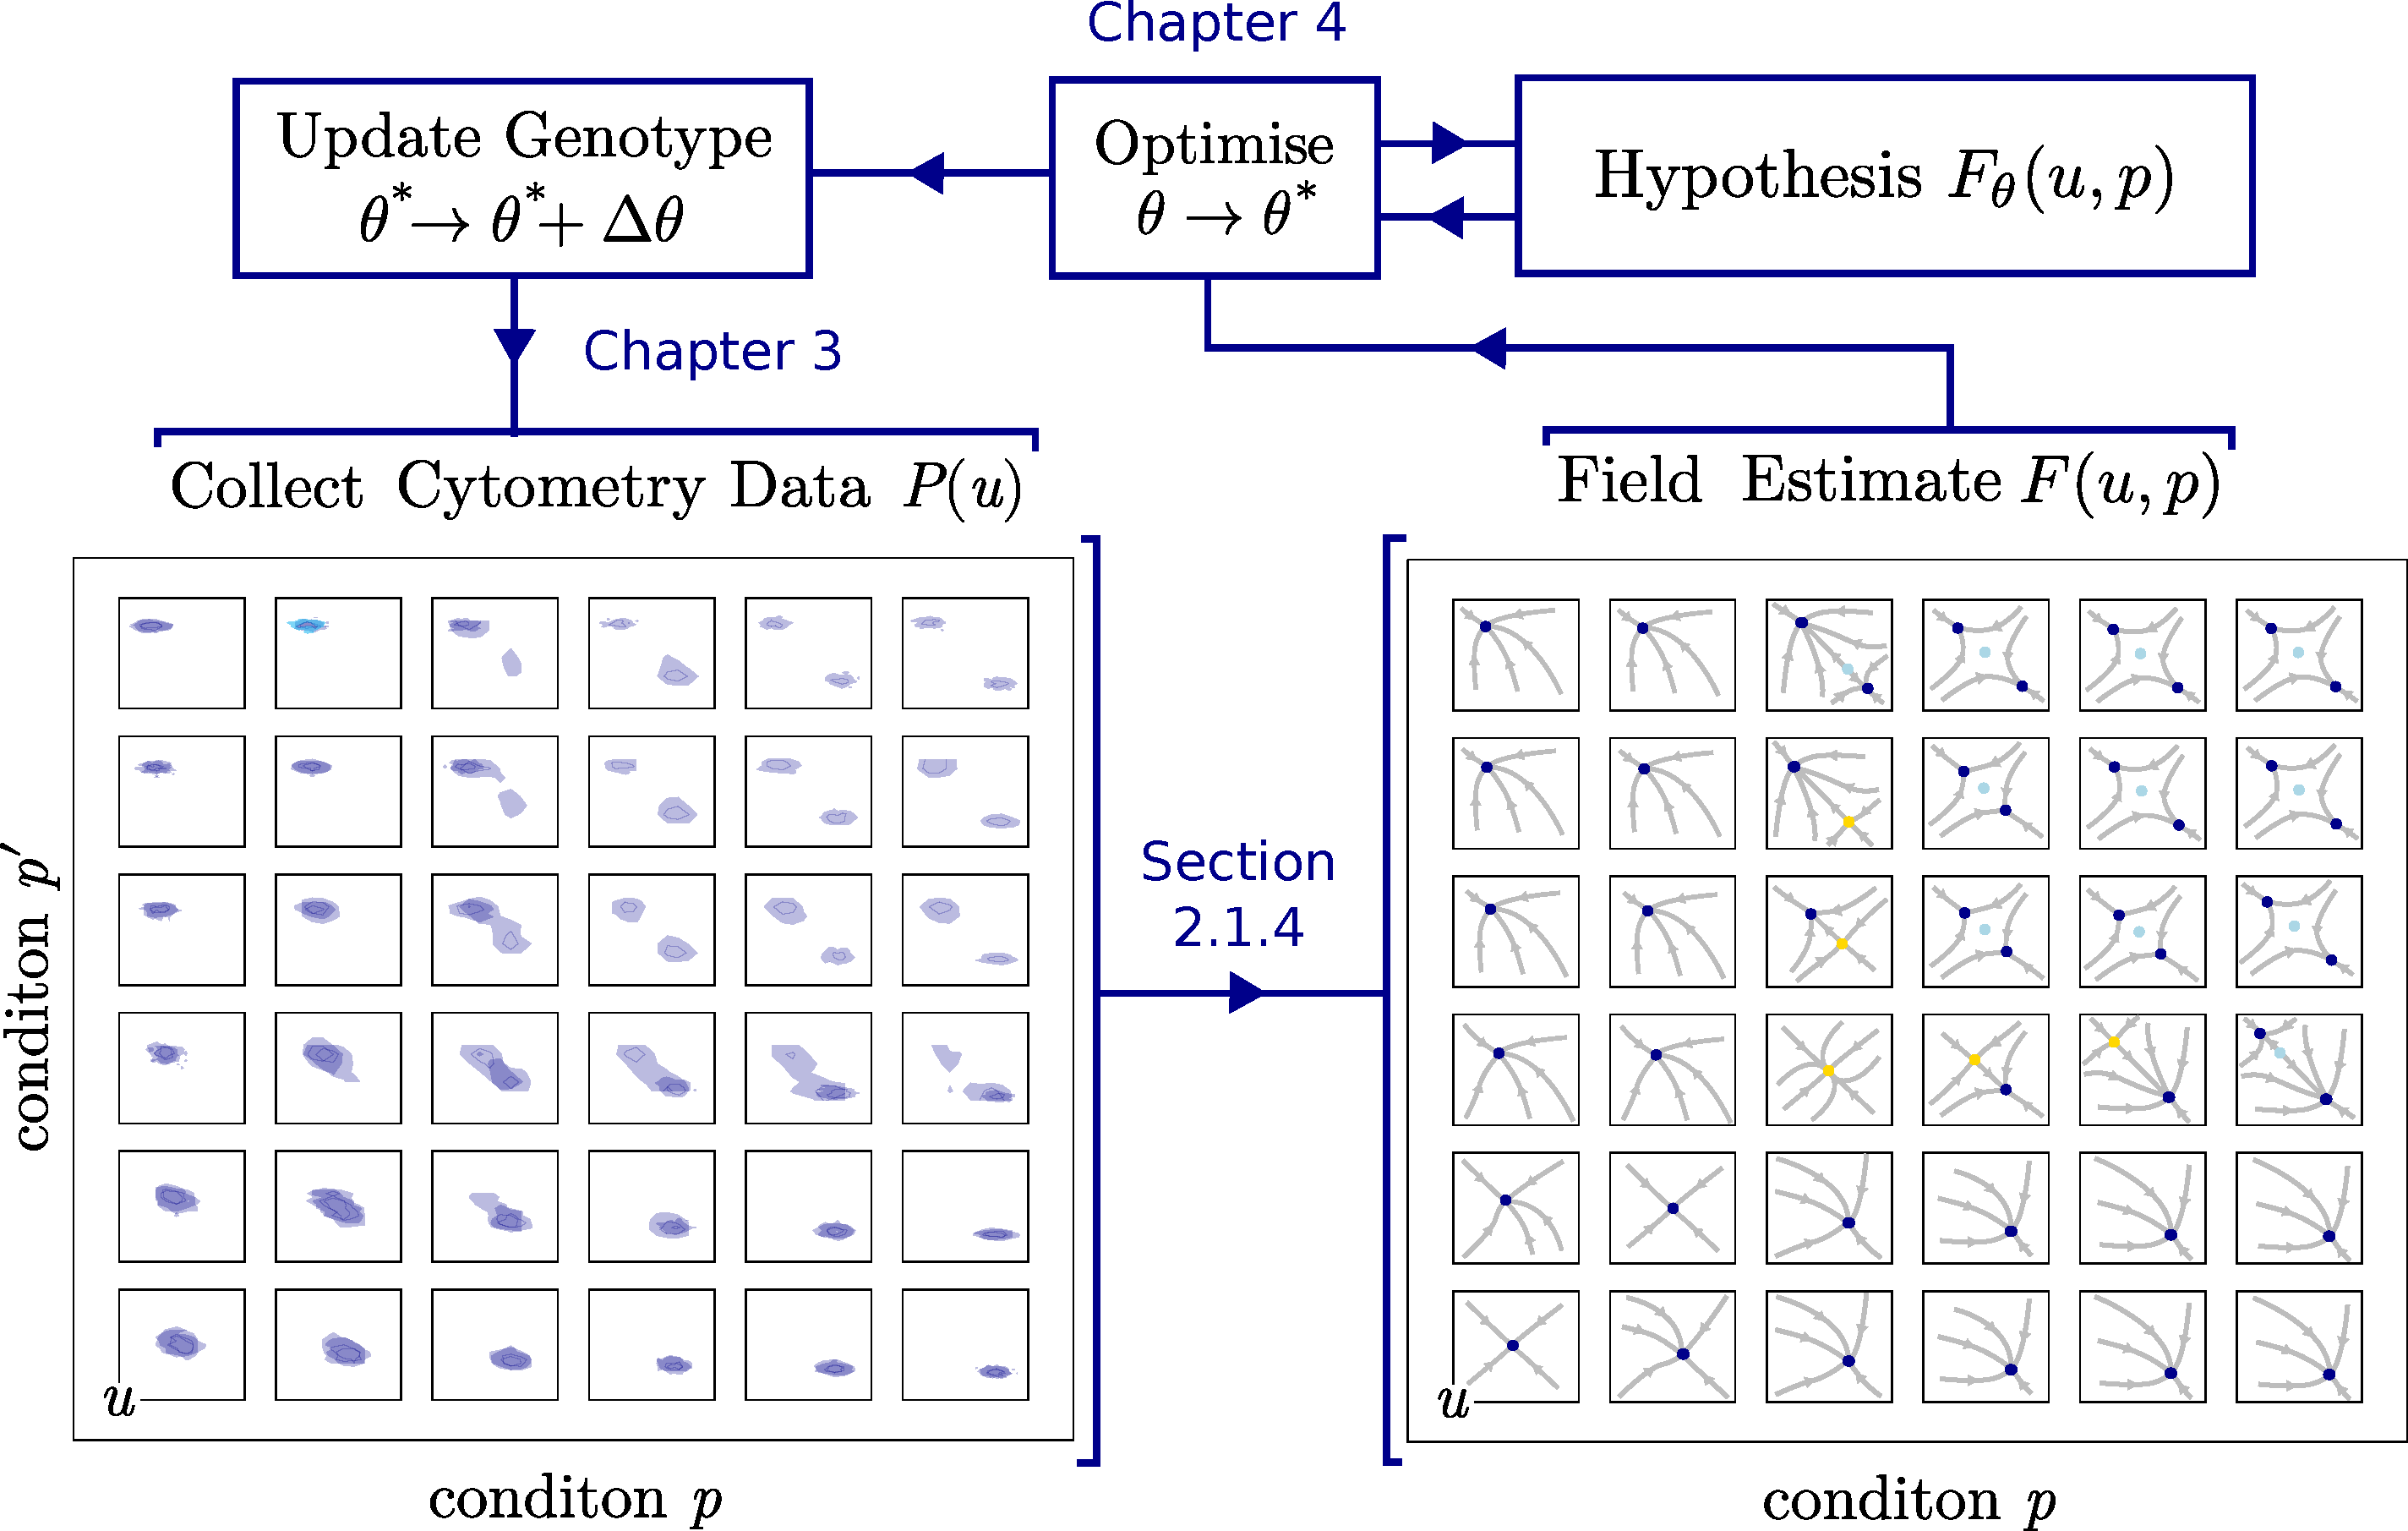
\includegraphics[width=\linewidth]{design-learn}
	\caption{Overview for a \emph{design-learn} workflow, developed in hindsight, for genetic design of the \emph{double exclusive reporter}. Non-parametric estimates of the field $F(u,p)$ yield state space geometry from cytometry data. A parametrised hypothesis $\rates(u,p)$ is then optimised against the data-driven state space geometry, to obtain optimal parameters $\theta^*$. The neighbourhood of $\theta^*$ is then investigated to decide which genetic modifications lead to improved designs, which are then tested with subsequent collection of more cytometry data.}
	\label{fig:deisgn-learn}
\end{Figure}
An alternative to reconstructing vector fields using non-parametric methods is to simply quantify variance around clusters in flow cytometry data. In the vicinity of bifurcations we expect certain scaling laws to emerge (Section \ref{section:fluctuations}) and localising bifurcations would require identifying such laws. A simple approach to this would be to localise cluster splitting, which was explored in Chapter \ref{chapter:double-exclusive} but never used to produce targets $\targets$ for optimisation. This was because accurate localisation of bifurcations using these methods require fine experimental sampling along the control condition $p$ and can ultimately be limited by intrinsic noise in the organism.

\subsection{Bifurcations \& model reduction}

In synthetic biology, the engineered genetic components inserted into a host genome can be individually modelled with biochemically reasonable assumptions and catalogued in a library of parts. Unfortunately, relatively little is known about the inner workings of the host or indeed most natural systems. The human immune system is one such natural system, which was explored in Chapter \ref{chapter:exploring}. Envisage how bifurcation theory, methods from Chapter \ref{chapter:inference}, and \ref{chapter:exploring} can be combined to explore the space of hypotheses and reduced models for mechanisms in the immune system. A reduced model can be thought of in similar terms as a Taylor expansion of a function around a specific point. The expansion has a reduced complexity compared to the original function and will have a finite region of validity around the point of expansion. Normal forms are in fact the lowest complexity expansions of a field in the vicinity of bifurcation points.

One of the simplest differential equation models of a flow cytometry dataset can be obtained by estimating a non-parametric field (Section \ref{section:basis-function-methods}) and then fitting normal forms around its bifurcations. The normal forms contain parameters that control the position and shape of bifurcations but are not biophysically interpretable. Models with biophysically interpretable parameters tend to have larger complexity and a higher-dimensional state space. Despite this we find that bifurcating regimes cover finite regions of the parameter space. Moreover, these bifurcations happen along a centre manifold \cite{Carr1981ApplicationsTheory} whose dimension is equal to the number of vanishing eigenvalues. By expanding complex models in the vicinity of bifurcations along their centre manifolds, reduced models can be obtained. The reduced models in turn can be decomposed into normal forms. Following such a procedure, in principle, it is possible to establish a mapping between the biophysically interpretable parameters of the complex model and the normal form parameters that control the geometry of state space.

\begin{Figure}
	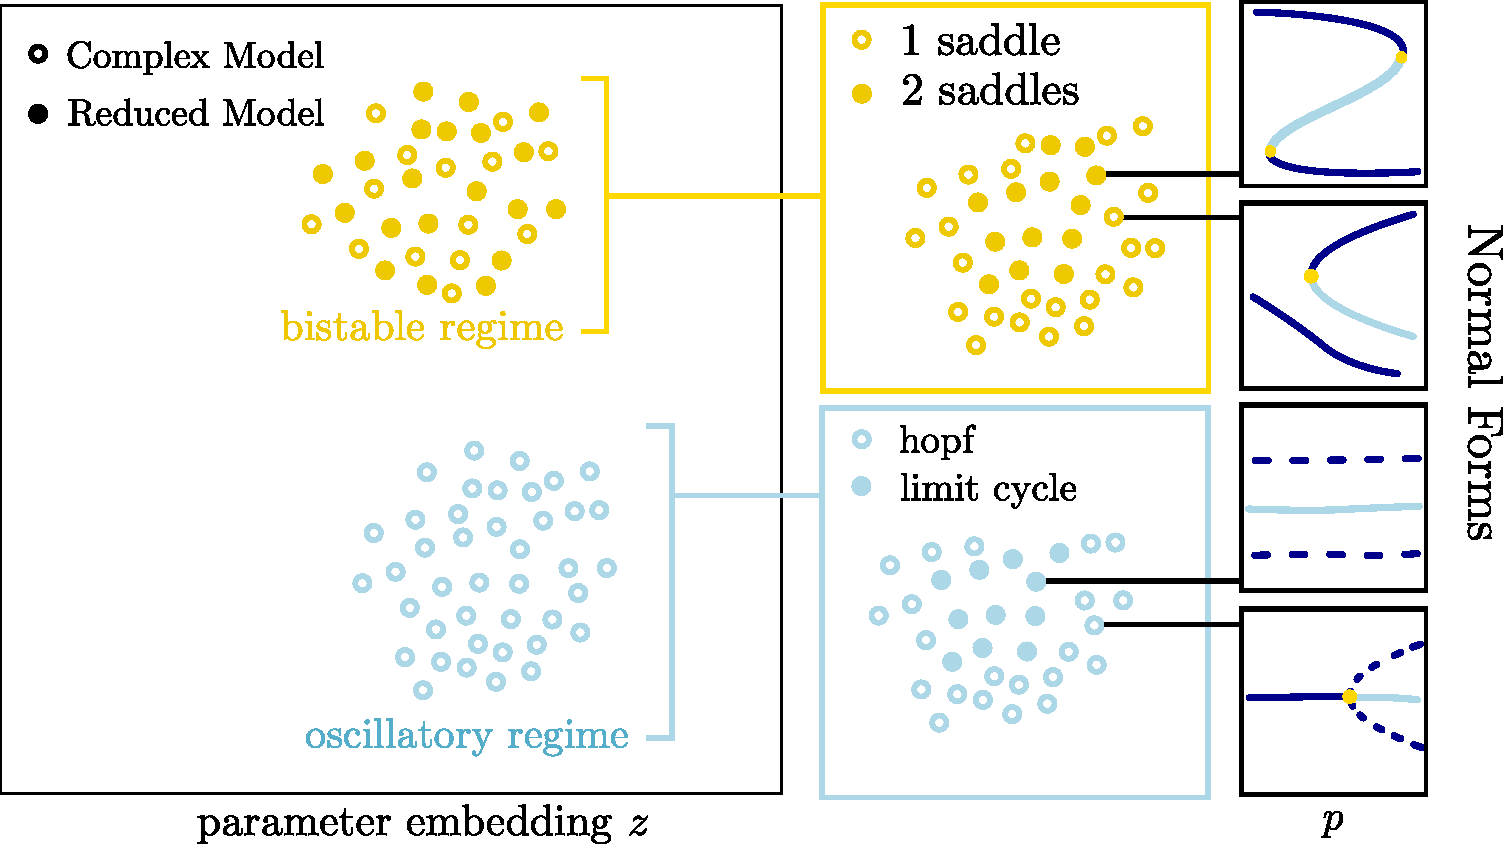
\includegraphics[width=\linewidth]{model-reduction}
	\caption{Overview of how \emph{FlowAtlas.jl} can be adapted to explore the space of models with respect to a given control condition $p$. The parameter embedding $z$ would align clusters of equivalent bifurcations in different models $\rates$, enabling the navigation of models of different complexity and discovery of reduced models}
	\label{fig:model-reduction}
\end{Figure}

Although we built \emph{FlowAtlas.jl} to navigate high-dimensional cytometry data, it can easily be re-applied to navigate any high-dimensional point clouds. Such point clouds emerge during optimal parameter estimation in Chapter \ref{chapter:inference}. In this setting, each point represents a different set of parameters $\theta$ for the given model $\rates$ and each cluster represents a set of equally valid parameters that qualitatively match a given dataset $\targets$. Now suppose there are many possible models $\rates$, each with a different dimensionality of $\theta$. How can we navigate the space of models with variable dimensionality? One option is to embed them in the same latent space, as we did with flow cytometry datasets with heterogeneous experimental designs in \emph{FlowAtlas.jl}. This embedding would be designed to map clusters that contain the same bifurcations for different models onto the same cluster in the latent space. Such a mapping would allow colouring and filtering a common embedding by model and bifurcation type, enabling navigation of model space (Figure \ref{fig:model-reduction}) and discovering reduced models for complex flow cytometry datasets.

\section{Limitations}

In this thesis we focused on a subset of optimisation algorithms that make us of local gradient information. While this approach has been widely successful in machine learning and deep learning applications over the past decade \cite{Bronstein2021GeometricGauges} results may be highly dependent on initialisation and/or pre-conditioning. Notably, our method in Chapter \ref{chapter:inference} suffers from the same gradient instabilities with respect to ill-conditioned systems as other implicit layer approaches \cite{Kim2021StiffEquations}.

We emphasised the importance of obtaining regions and distributions of parameters and models rather than individual data points. Therefore, throughout this thesis we have been estimating distributions with multiple re-runs of the optimisation. However, this can be computationally expensive and have no guarantee that all regions of the distribution have been properly sampled. Global optimisation methods, for example leveraging interval arithmetic \cite{Kjller2007Non-linearPropagation}, can provide us with guaranteed solutions within a particular region, but can be even more computationally demanding, and have only been applied to very low-dimensional differential equation problems.

Another limitation of our method in Chapter \ref{chapter:inference} is that there is no natural way of encoding prior knowledge in the parameters, as is the case with Bayesian methods. For example, if we know that all parameters in the differential equation have to be positive, at the moment we are forced to log transform the parameters before passing them to the optimisation. Encoding constraints via prior probability distributions is more simple than bespoke preprocessing of parameters. Developing a Bayesian version of the underlying problem could therefore help to unify data, design goals and prior knowledge into a more adaptable method.

\section{Future Work}

We now discuss future directions that would use this thesis as a starting point. In particular, we continue the discussion of limit cycle design with basis function methods (Section \ref{section:basis-function-methods}) and the extended bifurcation measure (Figure \ref{fig:hopf-measure}). We will see how in principle it is possible to design limit cycles whose sets are defined implicitly. We then conclude with how these approaches can be used to design spatially extended systems, in particular Turing bifurcations in self organised patterns and transitions to turbulence in fluid flows.

\subsection{Designing Limit Cycles}

Designing limit cycles requires two global constraints: a closed surface $\partial\Omega$ specified in the state space $u$ and an angular momentum field $\omega(u)$ that gives rise to circulating trajectories along the surface $\partial\Omega$. Basis function methods (Section \ref{section:basis-function-methods}) naturally give rise to an unstable focus that pushes trajectories towards the limit cycle from within the surface $\partial\Omega$. We can perform gradient descent against the geometric cost function \eqref{eq:geometric-cost} using the non-parametric field in the vicinity of the limit cycle as a target. This designs the shape of the limit cycle, but not the bifurcations that created it. Therefore, by combining the geometric cost \eqref{eq:geometric-cost} with the bifurcation measure (Figure \ref{fig:hopf-measure}), we can simultaneously design the shape of the limit cycle as well as the bifurcations around it. 

\begin{Figure}
	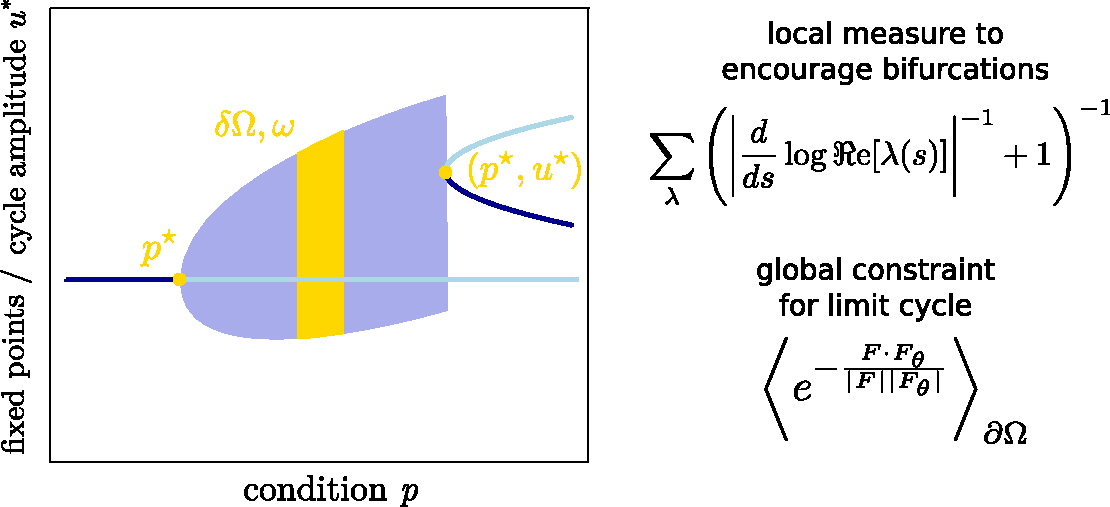
\includegraphics[width=9cm]{design-limit-cycles}
	\caption{Using global constraints $\partial\Omega,\omega$ (gold region) with basis functions in state space $u$ and local constraints at $p^\star,u^\star$ (gold point) can help design global bifurcations of limit cycles}
	\label{fig:design-limit-cycles}
\end{Figure}

As an example, suppose we would like to design a limit cycle that emerges from a local Hopf bifurcation from the left and disappears in a global infinite period bifurcation from the right (Figure \ref{fig:design-limit-cycles}). In principle we could use the bifurcation measure (Figure \ref{fig:hopf-measure}) to encourage Jacobian eigenvalues crossing the imaginary axis $\Real[\lambda]=0$ at local points $(p^\star,u^\star)$ and hope that a limit cycle appears in between them. However this could merely result in a model with two saddle node bifurcations, yielding a bistable region in between the two points $p^\star$. In order to guarantee a limit cycle we specify create a non-parametric field $F$ with global constraints $\partial\Omega,\omega$ and include it in a geometric cost. Note that we only need to evaluate the model to be optimised $\rates$ in the vicinity of the limit set $\partial\Omega$ and in principle this can be done sparsely so save compute time. The key takeaway is that by combining local constraints via Jacobian eigenvalues and global constraints via basis functions in state space, it is possible to design global bifurcations (Section \ref{section:global-bifurcations}).

\subsection{Spatially Extended Systems}

Bifurcations could also be designed in spatially extended systems. We have seen that partial differential equations can be discretised, yielding high-dimensional ordinary differential equations. This yields eigenvalue distributions (Section \ref{section:eigenvalue-distributions}) that dictate the stability of different spatial modes. Our method in Chapter \ref{chapter:inference} can be applied to the discretised equations to design snaking \cite{Uecker2021ContinuationExperiments} and hence spatial patterning regimes like spots and stripes. Solving for the bifurcation diagram of partial differential equations would not be an issue since \texttt{BifurcationKit.jl} \cite{Veltz2020BifurcationKit.jl} was originally designed to deal with this. The gradient calculation --- which would scale like $(NK)^2$ where $N$ is the number of states and $K\gg 1$ the number of spatial discretisations --- would be the limiting factor, and would have to be optimised, possibly using sparse tri-diagonal matrix methods. Local bifurcations only occur when eigenvalues cross the imaginary axis and thus further speed-up can be obtained by restricting the eigensolver to the vicinity of the imaginary axis.

Instead of discretising spatial derivatives, it is also possible to make use of the Fourier transform and linearisation of local terms, yielding dispersion relations \eqref{eq:dispersion-relation}. Dispersion relations satisfy implicit scalar equations, and hence their gradients can be obtained via the implicit function theorem. Following the strategy used by implicit layers \cite{Look2020DifferentiableLayers} we can use dispersion relations in different patches of state space as constraints for designing spatial patterns and \emph{Turing} bifurcations.

In principle, replacing eigenvalue calculations with finite time Lyapunov exponents (Section \ref{section:lyapunov-exponents}) would enable designing the onset of chaos and strange attractors. Unfortunately, computing these exponents and their gradients would be prohibitively expensive due to high dimensionality and sensitivity to initial conditions. Although, dimensionality reduction methods such as proper orthogonal decomposition \cite{Khlopov2016AutomaticDecomposition} could provide us with reduced models that may act as computationally tractable surrogates. Further theoretical investigations are required to determine whether a field such as computational fluid dynamics can benefit from inverse bifurcation analysis, but there are numerous more mature applications that could exploit such a capability, including aircraft and land vehicle design.
\addcontentsline{toc}{chapter}{Appendices}
\appendix

\chapter{Eigenvalue Distributions of Derivative Operators}
\label{appendix:eigenvalue-distributions}
Using the Circular Diagonalization Theorem \cite{Ingleton1956TheMatrices} one can derive the eigenvalues $\lambda_k$ of an $K\times K$ matrix which represents the second-order central difference approximation to the second derivative on $K$ sites of a one dimensional ring
\begin{align}
	\frac{\partial^2}{\partial x^2} \rightarrow
	\begin{pmatrix}
	  -2 & 1 &  &  &  & 1 \\
	  1 & -2 & 1 &  &  &  \\
	  & 1 & \ddots & \ddots &  & \\
	  & & \ddots & \ddots & 1 & \\
	  & & & 1 & -2 & 1 \\
	  1 & & & & 1 & -2 \\
	\end{pmatrix}\\
	\begin{matrix}
	  \lambda_k =2\left(\cos\left(\frac{2\pi k}{K}\right)-1\right) \\
	  k\in\{0,1,\cdots,K-1\}
	\end{matrix}
	\qquad
\end{align}
As the number of sites $K\rightarrow\infty$ the argument $k/K\in[0,1]$
and the eigenvalues remain bounded $-4<\lambda_k<0$. By shifting and scaling
the index $k\rightarrow\frac{k-K\pi}{2\pi}$ the eigenvalues are expressed as
a dispersion relation
\begin{align}
  \lambda(k)&=
  -2\left(\cos k+1\right)
  \quad k\in[-\pi,\pi]
\end{align}
The discrete $L$-dimensional Laplacian is simply the Kronecker sum $\oplus$ of one
dimensional cases and thus its eigenvalues are simply the sum over one dimensional dispersions \cite{Laub2004MatrixEngineers}
\begin{align}
  \lambda(k)&=
  -2\sum_{i=1}^L\left(\cos k_i+1\right)
  \quad k\in[-\pi,\pi]^L
\end{align}
The probability density $P(\lambda)$ can be expressed as a density integral
over the $L$-dimensional hypercube region $[-\pi,\pi]^L$
\begin{align}
	P(\lambda')&=\frac{1}{Z}\int_{[-\pi,\pi]^L}\!\delta(\lambda'-\lambda(k))\,\mathrm{d}k
\end{align}
We proceed with an element-wise change of variables $u=2\cos k$ and recognise that the integration region is $L$-fold symmetric across each component axis, which allows restriction of the domain of integration to a hyper-octant. In coordinates $u$ the region becomes $[-2,2]^L$
\begin{align*}
  P(\lambda)&=\frac{1}{Z}
  \int_{\Omega'}\!
  \frac{\delta(\Lambda_L+\sum_{i}u_i)}
  {\sqrt{\prod_{i=1}^L(1-u_i^2/4) }}
  \,\mathrm{d}u
  \qquad
  \begin{matrix}
    \Lambda_L=\lambda+2L \\
    |\Lambda_L|\leq2L
  \end{matrix}\\
  &=\frac{1}{2\pi Z}
  \int_{-\infty}^{\infty}\int_{\Omega'}\!
  \frac{\mathbb{e}^{\Lambda_L Ik}\exp[\sum_{i}u_i Ik]}
  {\sqrt{\prod_{i=1}^L(1-u_i^2/4) }}
  \,\mathrm{d}u\mathrm{d}k\\
  &=\frac{1}{2\pi Z}
  \int_{-\infty}^{\infty}\mathbb{e}^{\Lambda_L Ik}
  \prod_{i=1}^L\int_{-2}^{2}\!
  \frac{\mathbb{e}^{u_i Ik}}
  {\sqrt{1-u_i^2/4}}
  \,\mathrm{d}u_i\mathrm{d}k
\end{align*}
The Fourier representation of the delta function allowed the
factorisation of the integral. We recognise a repeated Bessel integral and replace it with the Bessel function of the first kind $J_n(k)$, leaving only a Fourier transform which we define as $\mathcal{F} : f\rightarrow \frac{1}{\sqrt{2\pi}} \int_{-\infty}^{\infty}f(k)e^{ I\Lambda k}\mathrm{d}k$
where
\begin{equation*}
    f(k) = \frac{1}{\sqrt{2\pi}Z}\prod_{i=1}^L\int_{-2}^{2}\!
  \frac{\mathbb{e}^{u_i Ik}}
  {\sqrt{1-u_i^2/4}} \mathrm{d}u_i
\end{equation*}
To clean the formula up even further we may use the convolution theorem to deal with the powers of $L$, leaving only the Fourier transform of the Bessel function $J_0(k)$, which is the arcsine distribution $\alpha(\lambda)$. The eigenvalue density of a Kronecker sum of matrices is the convolution of the densities of those matrices.
\begin{align}
  P(\lambda)=\underbrace{
  \alpha(\lambda)*\alpha(\lambda)*\cdots*\alpha(\lambda)}_{L}\qquad\qquad\label{eq:mlap}\\
    \alpha(\lambda)=
      \frac{\Pi\left(\frac{\lambda+2}{2}\right)}{2\pi\sqrt{1-\left(\frac{\lambda+2}{2}\right)^2}}
    \qquad
    \Pi(x)=
      \begin{cases}
        1 & |x|<1\\
        0 & |x|\geq1\\
      \end{cases}
	\label{eq:laplacian-distribution}
\end{align}
\begin{Figure}
    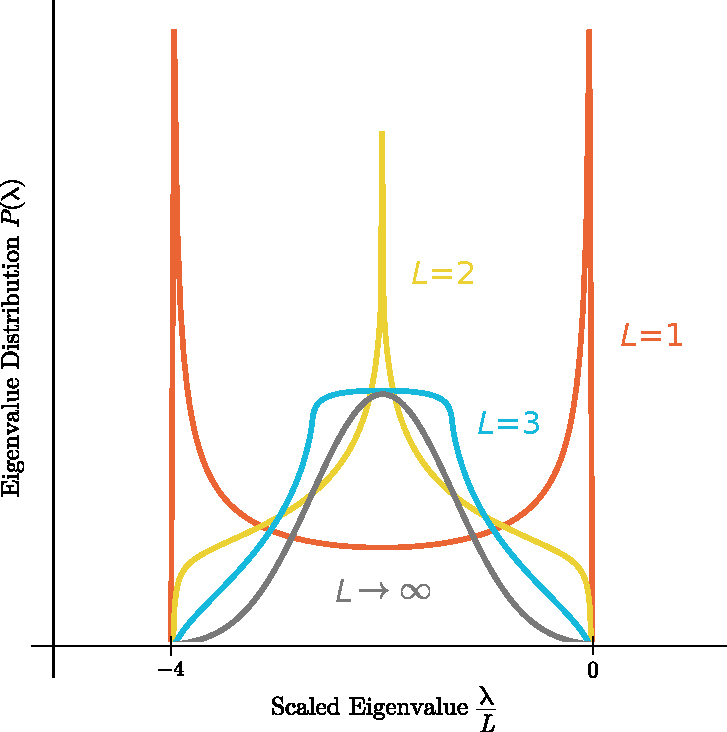
\includegraphics[width=0.6\linewidth]{laplacian-spectra}
    \caption{Eigenvalue distributions $P(\lambda)$ of the $L$-dimensional Laplacian}
    \label{fig:laplacian-spectra}
\end{Figure}
The one dimensional density has two Van Hove singularities at $\lambda=-4,0$ given by the arcsine law $\alpha(\lambda)$, whereas the two dimensional case has one at $\lambda=-4$ given by the complete elliptic integral of the first kind $K(m)$. Figure \ref{fig:laplacian-spectra} reveals that in higher dimensions singularities do not occur; instead there appear to be discontinuities in the higher order derivatives. The density smooths out as repeated convolutions bring it to a normal distribution; this is another way to state the Central Limit Theorem. In the context of diffusion, the Laplacian is scaled by the diagonal diffusion matrix. To take this scaling into account, components $D_i$ are introduced in the arcsine laws
\begin{align}
	\alpha(\lambda) \rightarrow \frac{1}{D_i}\alpha(\lambda/D_i)
\end{align}
The eigenvalue distributions determine the eigenbasis evolution  \eqref{eq:eigenbasis-vector-evolution} which reveals that the second order derivative leads to exponential relaxation of all basis vectors, except for the subset with vanishing eigenvalue $\lambda=0$. The corresponding zero eigenvectors $v_0$ are the Fourier components of the steady state distribution, and are the only components that remain as $t\rightarrow\infty$. The diffusive components $D_i$ determine the timescale of relaxation in each dimension.


\chapter{Interpretation of Morphogen Gradients by a Bistable Circuit}
\label{appendix:double-exclusive}
\includepdf[pages=1-51, offset=75 -90, scale=0.85, frame,
        clip,trim=20mm 5mm 20mm 15mm,
        pagecommand={}, addtotoc={
                2,section,1,Supplementary Figures,appendix:double-exclusive:figures,
                18,section,1,Supplementary Methods,appendix:double-exclusive:methods,
                19,subsection,2,Differential Equation Models \& Parameter Inference,appendix:double-exclusive:inference,
                40,subsection,2,Bistability Analysis,appendix:double-exclusive:bistability,
                42,subsection,2,Boundary Experiments,appendix:double-exclusive:boundaries,
                50,subsection,2,Models of the Exclusive Receiver Relay Circuits,appendix:double-exclusive:relay},
        addtolist={
                2, figure, {\textit{Supplementary Figure 1}\quad Circuit variants}, fig:double-exclusive:variants,
                4, figure, {\textit{Supplementary Figure 2}\quad Raw timecourse fluorescence traces}, fig:double-exclusive:plate-data,
                15, figure, {\textit{Supplementary Figure 13}\quad Hysteresis flow cytometry experiments}, fig:double-exclusive:flow-hysteresis,
                41, figure, {\textit{Supplementary Figure 25}\quad Bifurcation curves for uniform and protected degradation models}, fig:double-exclusive:degradation-models,
                41, figure, {\textit{Supplementary Figure 26}\quad Bifurcation curve insensitivity specific growth rate $\gamma_0$}, fig:double-exclusive:growth-rate-sensitivity
}]{publications/double-exclusive-si.pdf}

\chapter{Parameter Inference with Bifurcation Diagrams}
\label{appendix:inference}
\includepdf[pages=1-6, offset=75 -90, scale=0.85, frame,
        clip,trim=33mm 20mm 33mm 20mm,
        pagecommand={}, addtotoc={
                1,section,1,Bifurcation Diagrams as Tangent Fields,appendix:tangent-fields,
                2,section,1,Bifurcation Measure Properties,appendix:bifurcation-measure,
                3,section,1,Leibniz Rule for Space Curves,appendix:leibniz-rule,
                5,section,1,Application to the Double Exclusive Model,appendix:more-complex-model,
                6,section,1,Extension for Hopf Bifurcations,appendix:hopf-measure},
        addtolist={
                1, figure, {\textit{Supplementary Figure 1}\quad Two implicit surfaces $f_{\theta}(z)=0$ and $g_{\theta}(z)=0$ in $\mathbb{R}^3$ intersecting to form a space curve which is tangent to field $\tangent(z)$ and perpendicular to gradients $\partial_{z}f_{\theta}$ and $\partial_{z}g_{\theta}$}, fig:implicit-surfaces,
                2, figure, {\textit{Supplementary Figure 2}\quad Left/Right : Determinant $\Det$ and tangent field $\tangent(z)$ for the saddle-node/pitchfork models for some set values of $\theta$ revealing that $\Det=0$ defines bifurcations}, fig:determinant-field,
                5, figure, {\textit{Supplementary Figure 3}\quad Bifurcation inference for the \emph{double exclusive reporter}. A. Optimal parameter estimates $\theta^*$ for the targets $\targets=\{1,2\}$ (indicated by yellow lines in panel B) reveal four regions  with two geometrically different regimes: mutual activation (region 1) and mutual inhibition (regions 2-4). B. Example bifurcation diagrams indicate that region 2 has swapped kinetics between $L$ and $T$ to region 3. Region 4 has models with non-zero imaginary parts to eigenvalues indicating damped oscillations (shown in light green).},
                fig:double-exclusive-optima,
                6, figure, {\textit{Supplementary Figure 4}\quad Bifurcation measure $\measure(s)$ and eigenvalues $\lambda(s)$ along the arclength $s$ for two different bifurcation curves demonstrating how the measure detects non-zero imaginary parts $\Imag[\lambda]$ (onset of damped oscillations marked by circle) and sign changes in real parts $\Real[\lambda]$ (Hopf bifurcations marked by stars)},
                fig:hopf-measure
}]{publications/bifurcation-inference-si.pdf}

\chapter{Exploring Bifurcations between Phenotypes}
\label{appendix:exploring}

\section{Experimental Methods}
\subsection{Tissue Acquisition \& Dissociation} 

All samples were collected via the \href{https://www.cbtm.group.cam.ac.uk}{Cambridge Biorepository for Translational Medicine} under Research Ethics Committee approval 15/EE/0152. Tissue was obtained from five deceased organ donors following circulatory death. Donor metadata is given in Table \ref{table:donors}. Briefly, following cessation of circulatory function donors proceeded to organ donation. Organs were perfused \emph{in situ} with cold organ preservation solution and cooled with topical application of ice. Samples for the study were obtained within 60 minutes of cessation of circulation and placed in University of Wisconsin organ preservation solution for transport at 4°C to the laboratory. Lung and liver samples were obtained from the left lower lobe of the lung and the right lobe of the liver. In addition, two donor-matched blood samples were collected prior to withdrawal of life support, under approval 97/290.

To minimise the possibility of processing-depended differences in cell surface marker expression, all samples, including blood, were processed using enzymatic digestion protocol. Briefly, solid tissues were weighed, transferred into 10cm tissue culture dishes and cut into small pieces. Up to 5g of tissue was then transferred to each of eight GentleMACS C tubes (Miltenyi Biotec) containing 5mL of dissociation media composed of X-vivo15 supplemented with 0.13U/mL Liberase TL (Roche), 10U/mL Benzonase nuclease (Millipore/Merck), 2\% (v/v) heat-inactivated fetal bovine serum (FBS, Gibco), penicillin (100 U/ml, Sigma-Aldrich), streptomycin (0.1 mg/ml, Sigma-Aldrich), and 10mM HEPES (Sigma Aldrich). The samples were then dissociated on a GentleMACS Octo dissociator (Miltenyi Biotec) running a protocol that provided gradual ramping up of homogenisation speed and two 15 minute heating/mixing steps at 37°C. Digested tissue was passed through a 70$\mu$m MACS Smartstrainer (Miltenyi Biotec) and the flow-through was first washed with media supplemented with 2 mM EDTA and then with PBS. Mononuclear cells were enriched by Ficoll-Paque (GE Healthcare) density centrifugation according to manufacturer's instructions. Following, density centrifugation, mononuclear layer was collected, washed once with PBS and cell pellet was resuspended in FACS buffer (PBS, 2.5$\%$ FBS).

Bone marrow aspirates and peripheral blood samples were first subjected to Ficoll-Paque density centrifugation, according to manufacturer's instructions, the mononuclear layer was then collected, washed with PBS and cells were treated with the same dissociation media as solid tissues for 30 min at 37°C prior to washing and resuspension in FACS buffer.

\subsection{Flow Cytometry}

Depending on the cell yield, up to 1x10\textsuperscript{6} mononuclear cells/tissue were stained with antibodies shown in Table \ref{table:panel}. Not all donors were stained with the same panel. To expand total number of markers, sentinel panel design was implemented where CD3 and IgD were detected with antibodies conjugated to BUV395 and Foxp3 and IgM were detected with antibodies conjugated to PE in some donors. Refer to Table \ref{table:panels} for details. 

Single cell suspensions were washed once in PBS, transferred into 96 v-bottom plate and stained with Zombie UV viability dye for 30 min at 4°C following by a wash with FACS buffer. Cell pellets were resuspended in 50$\mu$l FACS buffer with Human FcR block (BD Biosciences) and incubated for 10 min at 4°C. Next, cells were pelleted, excess buffer removed and 100$\mu$l of antibody master mix composed of cell-surface antibody cocktail (see Table \ref{table:panels}), BV buffer (BD) and True-Stain Monocyte Blocker (Biolegend) and incubated for 1h at 4°C. Following incubation, cells were washed three times in PBS and prepared for intracellular staining using transcription factor fixation/permeabilisation kit (eBioscience) according to the manufacturer's instructions. Following IC staining, cell were resuspended in PBS and analysed on BD FACSymphony A3 cell analyser within 10 hours.

\section{Supplementary Tables}

\begin{landscape}
\begin{table}
\footnotesize
\begin{center}
\begin{tabular}{>{\centering\arraybackslash}p{0.6cm}>{\centering\arraybackslash}p{0.4cm}>{\centering\arraybackslash}p{0.7cm}>{\centering\arraybackslash}p{0.9cm}>{\centering\arraybackslash}p{0.9cm}>{\centering\arraybackslash}p{0.9cm}>{\centering\arraybackslash}p{1cm}>{\centering\arraybackslash}p{1cm}>{\centering\arraybackslash}p{1cm}>{\centering\arraybackslash}p{1cm}>{\centering\arraybackslash}p{2.1cm}>{\centering\arraybackslash}p{0.6cm}}
    \toprule
    Donor ID & Sex & Age & Primary cause of death & Multi-trauma & Days in hospital & BMI &CMV/ EBV/ TOXO& Smoking & Alcohol (u/day) & Antibiotics within 2 weeks of death & Steroids \\
    \midrule
    390C & F & 65-70 & ICH & \cmark & 2 & 30-35 & $+$/$+$/$-$ & ? & $<$1 & \xmark & \xmark \\
    403C & M & 50-55 & ICH & \cmark & 8 & 30-35 & $+$/$+$/$-$ & \cmark & $<$1 & Co, T & \xmark \\
    423C & M & 60-65 & ICH & \xmark & 2 & 20-25 & $-$/$+$/$-$ & \cmark & $>$9 & G, F & D \\
    412C & M & 70-75 & ICH & \xmark & 5 & 26-30 & $-$/$+$/$+$ & \cmark & $<$2 & A$^\star$ , F, G, C, Co & P$^\dagger$ \\
    428C & F  & 55-60 & ICH & \xmark & 3 & 20-25 & $-$/$+$/$-$ & \cmark & $>$9 & Co & \xmark \\
    \bottomrule
\multicolumn{12}{p{\linewidth}}{\vline height10pt width0pt
\relax F = Female; M = Male; ICH = intracranial haemorrhage; CMV = Cytomegalovirus; EBV = Epstein-Barr virus; TOXO = Toxoplasmosis; Co = Co-amoxiclav; A = Amoxicillin; T = Tazocin; F = Flucloxacillin; G = Gentamicin; D = Dexamethasone; C = Clarithromycin; \cmark = Yes; \xmark = No; ? = Not known;P = Prednisolone; $^\star$pre-admission, $^\dagger$pre-treatment}\\
\end{tabular}
\caption{Donor Metadata}
\label{table:donors}
\end{center}
\end{table}
\end{landscape}

\begin{table}
\footnotesize
\begin{center}
    \begin{tabular}{llll}
        \toprule
        Specificity & Fluorochrome & Clone & Source \\
        \midrule
        CD3 &  BUV395 & SK7 & BD \\
        CD8 & BUV563 & RPA-T8 & BD \\
        CD69 & BUV737 & FN50 & BD \\
        CD4 & BUV805 & SK3 & BD \\
        CD4 & BUV661 & SK3 & BD \\
        CD45 & BUV805 & HI30 & BD \\
        CD103 & BV421 & Ber-ACT8 & BD \\
        HLA-DR & BV510 & G46-6 & BD \\
        CD127 & PE-Cy7 & HIL-7R-M21 & BD \\
        CCR4 & BV605 & L291H4 & Biolegend \\
        CCR6 & BV650 & 11A9 & BD \\
        PD-1 & BV711 & EH12.1 & BD \\
        CD45RA & BV786 & HI100 & BD \\
        CCR10 & BB515 & 1B5 & BD \\
        CXCR3 & BB700 & 1C6/CXCR3 & BD \\
        CXCR5 & APC-R700 & RF8B2 & BD \\
        CCR7 & APC-Fire750 & G043H7 & Biolegend \\
        CD25 & APC & M-A251 & BD \\
        CD25 & APC & 2A3 & BD \\
        CD19 & BV570 & HIB19 & Biolegend \\
        IgM & PE & G20-127 & BD \\
        IgD & BUV395 & IA6-2 & BD \\
        Foxp3 & PE & 269D/C7 & BD \\
        Foxp3 & PE & PCH101 & eBioscience \\
        Helios & PE-Dazzle & 22F6 & Biolegend \\
        Zombie UV & - & - & Biologend \\
        \bottomrule
    \end{tabular}
\caption{Details of antibodies used in this study}
\label{table:panel}
\end{center}
\end{table}

\begin{table}
\footnotesize
\begin{center}
    \begin{tabular}{lrlll}
        \toprule
        & \multicolumn{4}{c}{Fluorochromes} \\
        \cmidrule{3-5}
         & Panels:&  A &  B &  C \\
        \cmidrule{3-5}
        Specificity & Donor:& 390C & 403C & 412C, 423C, 428C \\
        \midrule
        CD45 && BUV805 & - & - \\
        CD19 && - & - & BV570 \\
        IgM && - & - & PE \\
        IgD && - & - & BUV395 \\
        CD4 && \textbf{BUV661} & \textbf{BV805} & \textbf{BV805} \\
        CD3 &&  BUV395 & BUV395 & BUV395 \\
        CD8 && BUV563 & BUV563 & BUV563 \\
        CD69 && BUV737 & BUV737 & BUV737 \\
        CD103 && BV421 & BV421 & BV421 \\
        HLA-DR && BV510 & BV510 & BV510 \\
        CD127 && PE-Cy7 & PE-Cy7 & PE-Cy7 \\
        CCR4 && BV605 & BV605 & BV605 \\
        CCR6 && BV650 & BV650 & BV650 \\
        PD-1 && BV711 & BV711 & BV711 \\
        CD45RA && BV786 & BV786 & BV786 \\
        CCR10 && BB515 & BB515 & BB515 \\
        CXCR3 && BB700 & BB700 & BB700 \\
        CXCR5 && APC-R700 & APC-R700 & APC-R700 \\
        CCR7 && APC-Fire750 & APC-Fire750 & APC-Fire750 \\
        CD25 && APC & APC & APC \\
        Foxp3 && PE & PE & PE \\
        Helios && PE-Dazzle & PE-Dazzle & PE-Dazzle \\
        Zombie UV && Zombie UV & Zombie UV & Zombie UV \\
        \bottomrule
    \end{tabular}
\caption{Immunophenotyping panel designs used in the dataset}
\label{table:panels}
\end{center}
\end{table}

\bibliography{biblio}
\addcontentsline{toc}{chapter}{Bibliography}
\end{document}